\documentclass[12pt, a4paper]{report}
% for guidance, see phd_work/mnras_guide.pdf
%\setlength\parindent{0pt}
%\documentclass[useAMS,usenatbib]{mn2e}

\newcommand{\aap}{A\&A}
\newcommand{\araa}{ARAA}
\newcommand{\mnras}{MNRAS}
\newcommand{\apjl}{ApJL}
\newcommand{\apjs}{ApJS}
\newcommand{\apj}{ApJ}
\newcommand{\aj}{ApJ}
\newcommand{\nat}{Nature}
\newcommand{\pasa}{PASA}
\newcommand{\pasj}{PASJ}
\newcommand{\pasp}{PASP}
\newcommand{\aapr}{A\&AR}
\newcommand{\aaps}{A\&A Suppl. Ser.}
%\newcommand{\jgr}{JGR: Space Physics}
\newcommand{\procspie}{Proc. SPIE}
\newcommand{\apss}{Ap\&SS}
%\newcommand{\rsquo}{`}

\usepackage[english]{babel}
\usepackage[utf8x]{inputenc}
\usepackage[T1]{fontenc}
\usepackage{graphicx}
%\usepackage{braket}
\usepackage[english]{babel}
\usepackage{upgreek}
\usepackage{graphicx}
\usepackage{float}
\usepackage{natbib}
\usepackage{amsmath}
\usepackage{multirow}
\usepackage{amssymb}
\usepackage{tabularx,ragged2e,booktabs,caption}
\usepackage{graphicx} % for images
\usepackage[font=small]{caption}
\usepackage{setspace}
\usepackage{epstopdf}
\usepackage{subcaption}
\usepackage{url}


% ALW edit: FORMAT FOR INCLUDING PDF IMAGES!!!
% for guidance, see phd_work/grfguide.pdf
%\includegraphics[<options>]{filename.pdf}


%%%%%%%%%%%	Page layout settings that follow JMU regulations     %%%%%%%%%%

\setlength{\hoffset}{0mm}
\setlength{\oddsidemargin}{0mm}
\setlength{\evensidemargin}{0mm}

\setlength{\voffset}{-10mm}
\setlength{\topmargin}{0mm}
\setlength{\headheight}{10mm}
\setlength{\headsep}{10mm}

\setlength{\textheight}{220mm}
\setlength{\textwidth}{155mm}

\setlength{\columnsep}{10mm}
\setlength{\marginparsep}{0mm}
\setlength{\marginparwidth}{0mm}
\setlength{\footskip}{20mm}

\setlength{\parindent}{0.3in} % Size of indent at the start of a new paragraph - originally 0.0in
\setlength{\parskip}{0.0in} % Spacing between paragraphs - originally 0.1in

\usepackage[hang,splitrule]{footmisc}

\addtolength{\footskip}{0.5cm}
\setlength{\footnotemargin}{0.3cm}
\setlength{\footnotesep}{0.4cm}

\makeatletter
\let\splitfootnoterule=\pagefootnoterule
\makeatother

%%%%%%%%%%%%%%%%%%%         Title Page            %%%%%%%%%%%%%%%%%%%%
\pagestyle{headings}

\begin{document}
\begin{titlepage}
\pagenumbering{arabic}

\vspace*{-0.4cm}

\begin{center}

\vspace*{0.5cm}
{\Huge \sc Modelling interstellar extinction in stellar populations \par}
\vspace*{3cm}

%\vfill

{\bf Alexander Lisboa-Wright}

\vspace*{4cm}
{\normalsize A thesis submitted in partial fulfilment of the requirements of Liverpool John Moores University for the degree of Master of Philosophy}

\vspace*{2cm}
{\normalsize Astrophysics Research Institute}

\vspace*{2mm}
{\normalsize Faculty of Engineering and Technology}

\end{center}

\vspace*{3.0cm}
\centering{July 2019}

\end{titlepage}

\begin{abstract}
In stellar astrophysics, the determination of the magnitude of interstellar extinction is critical, due to its effect on the observed brightness and colour of the stars. Extinction is therefore an important factor in deriving scientific information from the colour-magnitude diagrams (CMDs) of stellar populations. The treatment of extinction in standard CMD analyses is to employ constant ratios of extinction in each photometric filter relative to the visual Johnson-$V$ filter, denoted $A_{X}/A_{V}$ in a generic filter $X$.\\*

This work presents a theoretical analysis of the behaviour of the extinction ratio $A_{X}/A_{V}$ in multiple photometric systems as the values of three stellar parameters (effective temperature, surface gravity and metallicity) were varied. The results of this analysis show significant variations in the value of $A_{X}/A_{V}$ with changes in the stellar parameters. Analytic functions of these stellar parameters are proposed to describe these variations.\\*

Also presented is an application of these results to a highly-reddened star cluster whose members also have accurate Gaia parallax measurements. When a proper analysis, which considers the variation of extinction ratios with stellar parameters, is used on the cluster data, it is shown that there is a non-negligible impact on the age determination for the cluster.
\end{abstract}

\textbf{Units \& Terminology}\\*

Unless stated otherwise, all quantities will be described in CGS units (masses in grams, lengths in centimetres, times in seconds, energies in ergs). \\*

In this project, the notation $\log(x)$ represents the logarithm of $x$ to the base 10. The natural logarithm of $x$ will be expressed as $\ln(x)$. \\*

Each of the quantities below is relevant to this project and, unless stated otherwise, will be the only quantity denoted by the symbol assigned to it below.\\* 

\begin{tabular}{r@{ }c@{ }l}
$M$ &:& mass\\
\\
Luminosity &:& $L$ \\
\\
Radius &:& $R$ \\
\\
Gravitational acceleration &:& $g$ \\
\\
Solar mass &:& $M_{\odot} = 1.989 \times 10^{33} \textnormal{ g}$ \\
\\
Solar luminosity &:& $L_{\odot} = 3.842 \times 10^{33} \textnormal{ erg s}^{-1}$ \\
\\
Solar radius &:& $R_{\odot} = 6.957 \times 10^{10}$ cm \\
\\
Gravitational constant &:& $G = 6.6723 \times 10^{-8} \textnormal{ cm}^{3} \textnormal{ g}^{-1} \textnormal{ s}^{-2}$ \\
\\
Planck's constant &:& $h = 6.6261 \times 10^{-27} \textnormal{ cm}^{2} \textnormal{ g} \textnormal{ s}^{-1}$ \\
\\
Boltzmann's constant &:& $k_{B} = 1.3806 \times 10^{-16} \textnormal{ cm}^{2} \textnormal{ g} \textnormal{ s}^{-2}\textnormal{ K}^{-1}$ \\
\\
Stefan-Boltzmann constant &:& $\sigma_{\textnormal{SB}} = 5.678 \times 10^{-5} \textnormal{ erg cm}^{-2} \textnormal{ K}^{-4} \textnormal{ s}^{-1}$ \\
\\
parsec (pc) &:& 1 pc = $3.086 \times 10^{18}$ cm
\end{tabular}
\\*

\chapter{Introduction}
\section{Interstellar extinction} \label{ext_def}
\subsection{Physical origin \& defintion}
As the light emitted from a star travels towards a distant observer, its intensity, or flux decreases with distance via an inverse-square law. Stars emit light across the full range of electromagnetic spectrum. Therefore, a beam of light from a star will consist of photons with an extremely wide range of wavelengths. \\*

%, defined as the angular distance the object moves relative to the ``fixed'' background stars as the Earth moves a distance of 2 AU  (the average diameter of the Earth's orbit around the Sun) perpendicular to the line-of-sight. This allows the distance, $d$, to be calculated using the geometry of right-angled triangles, combined with a baseline of 1 AU and the small-angle approximation, as:

%\begin{equation}
%d/\textnormal{pc} = \frac{1}{(p/\textnormal{arcsec})}
%\end{equation}

%However, simply observing the flux from a star does not automatically lead to an accurate distance measurement. For a nearby star, its parallax can be determined from its proper motion to give a distance estimate independent of any photometric effects. For more dist

%Parallaxes are extremely useful because, provided a star can be distinguished from bright objects near it in the sky, its parallax can be measured accurately, completely independent from its flux. For more distant stellar sources with much smaller parallaxes, a potential alternative is to view the object at very long wavelengths, in which observations are likely to be impacted much less significantly by extinction (see Sections \ref{empirical} and \ref{standard_ext}), to estimate the type of star being observed, before using theoretical models to compare with observations at different wavelengths. This is more effective for brighter stars. \\*

However, the interstellar medium (ISM) is not a perfect vacuum. It contains many different structures, such as clouds of diffuse gas and dust grains, that can absorb or scatter light passing through. For a given light source, this causes its brightness to appear lower than it would otherwise and changes the distribution of the same brightness with photon wavelength. The effect of dust clouds on optical light travelling towards observers is particularly apparent when examining star clusters and galaxies (including the Milky Way), with the dust obscuring optical light from sources behind the clouds. \\*

%In general, the difference between two flux measurements, $f_{1}$ and $f_{2}$, in magnitudes, is expressed as:

%\begin{equation}
%\label{mags_def}
%m_{1} - m_{2} = -2.5\log \left( \frac{f_{1}}{f_{2}} \right)
%\end{equation}

%where $m_{1}$ and $m_{2}$ are the magnitudes for $f_{1}$ and $f_{2}$, respectively. However, the flux of a source varies intrinsically with the distance travelled by the light to the observer (see Equation \ref{flux_def}). To account for this, the distances to sufficiently close sources can be determined independently of their flux by measuring the sources' parallax from Earth. \\*

%The role of distance gives each astronomical object two principal flux parameters. These are the apparent magnitude, $m$, and the absolute magnitude, $M$. The apparent magnitude is the flux magnitude of a source as observed by the telescope. The absolute magnitude is the predicted flux magnitude of the same source if it were to be placed at a fixed distance of 10 parsecs (pc) from the telescope with zero extinction. The absolute magnitude is defined for the purpose of stellar classification, as the corresponding flux is simply a constant multiplied by the stellar luminosity (see Equation \ref{flux_def}), which is an intrinsic physical property of the star. \\*

%However, to calculate the absolute magnitude of a source, we first require its distance and extinction, $A$. To account for extinction, it is necessary to define a new quantity, known as the intrinsic apparent magnitude, $m_{0}$. This is defined as the flux magnitude of a source corrected for losses due to extinction but not due to distance. In practice, it represents the apparent magnitude for light passing through a fully-transparent medium. The relation between $m_{0}$ and $M$, can be found by combining Equations \ref{flux_def} and \ref{mags_def}:

%\begin{equation}
%\label{distance_modulus}
%(m - M)_{0} = m_{0} - M = -2.5\log \left( \left(\frac{10\textnormal{pc}}{d}\right)^{2} \right) = 5\log\left(\frac{d}{\textnormal{pc}}\right) - 5
%\end{equation}

%The quantity $(m - M)_{0}$ is known as the distance modulus. As seen in Equation \ref{distance_modulus}, it varies only with distance. The quantity $m - M$, linking the initial observed data with the final theoretical data, is known as the apparent distance modulus and varies with both distance and extinction. \\*

Interstellar extinction is defined physically as the magnitude of the flux absorbed or scattered by the intervening line-of-sight ISM. Mathematically, extinction, $A$, is defined using the standard astronomical system of flux magnitudes via the following equation:

\begin{align}
\begin{split}
m - M &= 5\log\left(\frac{d}{\textnormal{pc}}\right) - 5 + A \\
      &= (m_{0} - M) + A
\end{split}
\label{ext_def_app_mag}
\end{align}

where $m$ is the apparent magnitude of the source, $M$ is its absolute magnitude, $d$ is the distance to the source, $m_{0}$ is the intrinsic apparent magnitude and $(m_{0} - M)$ is the (true) distance modulus. \\*

When a broadband beam of light passes through a cloud, the loss of flux due to absorption, refraction or diffraction is related to the optical depth, $\tau$. The optical depth is defined along the line-of-sight via:

\begin{equation}
\tau(l) = \int_{0}^{l} \rho \kappa dl = \int_{0}^{l} n \sigma dl
\label{optical_depth}
\end{equation}

where $l$ is the length of the path taken by the beam through the cloud, $\rho$ is the mass density of the local cloud material, $\kappa$ is the material's opacity, $n$ is the particle number density and $\sigma$ is the particle collision cross-section.\\*

It should be noted that all quantities in the integrands in Equation \ref{optical_depth} depend on local conditions at each point in the path travelled by the beam. In particular, the opacity, for a given wavelength, depends strongly on the available configurations for the atomic electrons in the cloud, which in turn depend on the chemical composition of the cloud. Although the light absorbed by atomic electrons is re-radiated, for a large number of electrons this radiation is emitted isotropically, causing a net decrease in the flux travelling in the direction of a given observer.\\*

The quantities in Equation \ref{optical_depth} therefore cannot be immediately discounted as being constant along the entire path required for the integration, let alone throughout the entire cloud. Furthermore, the dependence of opacity, and subsequently optical depth, on the composition of the medium causes a variation of its value with the wavelength of photons in the beam.\\*

The variation in flux of the light beam with distance travelled through the cloud is best expressed using the optical depth:

\begin{equation}
f = f_{0} e^{-\tau}
\label{flux_loss_optical_depth}
\end{equation}

where $f$ is the flux of the beam after it exits the cloud and $f_{0}$ is the flux at the point where the beam first encounters the cloud (i.e., at $l = 0$). Returning to the equation for flux magnitudes given in Equation \ref{ext_def_app_mag}, we can use the relation in Equation \ref{flux_loss_optical_depth} to define extinction in terms of optical depth:

\begin{equation}
A = m - m_{0} = -2.5\log\left(\frac{f}{f_{0}}\right) = -2.5\log(e^{-\tau})
\label{ext_optical_depth_mags}
\end{equation}

Therefore, we can define the extinction in terms of the distance travelled through, and the composition of, the ISM, both of which are accounted for in the optical depth:

\begin{equation}
A = 2.5\log(e) \times \tau = 1.086\tau \approx \tau
\label{ext_optical_depth}
\end{equation}

In conclusion, to a first-order approximation, the extinction is equal to the optical depth along the line of sight. Hence, the mathematical representation of extinction is proven to be aligned with its physical definition as the flux of photons scattered and absorbed in the interstellar medium. \\*

The incidence of absorption and scattering events depends on the wavelength of the incoming photons. This dependence is also incorporated into the optical depth via the scattering cross-section $\sigma$ in Equation \ref{optical_depth}. If the particles in the ISM are (naively) assumed to be spherical with radius $a$, its geometric cross-section is $\pi a^{2}$ for any incoming photon. Using the scattering and geometric cross-sections, a dimensionless extinction coefficient:

\begin{equation}
Q(\lambda) = \frac{\sigma(\lambda)}{\pi a^{2}}
\label{ext_wavelength}
\end{equation}

can be defined. When the photon wavelength is on the order of the particle size ($\lambda \sim\ a$), \cite{1908AnP...330..377M} showed that $Q \sim\ a/\lambda$. In the limit $\lambda \gg a$, $Q$ decreases to zero, while for $\lambda \ll a$, $Q$ becomes constant with regard to wavelength. Typical interstellar dust grains have radii ($a$) ranging between 100 and 1000 nm \citep{2000JGR...10510299W}, but the dominant grain size is 300 nm \citep{2003JGRA..108.8030L}. Therefore, the condition $\lambda \sim\ a$ is satisfied for interstellar dust in the UV-to-near-IR spectral range, which covers approximately a 100-1000 nm wavelength range. Therefore, in this spectral range the scattering cross-section for relevant ISM atomic species is proportional to $1/\lambda$, meaning that the extinction is significantly greater in the UV than in the IR. \\*

Therefore, $Q$ is greatest when the photon wavelength is in the region of 300 nm, which is located within the UV regime. The effect of extinction,is therefore significantly greater in the UV than in the IR. Although, as mentioned previously, this model is overly simplistic, its general conclusions align with observational results. Therefore, referring back to Equation \ref{flux_loss_optical_depth}, interstellar extinction is also greater at shorter wavelengths, causing the source star to appear redder than its true colour (see Section \ref{standard_ext} for more detail on colours). Hence, the effect of extinction is sometimes referred to as ``reddening''.\\* 

%the density of the medium and the quantum levels in the atoms occupied by their electrons. Although the light absorbed by an atom is re-radiated, this radiation is emitted isotropically, causing a net decrease in the flux travelling in the direction of a given observer. 
%These absorption and scattering events are known as interstellar extinction.

A beam containing photons with a sufficiently large range of wavelengths will therefore lose some of its photons, and therefore flux, due to interactions with the ISM through which it travels. The magnitude of loss is determined by the wavelength(s) of those photons, the fraction of the beam consisting of these photons and the state of the ISM. For a given source, its interstellar extinction value represents the total flux absorbed or scattered due to all extinction events along the line-of-sight between the source and the observer.\\*


%\subsection{Application to photometric filters}

%No telescope can view the sky at all spectral wavelengths, as this would be wholly impractical. Therefore, modern telescopes are equipped with a system of filters, which allow only light within a narrow range of wavelengths. In a filter system, the individual filters are designed to operate best at different wavelengths. The filter system therefore covers a much wider range of spectral wavelengths than a single filter would alone. Furthermore, the filters in a given system are often designed such that the range of wavelengths in which each can detect incoming light overlaps with those of its neighbour(s). This ensures that there are no wavelength gaps in which incoming light cannot be detected.\\*



%Applying the definitions of the bolometric extinction and distance modulus given in Equations \ref{distance_modulus} and \ref{bol_extinc}, respectively, to the case of a generic filter $X$ gives the following:

%\begin{equation}
%A_{X} = m_{X} - m_{X,0}
%\label{extinc_X}
%\end{equation}

%\begin{equation}
%(m - M)_{X,0} = m_{X,0} - M_{X} = 5\log\left(\frac{d}{\textnormal{pc}}\right) - 5
%\label{DM_X}
%\end{equation}

%It can be seen that, crucially, the distance modulus in $X$ shares the same relationship with distance as its bolometric counterpart in Equation \ref{distance_modulus}, despite the changes in value for $m_{X,0}$ and $M_{X}$.\\*

\subsection{Empirical extinction curves} \label{empirical}

The variation of extinction with wavelength discussed in the previous section has been studied for decades. Various authors have produced empirical results intended to better model the changes in the magnitude of extinction over an extended wavelength range, as explicit functions of wavelength or as values or functions unique to each in a selection of photometric filters.\\*

\begin{figure}[h]
\begin{center}
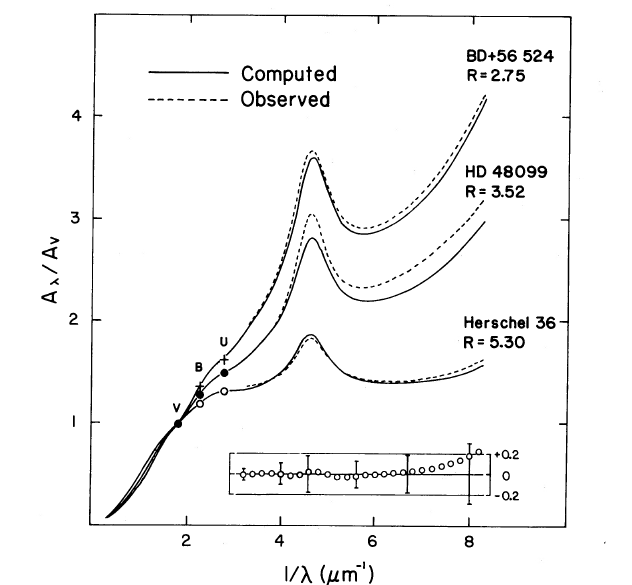
\includegraphics[width=1.0\textwidth]{cardelli_curve_fig4_crop.png}
\caption{Variation of the extinction, normalised to the $V$-band extinction $A_{V}$, as a function of wavelength, in spectral regions ranging from the IR (left) to the UV (right). The solid lines are calculated using Equation \ref{CCM_general} at the given $R_{V}$ values. These values represent the lines of sight for their respective source stars, which are listed alongside.  Source: \cite{1989ApJ...345..245C}}
\label{cardelli_curve}
\end{center}
\end{figure}

\cite{1985ApJ...288..618R} found that outside dense molecular clouds, which have high opacities and whose lines-of-sight are less frequently used as a result, all extinction laws for all studied Johnson-Cousins filters \citep{1953ApJ...117..313J}, which have long been the standard set of filters in UV-IR spectral observations, were uniform between wavelengths of 1 and 13 $\mu$m when observing sources in the direction of the Galactic Centre. This result was then used to produce constant ratios of the extinction in those filters ($A_{X}$, where $X$ represents a generic photometric filter) to the extinction in the Johnson-$V$ filter ($A_{V}$). This ratio is denoted by $A_{X}/A_{V}$. They also determined the now-widely used global average value of 3.08 ($\sim$3.1) for $R_{V} \equiv A_{V}/E(B-V)$, known as the total-to-selective extinction ratio,  for the diffuse ISM. \\*

\cite{1989ApJ...345..245C} used observations of mostly bright, hot O- and B-type main-sequence stars to produce empirical equations describing the mean ratio of extinction values at a specific wavelength $\lambda$ ($A_{\lambda}$) to the $V$-band extinction, this ratio being denoted by $A_{\lambda}/A_{V}$. The study produced a basic equation of the form:

\begin{equation}
A_{\lambda}/A_{V} = a(x) + b(x)/R_{V},
\label{CCM_general}
\end{equation}

where $x \equiv 1/\lambda$. The significance of $R_{V}$, as noted in the same paper, comes from its usefulness as an indicator of the nature of the interstellar medium through which the observed light travels in order to reach the observer. The total wavelength range was divided into 4 sub-ranges, each with a governing pair of empirically-determined equations to calculate $a(x)$ and $b(x)$, respectively. The resulting extinction-ratio profiles for three lines of sight are displayed in Figure \ref{cardelli_curve}. This model underpins more recent studies of intrinsic effects on extinction \citep{2008PASP..120..583G,2014MNRAS.444..392C,2018MNRAS.475.5023C,2018MNRAS.479L.102C}, and provides the basis for the synthetic $A_{X}/A_{V}$ datasets in this project. Equation \ref{CCM_general} has become a standard model for theoretical studies to employ for predictions made in the UV, optical and near-IR wavelength regions, although it is not always accurate \citep{1994ApJ...422..158O,1999PASP..111...63F}. \\*

\cite{1994ApJ...422..158O} found deviations from the \cite{1989ApJ...345..245C} extinction law in the soft-UV spectral range using a sub-sample of 22 stars from the same dataset. This was attributed to the uncertainty in the short-wavelength cutoff of the UV-range Johnson $U$ filter and to the presence of the Balmer discontinuity within the limits of the filter bandpass.\\*

\cite{1999PASP..111...63F} found that, due to the broadband nature of the Johnson filters and the general decrease of extinction with wavelength, the \cite{1989ApJ...345..245C} relations overestimate the extinction in the near-IR and blue-visible Johnson filters. The study put forward corrections to the equations for $a(x)$ and $b(x)$ for these wavelength regions. However, in the UV region covered by  the \cite{1989ApJ...345..245C} equations, the equations are accurate for 93\% of a homogeneous UV observational database \citep{2004ApJ...616..912V}.\\*

\cite{2014MNRAS.444..392C,2018MNRAS.475.5023C,2018MNRAS.479L.102C} created simple  models for the parameter $R_{X}  = \frac{A_{X}}{E(B-V)}$, consisting of a quadratic variation with effective temperature and a linear variation with metallicity (they found no significant variations with surface gravity) in multiple telescope filter systems. This was based on MARCS model stellar atmospheres, which have an upper effective temperature limit of 8000K \citep{2008A&A...486..951G}. The equation is independent of surface gravity and has the following form:

\begin{equation}
R_{X} = a_{0} + T_{4}(a_{1} + a_{2}T_{4}) + a_{3}\textnormal{[Fe/H]}
\label{casagrande_ext_fit}
\end{equation}

where $T_{4} = 10^{-4} \times T_{\textnormal{eff}}$ and $T_{\textnormal{eff}}$ is the effective temperature. The equation is valid for $5250\textnormal{K} \leq T_{\textnormal{eff}} \leq 7000\textnormal{K}$. Although these models are mathematically simple (with only 4 coefficients), the limited $T_{\textnormal{eff}}$ range in which they are applicable is problematic, particularly in the red giant branch (RGB) and lower main sequence of any stellar population.\\*

\section{Extinction in stars \& stellar populations}

\subsection{The effect of extinction on the observed magnitudes of different stellar types} \label{params}

%To understand the effect of different stellar types with respect to the calculated interstellar extinction

This project examines the effect of extinction treatment methods on interpretations of observed stellar populations. To understand how extinction affects the observed magnitudes of different stellar types, we must first define the fundamental parameters that describe a stellar atmosphere, which will be used in this project as the input variables on which any star-to-star variations in extinction will be modelled. \\*

\begin{figure}[h!]
\begin{center}
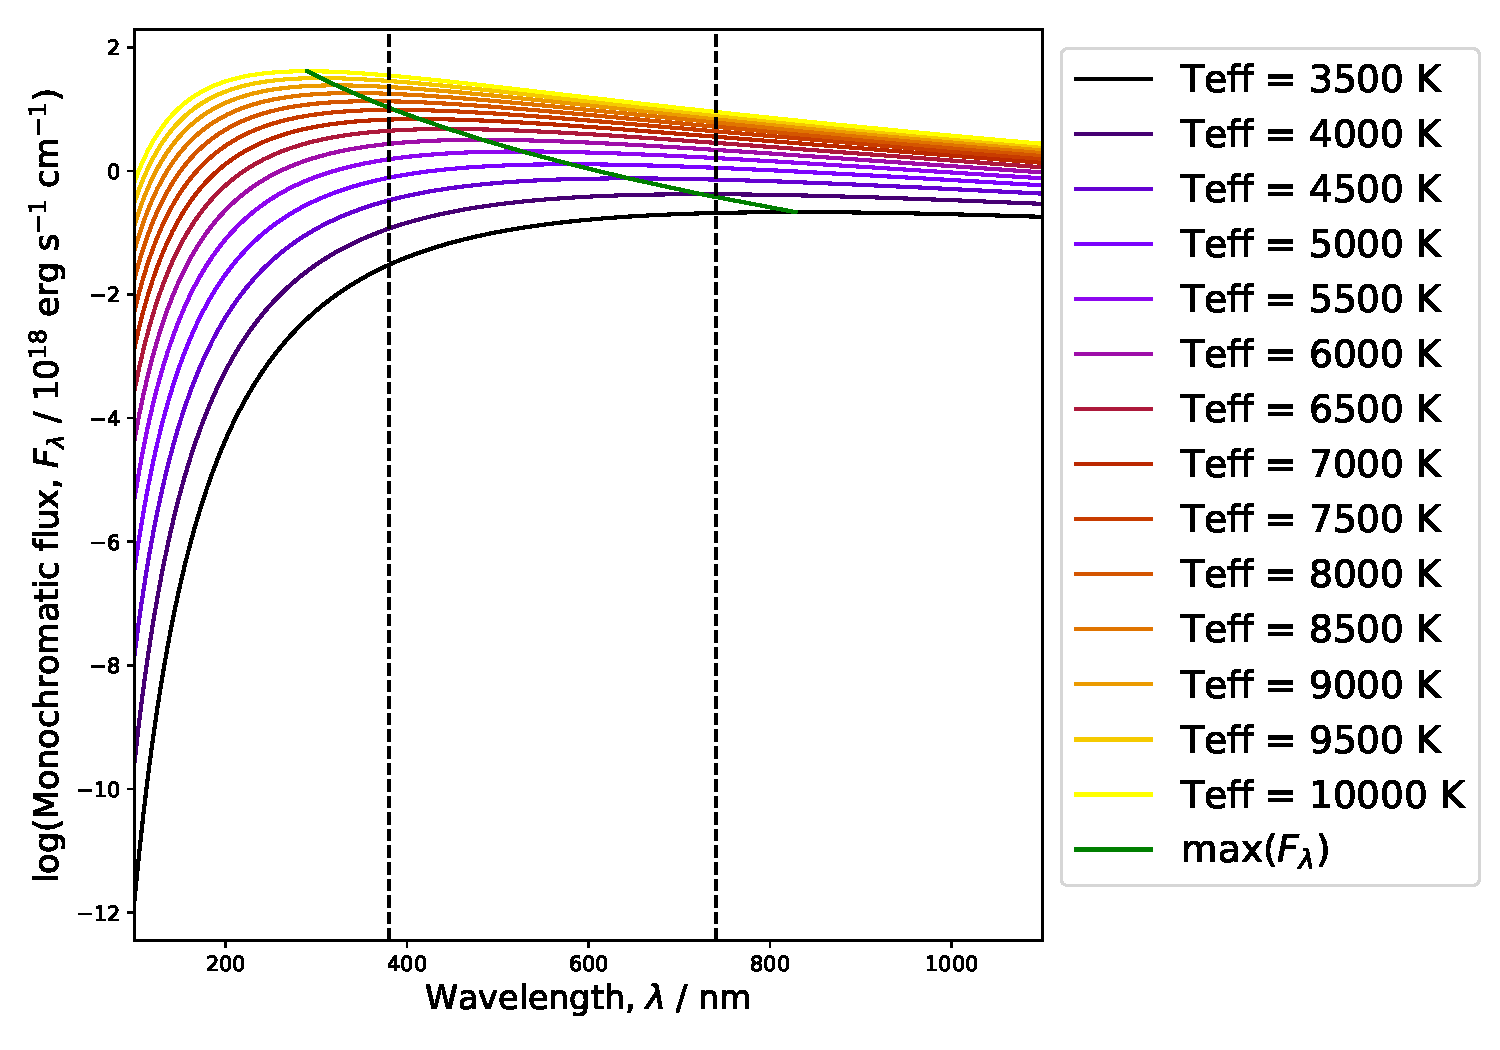
\includegraphics[width=1.0\textwidth]{blackbody_teff_logF_illustration.pdf}
\caption{Plot of the logarithm of monochromatic flux of a black body for different stellar effective temperatures, as a function of wavelength. The black dashed lines mark the approximate limits of the visible part of the EM spectrum. The green curve represents the variation of the Planck Law maxima with effective temperature.}
\label{planck_curve}
\end{center}
\end{figure}

The effective temperature ($T_{\textnormal{eff}}$) of a star is defined as the thermodynamic temperature of a black body which produces the same stellar flux across all wavelengths (known as the bolometric flux) as that produced by the star. The equation of the radiation emitted by a black body produces the body's flux per unit wavelength per unit angular viewing area, $F_{\lambda,bb}$, known as the black body's monochromatic flux. The equation, known as the Planck Law, is as follows:


\begin{equation}
F_{\lambda,bb} = \frac{2hc^{2}}{\lambda^{5}\left(\exp\left({\frac{hc}{\lambda k_{B}T}}\right) - 1\right)}
\label{planck_bb}
\end{equation} 

where $T$ is the thermodynamic temperature of the black body, $h$ is Planck's constant, $c$ is the vacuum speed of light and $k_{B}$ is Boltzmann's constant. This equation also holds if the light wave frequency is used instead of the wavelength, with the monochromatic flux $F_{\nu,bb}$ now being the black body flux per unit frequency per unit angular viewing area:

\begin{equation}
F_{\nu,bb} = \frac{2h\nu^{3}}{c^{2}\left(\exp\left({\frac{h\nu}{k_{B}T}}\right) - 1\right)}
\label{planck_bb_freq}
\end{equation}

In this project, the definition of monochromatic flux for any given object will be reserved exclusively for the flux per unit wavelength, $F_{\lambda}$, with any calculations involving black body fluxes using Equation \ref{planck_bb}. \\*

The general approximation of stars to black bodies (and hence the actual stellar surface temperature to $T_{\textnormal{eff}}$) is valid because all stars have been observed to have spectra that closely resemble those of black bodies, with the notable exception of atmospheric absorption lines. The (intrinsic) bolometric luminosity of a star is used to define the effective temperature via:

\begin{equation}
L = 4 \pi R^{2} \sigma_{SB} T_{\textnormal{eff}}^{4}
\label{Teff_def}
\end{equation}

where $R$ is the (mean) stellar radius. Effective temperature has an effect on interstellar extinction due to its strong effect on the stellar luminosity and, hence, the flux, via the Planck Law in Equation \ref{planck_bb}. For a higher effective temperature, as demonstrated in Figure \ref{planck_curve}, there will be more photons in the broad beam of light with wavelengths that make them likely to interact with the local ISM. \\*

Different chemical elements have different orbital configurations of atomic/ionic electron states. Each electron state absorbs and emits photons at a particular wavelength, which varies between individual states and between elements. Therefore, a greater proportion of light in a broadband beam is absorbed in a medium containing a mixture of many different elements than in a medium dominated by one or two elements. From astrophysical observations, it is clear that hydrogen is by far the most abundant element in the universe, with helium a clear-but-distant second. The metallicity of a star is defined as the fractional abundance of heavy elements, often approximated by iron (Fe) alone, relative to the star's hydrogen (H) abundance, compared to that of the Sun. The abundances are determined by the strength of the elements' characteristic atomic absorption lines in the stellar spectra.

\begin{equation}
\textnormal{[Fe/H]} = \log\left(\frac{N_{\textnormal{Fe}}}{N_{\textnormal{H}}}\right) - \log\left(\frac{N_{\textnormal{Fe},\odot}}{N_{\textnormal{H},\odot}}\right)
\label{FeH_def}
\end{equation}

For a generic atomic species $E$, $N_{E}$ represents its number density. For stellar observations, $N_{E}$ is measured at the surface. Since the output of Equation \ref{FeH_def} is logarithmic, a value of [Fe/H] = 0 indicates solar metallicity. An increase in metallicity would cause the corresponding absorption lines to be stronger, thus reducing the observable flux. An increased metallicity also implies an increase in abundance of sub-ferrous metals. The presence of more nuclear species, each with unique absorption line configurations, inevitably creates more observable lines, further increasing the apparent extinction in the spectral flux. The effect of this reduction in flux manifests itself as a reduction in the stellar luminosity and therefore the effective temperature when all other stellar properties (such as the mass and age) are fixed.\\*

The definition of the stellar surface gravity $g$ is simply the value of the standard Newtonian gravitational acceleration, applied to the stellar surface (the mass is the total stellar mass, $M$, and the distance is the stellar radius, $R$):

\begin{equation}
g = \frac{GM}{R^{2}} = \frac{4\pi G\int_{0}^{R}\rho(r)r^{2}dr}{R^{2}}
\label{gravity_def}
\end{equation}

A greater surface gravity, as can be inferred from Equation \ref{gravity_def}, represents a surface with a higher mass density. For stars, being self-gravitating, this infers a higher atomic number density.  \\*

%the effect of atomic number density on

The effects of surface gravity on the stellar emission spectrum arise directly from the quantum properties of the interactions between the photons and atomic electrons in the stellar atmosphere. When a particle, such as an electron, absorbs a photon, the absorption process is not instantaneous and therefore carries an uncertainty in the time taken for the process to be completed, with a corresponding uncertainty in energy due to the Heisenberg uncertainty principle. Across a large number of absorptions for the same initial electron state, the result is a spread in the energies of the absorbed photons. The associated emission line is therefore broadened by the multiple wavelengths of the photons. This is universal and referred to as ``natural broadening''.\\*

The impact of surface gravity arises via additional broadening effects upon these same absorption lines due to more inter-atomic interactions caused by a greater atmospheric atomic number density, which impact that states of atomic electrons. When broadening effects are applied to an emission spectrum, such as a spectrum from a stellar surface, the result is that fewer photons pass through the surface, thereby reducing the surface flux seen by an outside observer. \\*

The impact of stellar effective temperature, metallicity and surface gravity on extinction arises through their described effect on the spectral energy distribution (SED) emitted by the stellar atmosphere. Since both the SED and the magnitude of the interstellar extinction are functions of wave3.4length, different stellar types, with different SEDs, can be impacted to different extents by interstellar extinction at a given wavelength.

\subsection{Forbes effect} \label{forbes}
The Forbes effect occurs as a broadband beam of light, such as that emitted by a star, passes through an extended partially-transparent medium, such as the Earth's atmosphere or an interstellar gas or dust cloud. It states that the greater the distance travelled by a light beam through the medium, the more penetrating the beam becomes \citep{1842RSPT..132..225F}. The physical basis for this effect is that those photons in the original beam whose wavelengths make them the most likely to be absorbed or refracted are, on average, the earliest to be separated from the beam path as the beam through the medium. Therefore, as the beam travels through the medium, its constituent photons are progressively less likely to be interact with the medium \citep{1995A&AS..109..293G}. Since a higher fraction of its photons are retained as the distance through the medium increases, the beam is more penetrating \citep{OHVRIL1999305}.\\*

This has the effect of producing a non-linear increase in extinction for one filter relative to the increase in another \citep{1995A&AS..109..293G,2008PASP..120..583G}. It should be emphasised that the Forbes effect occurs regardless of the source star's spectral type, and therefore represents an additional source of uncertainty when calculating extinction for highly-reddened stellar populations. \\*

\subsection{Determining properties of stellar populations}
\subsubsection{The role of CMDs} \label{CMDs_intro}
If we compare the individual black body spectra in Figure \ref{planck_curve}, it can be seen that the maximum monochromatic flux of the black body occurs at an increasingly shorter wavelength for objects with increasingly higher temperatures, as indicated by the green curve connecting the $F_{\lambda,bb}$ maxima at different temperatures. This makes the object appear bluer to an observer. The relationship between the wavelength at which the monochromatic flux is maximal ($\lambda_{max}$) and the black body temperature is quantified by Wien's displacement law:

\begin{equation}
\lambda_{max} T = 2.898 \times 10^{6} \textnormal{ nm K}
\label{wien_eq}
\end{equation}

More importantly, Figure \ref{planck_curve} demonstrates that, within the UV-to-IR wavelength regime, the change in monochromatic flux between values at two different wavelengths is always greater for stars with higher effective temperatures. Therefore, to measure a star's effective temperature, observers compare the star's observed flux in two filters operating at different wavelengths within this range. The difference between the star's flux magnitudes in each of the two filters is then taken, with the flux in the redder filter being deducted from that of the bluer filter. This quantity is known as the colour index. For two filters $X$ and $Y$, with $X$ being bluer than $Y$, the colour index of observations made using those filters, $(X-Y)$, is defined as:

\begin{align}
\begin{split}
(X-Y) &= m_{X} - m_{Y} \\
 &= (m_{X,0} - m_{Y,0}) + (A_{X} - A_{Y}) \\
 &= (X-Y)_{0} + E(X-Y)
\end{split}
\label{colour_index}
\end{align}

where $(X-Y)_{0}$ is the true or intrinsic colour index of the object, $m_{X,0}$ and $m_{Y,0}$ are the object's intrinsic apparent magnitudes in $X$ and $Y$, respectively, and $E(X-Y) = A_{X} - A_{Y}$ is known as the colour excess, but can also be denoted in literature using the term ``reddening''. The colour excess represents the effect of extinction on the observed colour index. Its importance arises from the prominence of the intrinsic colour index in determining effective temperature. Higher values of $(X-Y)$ indicate redder stars, with lower effective temperatures.\\*

The most commonly-used colour index, employed as a reference for most optical observations, is the Johnson ($B-V$) index \citep{1953ApJ...117..313J}. This is due to these filters being the among most widely-used and best-studied available, allowing for better comparisons of different data, including data from older archives.\\*

It can be seen from Equation \ref{Teff_def} that the luminosity (and therefore flux) of a star is dependent on radius as well as effective temperature. If a plot is made of luminosity against effective temperature (a Hertzsprung-Russell diagram), it can be seen that all stars in a given star cluster follow a single, complex track. Because the stars are approximately the same age in a typical cluster population, this track is know as an isochrone. Isochrones for different population ages and metallicities are calculated using theoretical stellar models, which cover the largest possible spread of initial stellar masses for the required age.\\*

By examining the flux-magnitude equations from both this section and Section \ref{ext_def}, it becomes clear that both the absolute filter magnitudes and the intrinsic colour indices can be used, together with bolometric corrections, to calculate the luminosity from observational data. To determine the detailed properties of stellar populations, all stars in an observational sample or star cluster are plotted together on a pair of axes known as a colour-magnitude diagram (CMD), which represents an observational analogue of the HR diagram \citep{2005ARA&A..43..293B}. The absolute magnitude of stars in a given filter $Z$, $M_{Z}$, is on the vertical axis, with the flux increasing (and the magnitude value decreasing) upwards. The intrinsic colour index of the stars in two filters $X$ and $Y$, $(X-Y)_{0}$, is on the x-axis, with the values increasing (and stars becoming redder) to the right. Note that filter $Z$ may be the same as either $X$ or $Y$.\\*

In practice, the universal general shape and position of stellar populations in the HR diagram and each observational CMD, particularly the position and shape of the main sequence, provides a highly useful tool for comparing stellar populations with unknown distances and extinction values to known examples and to theoretical models. This is done by alignment of the respective main sequences in CMDs, particularly the upper main sequence below the MSTO position, which contains the most luminous MS stars and is less sensitive to the (initially unknown) value of the cluster metallicity than the lower MS. \\*

The age of an observed stellar population is determined by, firstly, correcting the data for the effects of distance and extinction and, secondly, aligning a series of isochrones, each of a different age, with the main-sequence (MS) of the observed data. The accepted age of the population is that of the isochrone which most closely follows the progression of stars along the main-sequence turn-off (MSTO). As such, any errors in the estimated extinction can potentially change the age of the best-fit isochrone and therefore produce an erroneous estimate of the true population age.

\subsubsection{Comparing theoretical and observational quantities} \label{add_ext}
For any observational dataset of stars, the stars' individual extinction values will be completely unknown from the data alone. In order to compare observational and theoretical data, the most convenient approach is to add the (theoretical) extinction value(s) to the theoretical dataset magnitudes (i.e., absolute magnitudes), before comparing to the distance-corrected observational data. As a result, the quantity from each dataset that is being compared is the absolute magnitude plus the extinction in each filter. If we label this quantity $M_{\textnormal{ext},X}$ for a generic filter $X$, we can define it as:

\begin{equation}
M_{\textnormal{ext},X} = M_{X} + A_{X}
\label{MextX_def}
\end{equation}

Using Equation \ref{ext_def_app_mag}, Equation \ref{MextX_def} can now be rewritten such that $M_{\textnormal{ext},X}$ can be defined using both quantities derived directly from observations and those determined by theoretical models:

\begin{align}
\begin{split}
M_{\textnormal{ext},X} &= M_{X} + A_{X} \textnormal{ (theoretical data)}\\
 &= m_{X} + 5 - 5\log\left(\frac{d}{\textnormal{pc}}\right) \textnormal{ (observational data)}
\end{split}
\label{MextX_eq}
\end{align}

This allows for direct comparison of theoretical data, whose stars are treated with theoretically-determined $A_{X}$ values, with distance-corrected observational data, whose stars have unknown $A_{X}$ values. Equation \ref{MextX_eq} therefore provides a pathway for comparing the standard treatment of extinction (constant $A_{X}/A_{V}$ ratios) with the treatment proposed in this project ($A_{X}/A_{V}$ varying as functions of intrinsic stellar parameters). In practice, therefore, due to the unknown extinction values for the individual stars and the cluster as a whole, the axis parameters for the generic CMD in Section \ref{CMDs_intro} are $M_{\textnormal{ext},Z}$ and $(X-Y)$, instead of $M_{Z}$ and $(X-Y)_{0}$, respectively.\\*

\section{The standard treatment of extinction in observed stellar populations} \label{standard_ext}

In observations, the extinction for a given source is initially unknown. For a stellar population, observers must make use distinctive features of stellar populations that can be used as standard candles to estimate the distance to the population. \\*

The treatment of extinction in observational surveys is usually via a constant value for the ratio of extinction in a given filter $X$, denoted by $A_{X}$, divided by the extinction in the well-studied Johnson-$V$ filter, $A_{V}$. The value used for this ratio, denoted by $A_{X}/A_{V}$, is often taken from \cite{1985ApJ...288..618R}. This approach has the significant issue of producing $A_{X}/A_{V}$ values that do not account for  variations between stellar spectra due to different physical parameter values in different stellar atmospheres when integrated over the filter's wavelength range. As shown in Figure \ref{planck_curve}, the monochromatic flux at a given wavelength varies greatly with effective temperature, as does the ratio between monochromatic fluxes of stars of different temperatures. This makes the notion that stars of different temperatures lose the same flux in a given filter, which is implied by the use of constant extinction ratios across all stellar types, inherently flawed. As shown in Figure \ref{planck_curve}, stars with higher effective temperatures have emission spectra with both significantly higher fluxes at all wavelengths and proportionally greater fluxes at the shorter wavelengths in the UV-IR spectral range which are most impacted by interstellar extinction. Therefore, it should be expected that hotter stars experience higher extinctions $A_{X}$ for a given filter, not equal values.\\*

\cite{2008PASP..120..583G} produced data tables of $A_{X}/A_{V}$ for stellar atmosphere models with parameters $T_{\textnormal{eff}}$, log($g$) and [Fe/H]. They carried this out using the same ATLAS9 data \citep{2004astro.ph..5087C} that was used to generate the data for this project, but also combined it with data from other studies, which are listed in \cite{2002A&A...391..195G}, resulting in data covering a parameter space extending beyond the ATLAS9 limits in all three parameters. They used the data tables to calculate the $A_{X}/A_{V}$ values for the stellar models in Padova theoretical isochrones. While determining that the values of $A_{X}/A_{V}$ varied significantly with $T_{\textnormal{eff}}$ and log($g$), the variation with metallicity was found to be $\sim$0.17$\%$ between [Fe/H] = 0.0 and [Fe/H] = -2.5. They found that, when they set $A_{V} = 6$, there was a systematic shift for the ACS system between extinction values calculated star-wise using the tables of $A_{X}/A_{V}$ data and a constant extinction value applied to the entire isochrone. The constant values of $A_{X}/A_{V}$ were calculated from a yellow dwarf in the low-extinction regime. Overall, in the single ACS CMD example shown in the study, the $A_{X}/A_{V}$ tables produced a smaller extinction value in the F814W filter and a larger (F475W-F814W) colour index value. It also caused a change in the shape of the curve at the main-sequence turn-off (MSTO) point. They then applied the data from the tables to the case of the globular cluster M92. They found the optimal metallicity to be $Z = 0.0004$ ([Fe/H] $\approx$ -1.6) instead of the value obtain by previous observers of $Z = 0.0001$ ([Fe/H] $\approx$ -2.2). Therefore, their use of $A_{X}/A_{V}$ data caused the estimated cluster metallicity to be greater than when using the standard one-size-fits-all approach to extinction.\\*

\cite{2017Galax...5...28O} used the tabulated extinction ratio tables resulting from \cite{2008PASP..120..583G}, which demonstrated the significant effect of stellar parameters on the calculated extinction ratios, to search for potential discrepancies in the predicted ages of isochrones after the addition of extinction. This was performed for isochrones with real ages between 12 and 13 Gyr and employed a small selection of Johnson ($B$,$V$ and $I$) and ACS (F606W, F775W and F814W) broadband filters. They found that, once the assumption of uniform extinction across the entire population was removed by employing the \cite{2008PASP..120..583G} data, the isochrone position in the CMD shifted such that, at $A_{V} = 1$, the position of the MSTO of a 12 Gyr isochrone with individual stellar extinction values added is the same as the MSTO position for a 12.5 Gyr isochrone with the standard single extinction value added.\\*

\section{Project objective}
The first goal of this project is to investigate the variations of the extinction ratios $A_{X}/A_{V}$ in selected photometric filters within multiple filter systems with changes in effective temperature, surface gravity and metallicity. This will be carried out using a large library of theoretical stellar spectra covering all main stages of stellar evolution. Analytic fitting functions will be employed to model the $A_{X}/A_{V}$ variations in each filter as a function of the stellar parameters. \\*

%This goal of this project is to first investigate how the extinction ratios Ax/Av in selected photometric filters depend on the stellar effective temperature, surface gravity and metallicity, employing a large library of theoretical stellar spectra, that cover all the main stellar evolutionary phases. Analytical fitting functions will be used to model Ax/Av as a function of the stellar parameters.

%As an application of this result, the CMD of a representative open cluster affected by relatively high extinction will be fit with theoretical isochrones. In one case a constant value of the Ax/Av ratios will be applied to the whole isochrone, whilst in a second case varying Ax/Av ratios will be considered. A comparison of the ages and distances derived in the two cases will give a quantitative idea of the importance of considering in CMD fitting Ax/Av ratios that depend on the stellar parameters, instead of the common practice of using constant Ax/Av values.

%Furthermore, this project will attempt to use mathematical functions as models to describe these variations in $A_{X}/A_{V}$. 

%is to use this simplification of the variations to determine the differences in the estimated optimal ages, elemental abundances (i.e., metallicity) and extinction reference values of stellar populations between simulating extinction using values calculated for each star and using a single value for extinction across the entire population, which is the current standard method. If such differences exist and if they are of significant size, it could cause a recalculation of the properties of observed star clusters. This could potentially cause a reinterpretation of these clusters' history, including where and when they formed in the Milky Way and the chemical enrichment of the gas that formed their stars. \\*

The results of the fitting process will then be applied to the CMD of a representative observational example of a relatively high-extinction open cluster. The CMD will be fitted with two theoretical isochrones. For the first case, a constant $A_{X}/A_{V}$ value will be applied to the entire isochrone. For the second, varying $A_{X}/A_{V}$ values will be applied, using the fitting results. The best estimates for the ages and $A_{V}$ values in both cases will be compared, giving a quantitative illustration of the importance of the effect of the stellar parameters on $A_{X}/A_{V}$ ratios used in CMD fitting.\\*



\chapter{Methodology}

\section{Calculating extinction ratio data}

When observing stars through a photometric filter, only a small fraction of the bolometric stellar flux that reaches the telescope is detected, since stars emit photons with wavelengths across the full EM spectrum. This is due to the design of the filter in question, which determines the fraction of photons detected at a given wavelength, known as the transmittance. The variation in transmittance as a function of photon wavelength is known as a transmission curve, bandpass or filter response function. Examples of filter response functions for the photometric systems are given in Figures \ref{Gaia_response_funcs}-\ref{WFC3_response_funcs2}. It is clear that the range of wavelengths for which the transmittance is non-zero, for any filter, is very narrow when compared to the full EM spectral range.\\* 

The significance of this relatively narrow wavelength range occurs when analysing observational data using the results of theoretical stellar models, which determine the state of a stellar evolution model at a specified age. The results of theoretical evolutionary models are expressed in terms of a star's bolometric quantities, such as the bolometric luminosity, the effective temperature and the metallicity, which in turn can be used to calculate further important quantities, such as the stellar radius (via Equation \ref{Teff_def}) and surface gravity (via Equation \ref{gravity_def}). The significance is due to the fact that these evolutionary models are the same models that are used to generate isochrones for stellar populations. In this project, isochrones are the central tool to compare the effects of using variable and fixed extinction ratios on the estimated age of star clusters. Therefore, to correctly compare theoretical models and isochrones, which use bolometric data, to observational photometric data, by necessity limited by the use of filters, mathematical methods must be used to transform the theoretical stellar evolution model data into the form of filter-based fluxes and magnitudes.\\*

\subsection{The role of stellar evolutionary and atmosphere models}
The first step in this transformation is to compute theoretical stellar spectra. This is done using stellar atmosphere models, which use values of $T_{\textnormal{eff}}$, log($g$) and [Fe/H], taken from the appropriate stellar evolution models, as a basis to produce a theoretical emission spectrum for that star, in the form of a table showing a list of desired wavelengths $\lambda$ and the theoretical monochromatic flux at that wavelength, $F_{\lambda}$, defined at the atmospheric/stellar radius, $R$. To apply the spectrum to the case of a distant observer, the equation linking the relevant flux definitions to the observer distance, $d$, must be included:

\begin{equation}
f_{\lambda}d^{2}=F_{\lambda}R^{2}
\label{flux_dist_rd}
\end{equation}


where $f_{\lambda}$ represents the (theoretical) monochromatic flux at a given wavelength $\lambda$ at the observer's distance from the source. However, as with all flux magnitudes, the predicted apparent magnitude for a distant star, with unknown extinction,  must be linked to a known reference point. This requires the detailed knowledge of a reference stellar spectrum, of a star which is least susceptible to significant extinction, meaning, in effect, a nearby object. For all filter systems studied in this project, the nearby bright star Vega ($\alpha$ Lyr) was used as the reference object. Using Vega as the reference star is the most well-known approach to photometric calibration \citep{2014MNRAS.444..392C}.\\*

After accounting for the effect of interstellar extinction on an object's emission, its apparent magnitude in the wavelength range of a generic filter $X$, defined as increasing from the shortest ($\lambda_{1}$) to the longest ($\lambda_{2}$) wavelength for which its response function is non-zero, can be calculated in terms of parameters determine theoretically by both stellar evolution and atmosphere models:

\begin{equation}
m_{X} = -2.5 \log_{10} \left(\frac{ \int_{\lambda_{1}}^{\lambda_{2}} f_{\lambda} \left( 10^{-0.4 A_{\lambda}} \right) S_{\lambda} d\lambda }{ \int_{\lambda_{1}}^{\lambda_{2}} f_{\lambda}^{0} S_{\lambda} d\lambda }\right) + m_{X}^{0}
\label{app_mag_def}
\end{equation}

where $A_{\lambda}$ is the extinction as a function of wavelength (see Equation \ref{ratio_eq} later for calculation of values from the \cite{1989ApJ...345..245C} extinction law), $S_{\lambda}$ represents the filter response function of $X$ and $f_{\lambda}^{0}$ and $m_{X}^{0}$ represent the monochromatic flux and apparent magnitude, respectively, in $X$ of Vega. The use of these two well-determined observational parameters allows the remaining terms to be fixed to a known scale.\\*

%Stars, as mentioned earlier, . Figure \ref{planck_curve} shows that the difference between absolute monochromatic stellar flux for different effective temperatures itself varies significantly as a function of wavelength.
\subsection{Bolometric corrections}

For an observed star at an unknown distance $d$, Equation \ref{flux_dist_rd} cannot give the magnitude of the theoretical spectrum at the observer distance, $f_{\lambda}$ with any reasonable certainty. This then causes uncertainty regarding the extinction $A_{\lambda}$ given its position in the same integrand in Equation \ref{app_mag_def}. The equation does, however, have great value via the inclusion of the well-constrained observed Vega quantities. Therefore, the uncertainty arising from $f_{\lambda}$ must be eliminated. This is best achieved by considering the problem in terms of the absolute magnitude, $M_{X}$, of the star in filter $X$, rather than the apparent magnitude. This first requires the use of the standard equation linking the two:

\begin{equation}
M_{X} = m_{X} - 2.5 \log_{10}\left( \left( \frac{d}{10 \textnormal{pc}} \right)^{2} \right),
\label{abs_mag_def}
\end{equation}

This represents the second step required for the comparison of theoretical isochrones to the observational case, and requires the calculation of bolometric corrections. To derive the equation linking a bolometric correction with the extinction parameter, we start with the definition of a bolometric correction for filter $X$, which is denoted by $BC_{X}$:

\begin{equation}
BC_{X} \equiv M_{\textnormal{bol}} - M_{X}
\label{BC_def}
\end{equation}


where $M_{\textnormal{bol}}$ is its (predicted) absolute bolometric magnitude, defined relative to the Sun using:

\begin{equation}
M_{\textnormal{bol}} = M_{\textnormal{bol},\odot} - 2.5 \log_{10} \left( \frac{4\pi R^{2}F_{\textnormal{bol}}}{L_{\odot}} \right)
\label{mbol_sun}
\end{equation}

where $M_{\textnormal{bol},\odot}$ is the solar absolute bolometric magnitude, which is assumed in this work to have a value of 4.75, $L_{\odot}$ is the solar luminosity, for which a value of $3.844 \times 10^{33}$ erg s$^{-1}$ is used, and $F_{bol}$ is the bolometric flux at the stellar surface. It should be noted that $F_{bol}$ is simply equal to $\sigma_{\textnormal{SB}} T_{\textnormal{eff}}^{4}$, and is therefore determined solely by the choice of stellar atmosphere model. The bolometric correction for filter $X$ can therefore be expressed, via Equations \ref{app_mag_def}-\ref{mbol_sun}, purely in terms of extinction, theoretical stellar quantities independent of distance and observationally well-constrained reference parameters:

\begin{align}
\begin{split}
BC_{X} &= M_{\textnormal{bol},\odot} - m_{X}^{0} - 2.5 \log_{10} \left( \frac{4\pi R^{2}F_{\textnormal{bol}}}{L_{\odot}} \right) \\
&+ 2.5 \log_{10} \left( \frac{\int_{\lambda_{1}}^{\lambda_{2}} F_{\lambda} \left( 10^{-0.4 A_{\lambda}} \right) S_{\lambda} d\lambda}{\int_{\lambda_{1}}^{\lambda_{2}} f_{\lambda}^{0} S_{\lambda} d\lambda} \right)
\label{BC_extinc}
\end{split}
\end{align}

The output value of Equation \ref{BC_extinc} therefore varies with changes in the effective temperature, surface gravity and metallicity of the stellar atmosphere model, via $R$, $F_{\lambda}$ and $F_{bol}$, and the extinction$ A_{\lambda}$.\\*

For a filter $X$, the extinction $A_{X}$, equal to $A_{\lambda}$ for the response function of filter $X$, is usually parametrised relative to the extinction in the well-studied Johnson-$V$ filter, $A_{V}$. To extract $A_{X}$, we use the simple relation:

\begin{equation}
A_{\lambda} = \left( \frac{A_{\lambda}}{A_{V}} \right) A_{V}
\label{ratio_eq}
\end{equation}

together with the \cite{1989ApJ...345..245C} extinction law for $A_{\lambda}/A_{V}$, which is monochromatic and therefore must be placed within the integrand of Equation \ref{BC_extinc}. Given that the \cite{1989ApJ...345..245C} extinction law is normalised to $A_{V}$, the value of $A_{V}$ must be specified prior to the calculation of the bolometric correction. Equation \ref{BC_extinc} was implemented twice, once for each of two distinct $A_{V}$ values (for this project these were $A_{V} = 0$, 1). It should be noted that $BC_{X}(A_{V}=0)$ essentially assumes no extinction in any filter. Therefore, two output values were calculated for Equation \ref{BC_extinc}, one for each $A_{V}$ value. The difference between these two outputs was then taken to extract the extinction ratio $A_{X}/A_{V}$, via the following equation \citep{2008PASP..120..583G}:

\begin{align}
\begin{split}
\left(A_{X}/A_{V}\right)A_{V} &= BC_{X}(0) - BC_{X}(A_{V})
\label{BCs_diff}
\end{split}
\end{align}
%\\ &\approx \left(A_{X}/A_{V}\right)A_{V}

Any dependence of the $A_{X}/A_{V}$ data on the measurements for Vega or the Sun from Equation \ref{BC_extinc} is eliminated during the subtraction, as these terms are unaffected by the $A_{\lambda}$ value. However, effects due to the nature of the atmosphere of the stellar source on the extinction ratio will remain present, in the form of the integrations of $F_{\lambda}S_{\lambda}$ and $F_{\lambda}S_{\lambda} \times \left( 10^{-0.4 A_{\lambda}} \right)$, respectively, in the two bolometric correction terms in Equation \ref{BCs_diff}. \\*

The Forbes effect (see Section \ref{forbes}) has an impact on the non-zero $A_{V}$ value chosen for Equation \ref{BCs_diff} because if $R_{V}$ is held constant at the standard diffuse ISM value of 3.1 \citep{1989ApJ...345..245C}, a larger $A_{V}$ value implies a longer path through the ISM, and thus a stronger Forbes effect. According to \cite{2008PASP..120..583G}, any significant impact from the Forbes effect on the values of $A_{X}/A_{V}$ occurs for a chosen $A_{V} \gtrsim 4$. They found that the effect was particularly strong for stars with $T_{\textnormal{eff}} \lesssim 3000$K and that, unsurprisingly, it became greater as the wavelength range covered by the filter response function increased.\\*

\section{Software used}
\subsection{Isochrones}
The isochrones used in this project were generated using the latest Bag of Stellar Tracks and Isochrones (BaSTI) web interface \citep{2004ApJ...612..168P,2018ApJ...856..125H}. The filter systems whose throughput data were employed by BaSTI to generate the fluxes for the isochrones were ACS, WFC3 and Gaia-DR2. It should be noted that the WFC3 isochrone output for BaSTI does not include flux magnitudes for the F300X filter.\\*

To obtain isochrones from the online database, the desired range of isochrone ages, initial metallicity and photometric filter system must be specified. Therefore, the values of these quantities are shared by all stellar objects in any given isochrone. The output from the BaSTI database for each model stellar object gives the object's initial mass and current mass (i.e. after a time equal to the isochrone age), together with the logarithms of the stellar luminosity in solar units ($\log(L/L_{\odot})$) and of the effective temperature in K ($\log(T_{\textnormal{eff}})$), followed by the predicted absolute magnitudes (with zero extinction) of the object in each filter of the system. \\*

\subsection{Stellar atmosphere models}
To generate the predicted stellar flux, pre-calculated ATLAS9 model stellar atmosphere spectra \citep{1993KurCD..13.....K} were employed. The spectra came in the form of tables incorporated wavelengths,ranging from 9 nm to 160,000 nm, with a resolution of 2 nm or less in the UV, and the predicted monochromatic flux at those wavelengths. Each table, representing one stellar spectrum, is identified by the surface gravity, effective temperature and metallicity of the stellar atmosphere producing that spectrum. Table 1 of \cite{2004astro.ph..5087C} contains precise details of the coverage of the model atmospheres in ($T_{\textnormal{eff}}$, log($g$)) parameter space, while a brief summary  of the limits of the space is listed in Table \ref{atlas9_input}. Four input metallicities were used for ATLAS9, at values of [Fe/H] = -2, -1, 0 and 0.5, covering the metallicities of most observed globular and open clusters. The data for each metallicity value was subject to the same $T_{\textnormal{eff}}$ and log($g$) coverage in ATLAS9.\\*

\begin{table}
\begin{center}
\begin{tabular}{cccc}
\hline
Parameter / unit & Minimum & Maximum & Number of values \\
\hline
$T_{\textnormal{eff}}$ / K & 3500 & 50000 & 76 \\
log( $g$ / cm s$^{-2}$) & 0.0 & 5.0 & 11 \\
$\textnormal{[Fe/H]}$ & -2.0 & 0.5 & 4 \\
\hline
\end{tabular}
\caption{Ranges for the input parameters for ATLAS9 atmospheric models}
\label{atlas9_input}
\end{center}
\end{table}

To make the results of this project apply to the greatest possible range of stellar types, the model atmospheres being employed must ideally be able to reproduce all observed stellar types. Since ATLAS9 atmospheres are constructed from a grid of $T_{\textnormal{eff}}$ and log($g$) values \citep{2004astro.ph..5087C}, the simplest method of ascertaining their applicability is to obtain the widest possible range of $T_{\textnormal{eff}}$ and log($g$) values for the stellar objects which make up the isochrones being employed.\\*

However, the BaSTI data format for a given isochrone does not include explicit values of the surface gravities or radii of the constituent stars. Therefore, to derive the surface gravity $g$ of a given star, we must combine Equation \ref{Teff_def}, to derive the stellar radius, and Equation \ref{gravity_def}, resulting in the following definition of $g$:

\begin{equation}
\label{gravity_LT_calc}
g = \frac{4 \pi G M_{*} \sigma_{\textnormal{SB}} T_{\textnormal{eff}}^{4}}{L_{*}}
\end{equation}

After this had been completed for all points along an isochrone, each star had a co-ordinate in ($T_{\textnormal{eff}}$, log($g$)) parameter space, plus the metallicity of the overall isochrone model. These co-ordinates were then plotted over the grid of co-ordinates for which ATLAS9 spectra were available, as listed in Table 1 of \cite{2004astro.ph..5087C}. The results are shown in Figure \ref{Teff-logg coverage}, using stars in isochrones with ages of 50 Myr (red points) and 12 Gyr (black points). The blue points represent the ATLAS9 model grid, which, in fact, extends to the left beyond the $T_{\textnormal{eff}}$-scale presented in the figure, up to a $T_{\textnormal{eff}}$ value of 50,000 K.\\*

With the exception of the very coolest, and therefore faintest, main sequence stars in the bottom right of the figure, it is clear from Figure \ref{Teff-logg coverage} that the ATLAS9 $T_{\textnormal{eff}}$-log($g$) grid covers the required parameter space for isochrones of all ages including extremely young and extremely old clusters. Any changes in the position of the isochrones in the ($T_{\textnormal{eff}}$, log($g$)) plane at the plotted ages due to a change in metallicity were found to have an insignificant impact on the overlap between the ATLAS9 grid and both isochrones in the ($T_{\textnormal{eff}}$, log($g$)) plane. \\*

This near-complete coverage of stellar objects in isochrones at all ages allows the ATLAS9 data to be applied to the MSTO locations at all isochrone ages, which ensures the applicability of the best-fit isochrone parameter comparisons (see Section \ref{isoc_fit} later) to populations of all ages. Therefore, ATLAS9 is a suitable basis from which start calculating bolometric corrections and therefore, via Equation \ref{BCs_diff}, extinction ratios. \\*

\begin{figure}[h]
\begin{center}
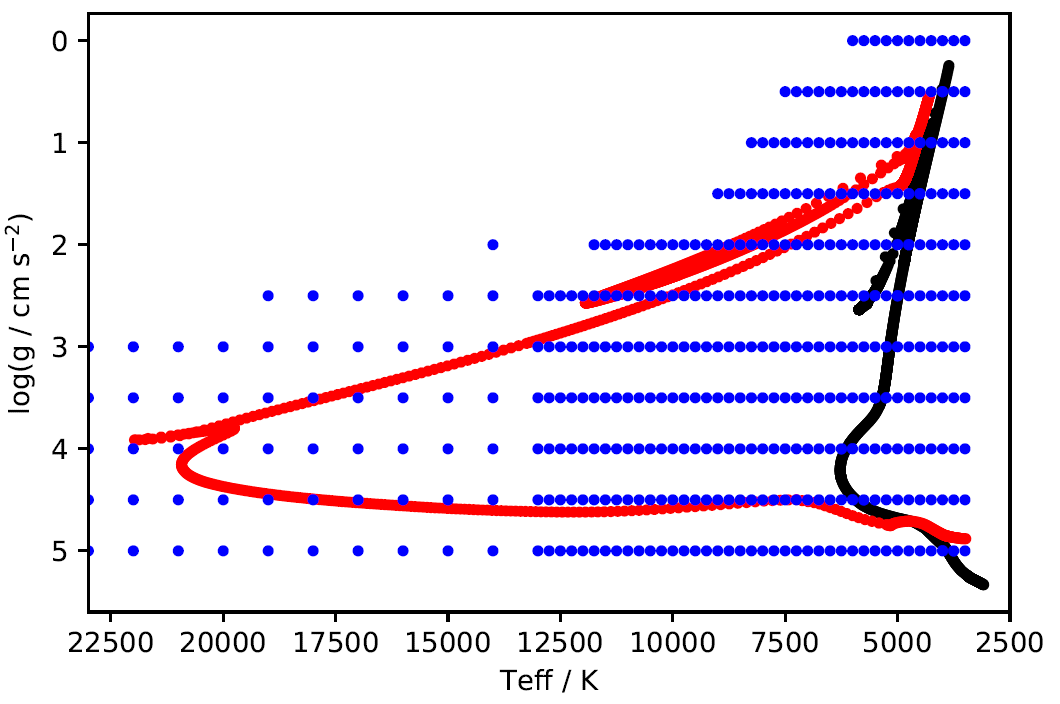
\includegraphics[width=1.0\textwidth]{ATLAS9_grid_BaSTI_coverage_2ages_crop.png}
\caption{$T_{\textnormal{eff}}$-log($g$) scatter plot for a BaSTI 50 Myr, [Fe/H] = -1 isochrone (red), a BaSTI 12 Gyr, [Fe/H] = -1 isochrone (black) and ATLAS9 model grid (blue) for $T_{\textnormal{eff}} \leq 23000$ K.}
\label{Teff-logg coverage}
\end{center}
\end{figure}

\subsection{Programming languages}
The tables of bolometric corrections were generated using a FORTRAN 77 code which incorporated Equations \ref{BC_def}-\ref{BCs_diff} and input data files with tables describing the response functions of all relevant filter systems (described in detail in Section \ref{filter_desc}) at the same wavelengths as those listed in the ATLAS9 model atmosphere tables, with the number of tables for each stellar metallicity value equal to the total number of ($T_{\textnormal{eff}}$, log($g$)) combinations available.\\*

Once the bolometric correction tables were produced, all subsequent processes, including the subtraction required to obtain $A_{X}/A_{V}$ shown in Equation \ref{BCs_diff}, were written in Python 2.7 in the form of an IPython notebook. The repository containing all data, plots and programme codes for this project can be found at \protect\url{https://github.com/AlexlwAstro/phd_work}.\\*

\section{Filters studied} \label{filter_desc}
In this project, three broad-band filter systems were employed. Two are systems on board the Hubble Space Telescope (HST). These are the Advanced Camera for Surveys (ACS), installed in 2002 on the HST \citep{2007AJ....133.1658S}, and the Ultraviolet Imaging Spectrograph channel of the Wide-Field Camera 3 (WFC3/UVIS), installed on the HST in 2009 \citep{2010wfc..rept...14K,2010SPIE.7731E..0ZM}. The third is the single set of three broadband filters mounted on the Gaia space observatory \citep{2010A&A...523A..48J}, launched in 2013. \\*

Examples of response functions for the three filter systems employed in this project are shown in Figures \ref{Gaia_response_funcs}-\ref{WFC3_response_funcs2}. By comparing these with the filters' information in Table \ref{filter_basics}, it can be seen that the exact shape of the response function has a significant impact on the observed flux, as shown in its contribution to the value of the apparent magnitude in Equation \ref{app_mag_def}.\\*

Reference will also be made to the Johnson-Morgan UBV filter system (often simply known as the Johnson system) \citep{1953ApJ...117..313J}, later extended as the Johnson-Cousins UBVRI \citep{1990PASP..102.1181B} system, which has been in use for decades and continues to be be the standard reference for more modern filter systems. Of particular importance are the Johnson blue ($B$) and yellow ($V$) filters, as these formed the original benchmark for observing stellar populations and evolutionary stages. \\*

\begin{figure}[h!]
\begin{center}
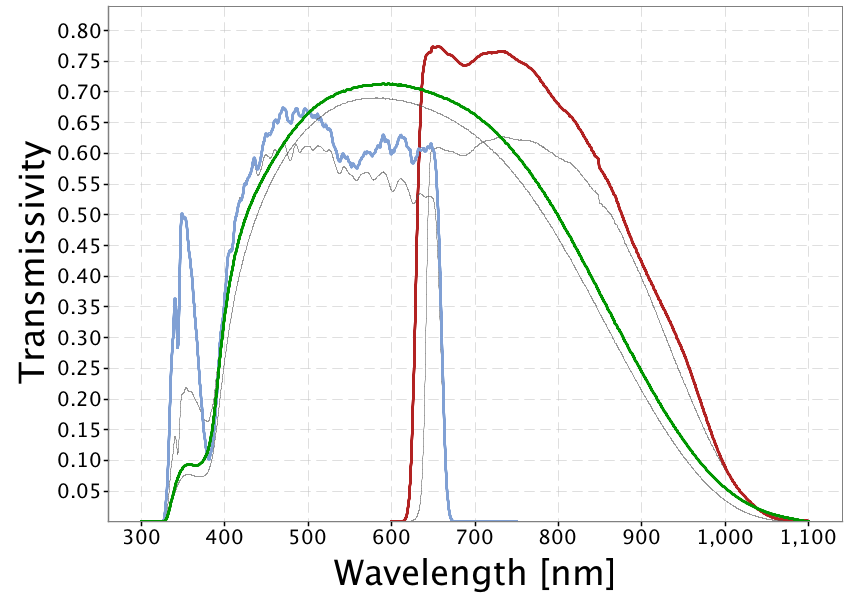
\includegraphics[width=1.0\textwidth]{GaiaDR2Passbands.png}
\caption{Filter response functions for Gaia photometric filters. Source: \protect\url{https://www.cosmos.esa.int/web/gaia/iow_20180316}}
\label{Gaia_response_funcs}
\end{center}
\end{figure}

\begin{figure}[h]
\begin{center}
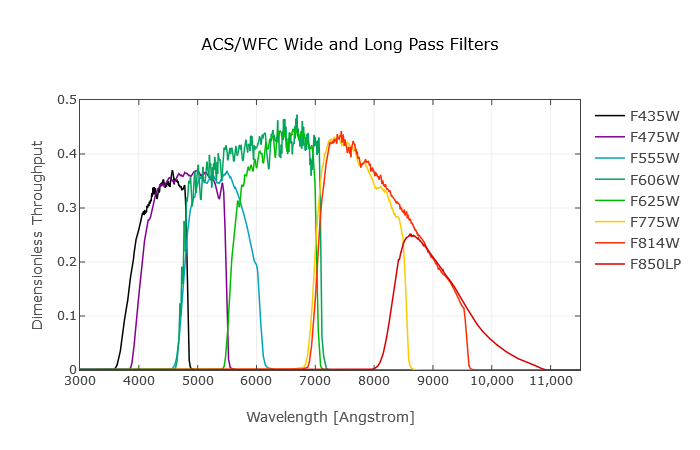
\includegraphics[width=1.0\textwidth]{ACS_Wide.png}
\caption{Filter response functions for wide-field ACS filters. Source: \protect\url{http://www.stsci.edu/hst/acs/analysis/throughputs}}
\label{ACS_response_funcs}
\end{center}
\end{figure}

\begin{figure}[h!]
\begin{center}
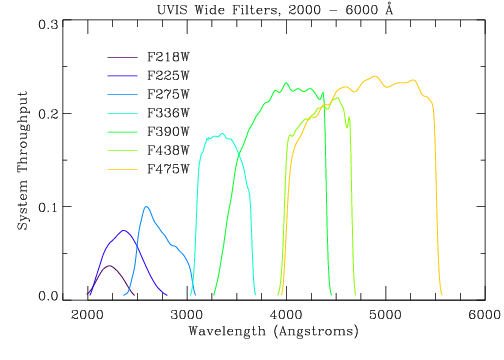
\includegraphics[width=1.0\textwidth]{UVIS_Wide1.jpg}
\caption{Filter response functions for wide-field WFC3 filters. Source: \protect\url{http://www.stsci.edu/hst/wfc3/ins_performance/throughputs/UVIS_filterthru.html}}
\label{WFC3_response_funcs1}
\end{center}
\end{figure}

\begin{figure}[h]
\begin{center}
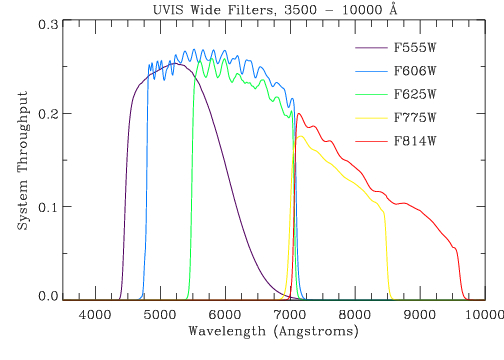
\includegraphics[width=1.0\textwidth]{UVIS_Wide2.jpg}
\caption{Filter response functions for wide-field WFC3 filters. Source: \protect\url{http://www.stsci.edu/hst/wfc3/ins_performance/throughputs/UVIS_filterthru.html}}
\label{WFC3_response_funcs2}
\end{center}
\end{figure}

The standard treatment of extinction for isochrones in CMDs is to apply a single constant value of the extinction ratio for a given filter $X$ to all objects in the isochrone. This quantity is usually expressed as a fixed extinction ratio $A_{X}/A_{V}$ of the (constant) coefficient value in the Johnson-$V$ filter, the standard visual comparison filter. This value is maintained for all stars, regardless of the different effective temperatures, metallicities or surface gravities of the different types of stars present in any given population. The wavelengths of optical light lie between 3800 \AA\ and 7400 \AA, with the $V$ filter having a central wavelength of 5500 \AA.

\begin{table}
\begin{center}
\begin{tabular}{cccccc}
\hline
System & Filter & $\lambda_{\textnormal{cen}}$ / \AA & FWHM / \AA & $\lambda_{\textnormal{min}}$ / \AA & $\lambda_{\textnormal{max}}$ / \AA \\
\hline
% results: previously listed & from source website specified in caption					added more info: l_min & l_max
& F435W & 4359 & 881 & 3610 & 4860 \\ % & 4760 & 729
& F475W & 4781 & 1403 & 3863 & 5563 \\ % & 5000 & 986
& F555W & 5413 & 1236 & 4584 & 6209 \\ % & 5060 & 841
ACS & F606W & 5961 & 2255 & 4634 & 7180 \\ % & 6690 & 1566
& F625W & 6323 & 1390 & 5446 & 7100 \\ % & 6480 & 978
& F775W & 7763 & 1517 & 6804 & 8632 \\ % & 7320 & 1017
& F814W & 8117 & 2096 & 6885 & 9648 \\ % & 7460 & 1657
\hline
& F218W & 2216 & 329 & 1990 & 2603 \\ % & 2175 & 300
& F225W & 2341 & 464 & 1990 & 2968 \\ % & 2250 & 500
& F275W & 2696 & 417 & 2282 & 3119 \\ % & 2750 & 500
& F300X & 2722 & 660 & 2137 & 4098 \\ % &  & 2775
& F336W & 3368 & 550 & 3014 & 3707 \\ % & 3375 & 550
& F390W & 3929 & 951 & 3255 & 4470 \\ % & 3900 & 1000
WFC3 & F438W & 4322 & 674 & 3895 & 4710 \\ % & 4320 & 695
& F475W & 4768 & 1482 & 3942 & 5582 \\ % & 4750 & 1520
& F555W & 5262 & 1578 & 4381 & 7045 \\ % & 5410 & 1605
& F606W & 5941 & 2298 & 4700 & 7204 \\ % & 5956 & 2340
& F625W & 6274 & 1573 & 5414 & 7138 \\ % & 6250 & 1550
& F775W & 7725 & 1454 & 6869 & 8571 \\ % & 7760 & 1470
& F814W & 7814 & 1505 & 6978 & 9684 \\ % & 8353 & 2555
\hline
& $G$ & 6631 & 4397 & 3321 & 10515 \\ % & 6730 & 4400
Gaia & $G_{\textnormal{bp}}$ & 5330 & 2530 & 3283 & 6714 \\ % & 5320 & 2530
& $G_{\textnormal{rp}}$ & 7896 & 2956 & 6296 & 10637 \\ % & 7970 & 2960
\hline

\end{tabular}
\caption{Basic properties of the filters employed in this project. See text for details. Source: \protect\url{http://svo2.cab.inta-csic.es/svo/theory/fps3/index.php}}
\label{filter_basics}
\end{center}
\end{table}

In Table \ref{filter_basics}, all the filters used for this project are listed. The name of each filter is displayed alongside its central wavelength ($\lambda_{\textnormal{cen}}$), full-width at half-maximum (FWHM) and the minimum ($\lambda_{\textnormal{min}}$) and maximum ($\lambda_{\textnormal{max}}$) detection wavelengths. Hence, when combined, these filters cover wavelengths from the soft-ultraviolet (soft-UV) to the near-infrared (NIR), including all visible wavelengths. The FWHM is defined as the difference between the lowest and highest wavelength values at which the transmittance value is half of its maximum value for the filter, typically assuming the response function can be approximated as a Gaussian distribution centred on the central wavelength. The FWHM acts as an approximate measure of the wavelength range within which the filter can be used for observations.\\*

\section{Describing variations in extinction ratio data} \label{desc_var}

There are significant variations in the $A_{X}/A_{V}$ data generated for this project via Equations \ref{BC_extinc} and \ref{BCs_diff} as the parameters describing the model stellar atmosphere are varied. The first action taken on this data was to create functions of $T_{\textnormal{eff}}$, log($g$) and [Fe/H] that would be able to describe the variations in $A_{X}/A_{V}$ to a sufficient degree of accuracy. The aim of creating these functions is to reduce the large quantity of data present in the tables resulting from the implementation of Equation \ref{BCs_diff} across all available ATLAS9 atmospheres, with the information being stored instead as the much smaller number of coefficients for the functions. For each filter, there was a unique combination of coefficient values and, in certain cases, a new function and number of coefficients.\\*

To generate the coefficient values and errors, the form of the function was set manually after visually examining the variations in the $A_{X}/A_{V}$ data when plotted against three stellar atmosphere parameters. These functions were then fitted to the data using a least-squares fit algorithm, with the function coefficients acting as the free parameters to be fitted. The acceptable standard deviation in $A_{X}/A_{V}$ for the fit was also set manually. If a particular function form was unable to accurately describe the data, or could not be fitted without producing overly large or infeasible errors, it was modified or discarded as appropriate. This was repeated until a function could be found for each of the filters studied in this project which could  describe the data to at least a reasonable degree of accuracy, using coefficients with plausible errors.\\*

\section{Isochrone CMD fitting} \label{isoc_fit} 

To match the quantities of observational datasets (with unknown extinction) and isochrones, it is necessary to correct the observational data for distance and add extinction to the isochrones. This is that standard procedure used when analysing observational data, as detailed in Section \ref{add_ext}. Thus, the $M_{\textnormal{ext},X}$ (see Equation \ref{MextX_eq}) values for the isochrones and the observational data are being compared. The functions, whose final forms and coefficients are detailed in Section \ref{ext_models}, were then applied to the isochrone object dataset, producing values of $M_{\textnormal{ext},X}$ for each filter for all objects, as is the standard for analysing observational data with unknown extinction values. The colour magnitudes for stars in isochrones were calculated after the extinction ratios and $A_{V}$ as $(X-Y) = M_{\textnormal{ext},X} - M_{\textnormal{ext},Y}$.\\*

\begin{table}
\begin{center}
\begin{tabular}{ccccc}
\hline
Isochrone & $T_{\textnormal{eff}}$ & $T_{\textnormal{eff}}$ & $\log(g)$ & $\log(g)$ \\
(Age/Myr , [Fe/H]) & minimum & maximum & minimum & maximum \\
\hline
500,0.002 & 2870 & 9640 & 0.886 & 5.137 \\
1000,0.002 & 2824 & 8035 & 1.608 & 5.184 \\
5000,-1.049 & 3118 & 7112 & 0.456 & 5.318 \\
10000,-1.049 & 3086 & 6412 & 0.286 & 5.332 \\
\hline
\end{tabular}
\caption{Ranges of effective temperature and surface gravity in selected BaSTI isochrones}
\label{variable_ranges}
\end{center}
\end{table}

When comparing the two methods for calculating extinction, in order to test for any differences in projected isochrone age via the MSTO, a range of ages must be considered. A ``primary'' age was utilised as the true cluster isochrone age. This primary isochrone was subjected to both the function-based (FBER) and fixed extinction-ratio methods. Two isochrones with ages equidistant from the primary were subjected to the standard fixed-extinction method only. All four of the resulting $M_{\textnormal{ext},X}$ isochrones were plotted together in the four chosen CMD axes, together with the original (zero-extinction) isochrone for visual reference.\\*

This procedure was employed for two values of $A_{X}/A_{V}$ for the fixed-extinction treatment. Both were extracted from the ATLAS9 data tables for a log($g$) value of 5.0 to represent a main-sequence star, which is suitable when MSTO positions are being compared. Given the large number of filters studied in this project, four commonly-used CMD axes were selected to test for any effects of a $A_{X}/A_{V}$ function. Two of these are specific to the WFC3 system, with one CMD each for ACS and Gaia.\\*

\section{Observational test case: NGC 6793} \label{obs_ngc_section}
To test the effects of the two different treatments of $A_{X}/A_{V}$ on observational data, both were employed to predict the isochrone parameters (age, [Fe/H] and $A_{V}$) for the open cluster NGC 6793.\\*

NGC 6793 has little information available in the literature when compared to other open clusters. Three observational studies have been published which give estimates for the properties of the cluster. The basic properties for all three studies are listed in Table \ref{NGC6793_obs}. However, it has the significant advantage of having both a very high $A_{V}$ extinction value among star clusters and a full set of Gaia parallax measurements for its member stars. The accurate distances to all its members allows for a higher degree of confidence in the position of the observed cluster CMD. Meanwhile, a high $A_{V}$ value increases any disagreement between the extinction treatments being compared for the cluster. Consequently, any resulting disagreement in estimates of the best-fit isochrone parameters for the cluster become greater and more significant. \\*

\begin{table}
\begin{center}
\begin{tabular}{cccc}
\hline
Cluster property & K05 & K13 & GC18 \\
\hline
Distance modulus / mag & 10.73 & 9.399 & 8.894 \\
-> distance / pc & 1400 & 724 & 601 \\
log(age / yr) & 8.64 & 8.695 & 8.78 \\
-> Age / Myr & 437 & 495 & 603 \\
$E(B-V)$ / mag & 0.17 & 0.312 & 0.272 \\
-> $A_{V}$ / mag (if $R_{V} = 3.1$) & 0.53 & 0.967 & 0.843 \\
$\textnormal{[Fe/H]}$ & ? & ? & ? \\
Members & ? (> 3 ACSS-2.5) & 133* & 465 (271 with Gaia photometry) \\
\hline
\multicolumn{4}{c}{*number of 1$\sigma$ objects inside MWSC "cluster corona border"} \\
\end{tabular}
\caption{Observational parameters for NGC 6793, according to \cite{2005A&A...438.1163K} (K05, WEBDA archive page), \cite{2013A&A...558A..53K} (K13, VizieR archive page) and \cite{2018A&A...616A..10G} (GC18), respectively.}
\label{NGC6793_obs}
\end{center}
\end{table}


The Gaia DR2 dataset for NGC 6793, containing the parallaxes and apparent magnitudes (in all three Gaia filters) for 338 objects identified as belonging to the cluster, was obtained. The number of objects is greater than the 271 photometric Gaia objects found by \cite{2018A&A...616A..10G}, hereafter referred to as GC18. Furthermore, the range of parallax-derived distances among the 338 member stars is far greater than would be expected based on studies of other open clusters \citep{2006A&A...456..523S}. Some of the stars had parallaxes calculated as being negative (and therefore not physically feasible). Therefore, before this dataset could be used in this project, the dataset had to be reduced in size to eliminate stars whose parallaxes were negative and to reduce the range of projected distances in the final sample. \\*

To this end, restrictions on the parallax measurements were implemented, by imposing a distance-based selection range centred at 600 pc, which was treated as the centre of the cluster, in line with the GC18 estimate in Table \ref{NGC6793_obs}. The range was decreased until the remaining sample size was approximately equal to 271. When this was implemented, the final sample of observational data for NGC 6793 contained 274 objects. Some of these objects still had parallax distances further from the cluster centre than would be expected for any star cluster. The size of the final dataset balanced the need for maintaining sufficient data points, to achieve a valid comparison to the previous studies of NGC 6793, particularly GC18, and eliminating the most anomalous data.\\*

The isochrone fitting to the NGC 6793 was done by eye using a plot of the cluster's observed Gaia CMD, with the position of each star corrected for its parallax distance. Using the values of $E(B-V)$ and age from GC18, a standard-case isochrone was derived, again assuming a diffuse ISM (i.e., $R_{V} = 3.1$). The standard treatment was employed twice, creating a different isochrone each time. Each time, a different fixed value of $A_{X}/A_{V}$ was used, reflecting the significant changes in the value of $A_{X}/A_{V}$ for different stellar types, as noted in Section \ref{desc_var}. The fitting process was carried out in sequential stages:

\begin{enumerate}
\item First, the upper main sequence of the FBER isochrone below the MSTO region was fitted to that of the standard-case isochrone by varying the value of $A_{V}$ used to calculate the final FBER value for each stellar object.
\item Next, the FBER isochrone metallicity was varied in an attempt match the observed lower main-sequence.
\item Finally, the age of the FBER isochrone was varied to match the observed MSTO location in the NGC 6793 data as far as possible.

\end{enumerate}

The isochrone with the resulting parameters were then plotted alongside the two standard-case isochrones. The resulting curves were compared to each other for accuracy with respect to the observational data. In the final stage, the FBER isochrone and the most accurate of the two standard-case isochrone were plotted over the data and their positions and isochrone parameters compared.\\*


\chapter{Results and discussion}

\section{Choice of $R_{V}$ and $A_{V}$ values}
In order to generate the bolometric correction data, the Fortran software required the user to input a single, global value for the parameters $R_{V}$ and $A_{V}$. The global $R_{V}$ value, which is applied to the \cite{1989ApJ...345..245C} monochromatic extinction law, was chosen as $R_{V} = 3.1$. This is equal to the mean diffuse ISM value calculated by \cite{1985ApJ...288..618R} and widely used in analysis of stellar observations. The choice for the non-zero value of $A_{V}$ was required in order to generate the $A_{X}/A_{V}$ data via Equation \ref{BCs_diff}. The choice for this global value was made as $A_{V} = 1.0$. This was chosen for the following reasons:

\begin{itemize}
\item The value is sufficiently large for differences between both BC datasets to become apparent in the $A_{X}/A_{V}$ data calculated from Equation \ref{BCs_diff}.
%\item The $A_{V}$ values of observed stellar populations are often around or less than 1.0, which precludes using a higher value for the BC data.
\item A value of $A_{V} = 1.0$ is also sufficiently small for the Forbes effect (see Section \ref{forbes}) to have a negligible impact, even for filters with the widest bandwidths.
\end{itemize}

\section{Trends in $A_{X}/A_{V}$ data}
For all filters, the greatest variations in the $A_{X}/A_{V}$ data occur with changes in $T_{\textnormal{eff}}$, with changes due to log($g$) and [Fe/H] being much less significant. This is to be expected, given that the value of $T_{\textnormal{eff}}$ has a significant effect on the magnitude and shape stellar spectral energy distribution (see Figure \ref{planck_curve}), while the effects of the surface gravity and metallicity are restricted to the absorption lines in the SE. The case for atmospheres at solar metallicity for the WFC3 and Gaia filters, demonstrating the $A_{X}/A_{V}$ variations, is presented in Figure \ref{just_data_FeH0_WFC3gaia} and the same case for the ACS filters is shown in Figure \ref{just_data_FeH0_ACS}. \\*

Another general feature is the convergence of $A_{X}/A_{V}$ to a single maximum value in each filter, at $T_{\textnormal{eff}} = 50,000$ K, for higher effective temperatures, independent of metallicity and surface gravity. In most filters, this convergence is achieved to within a margin of 0.01 from the value at $T_{\textnormal{eff}} = 50,000$ K by temperatures of 20,000 K. The region of parameter space in $T_{\textnormal{eff}}$, log($g$) and [Fe/H] characterised as having achieved this convergence is referred to henceforth as the ``high-$T_{\textnormal{eff}}$ plateau region'' or simply ``plateau''.\\*

\begin{figure}[hbtp]
\begin{center}
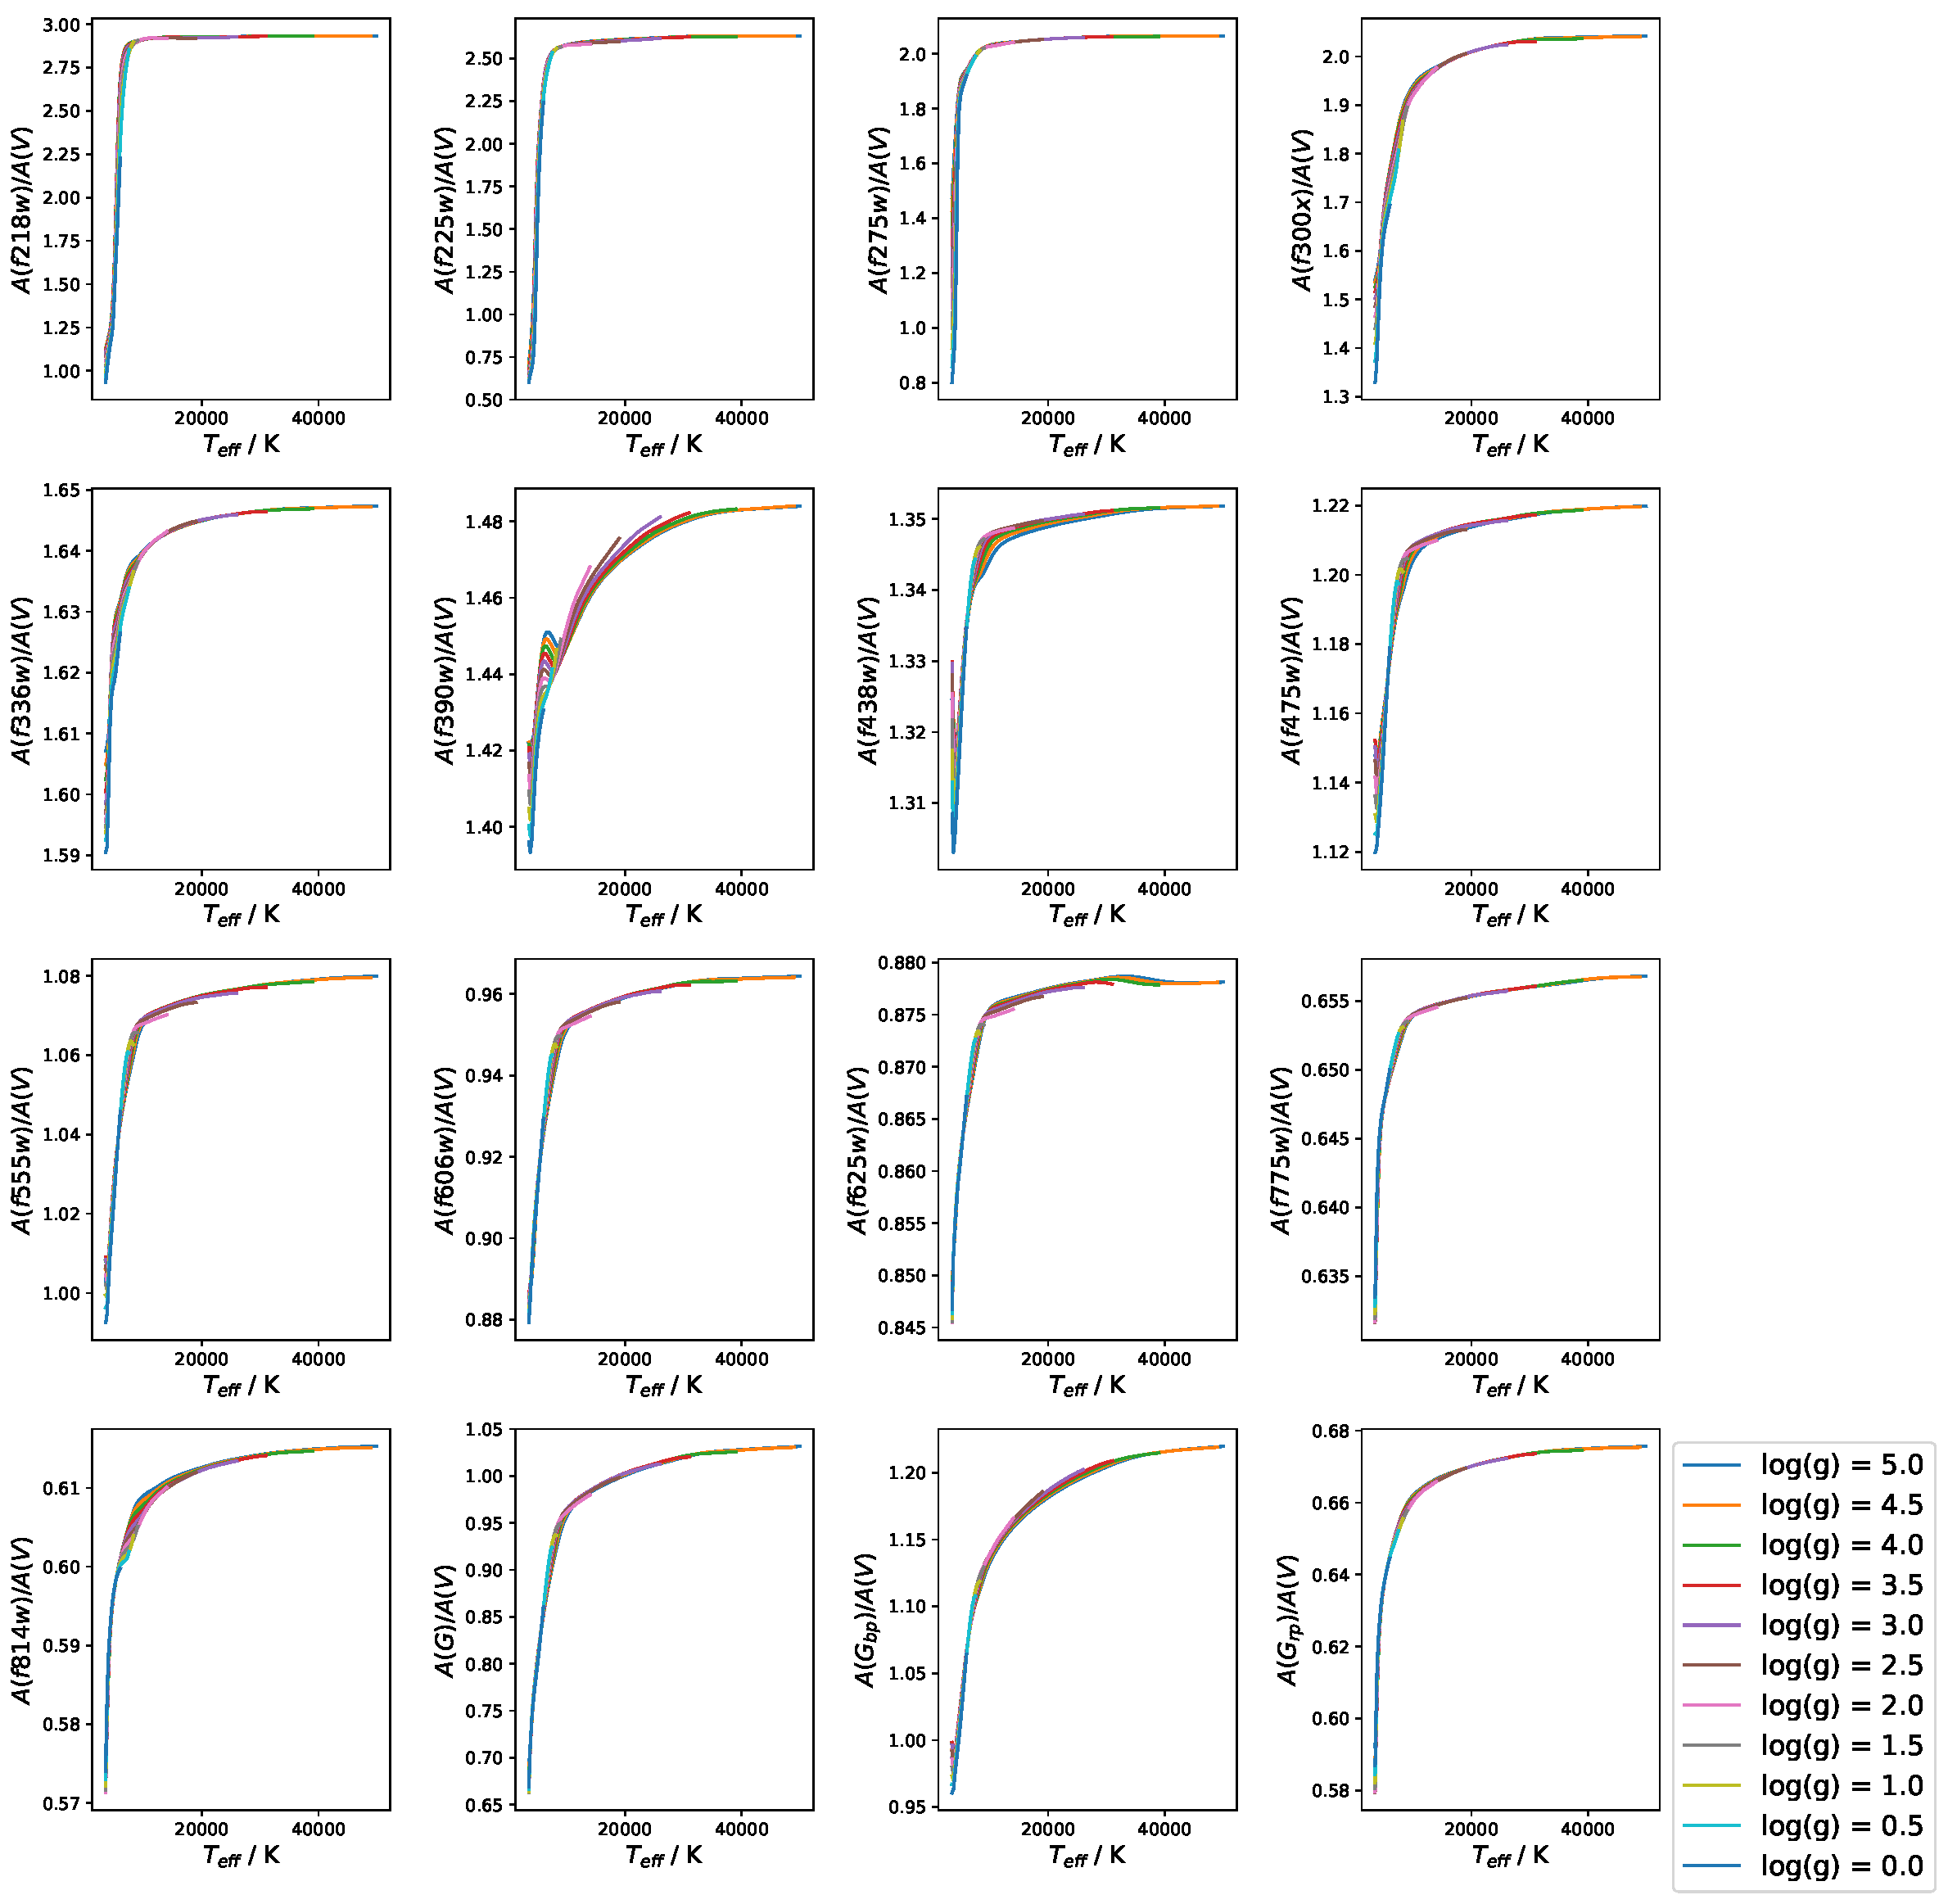
\includegraphics[width=0.85\paperwidth]{../just_full_data/comb/AHub_FeH0p0_just_Teff_plot_lines.pdf}
\caption{Solar-metallicity extinction ratio data for the WFC3 (first 13 panels) and Gaia (last 3) systems, with point-to-point lines connecting datapoints for a fixed log($g$) value.}
\label{just_data_FeH0_WFC3gaia}
\end{center}
\end{figure}

\begin{figure}[h]
\begin{center}
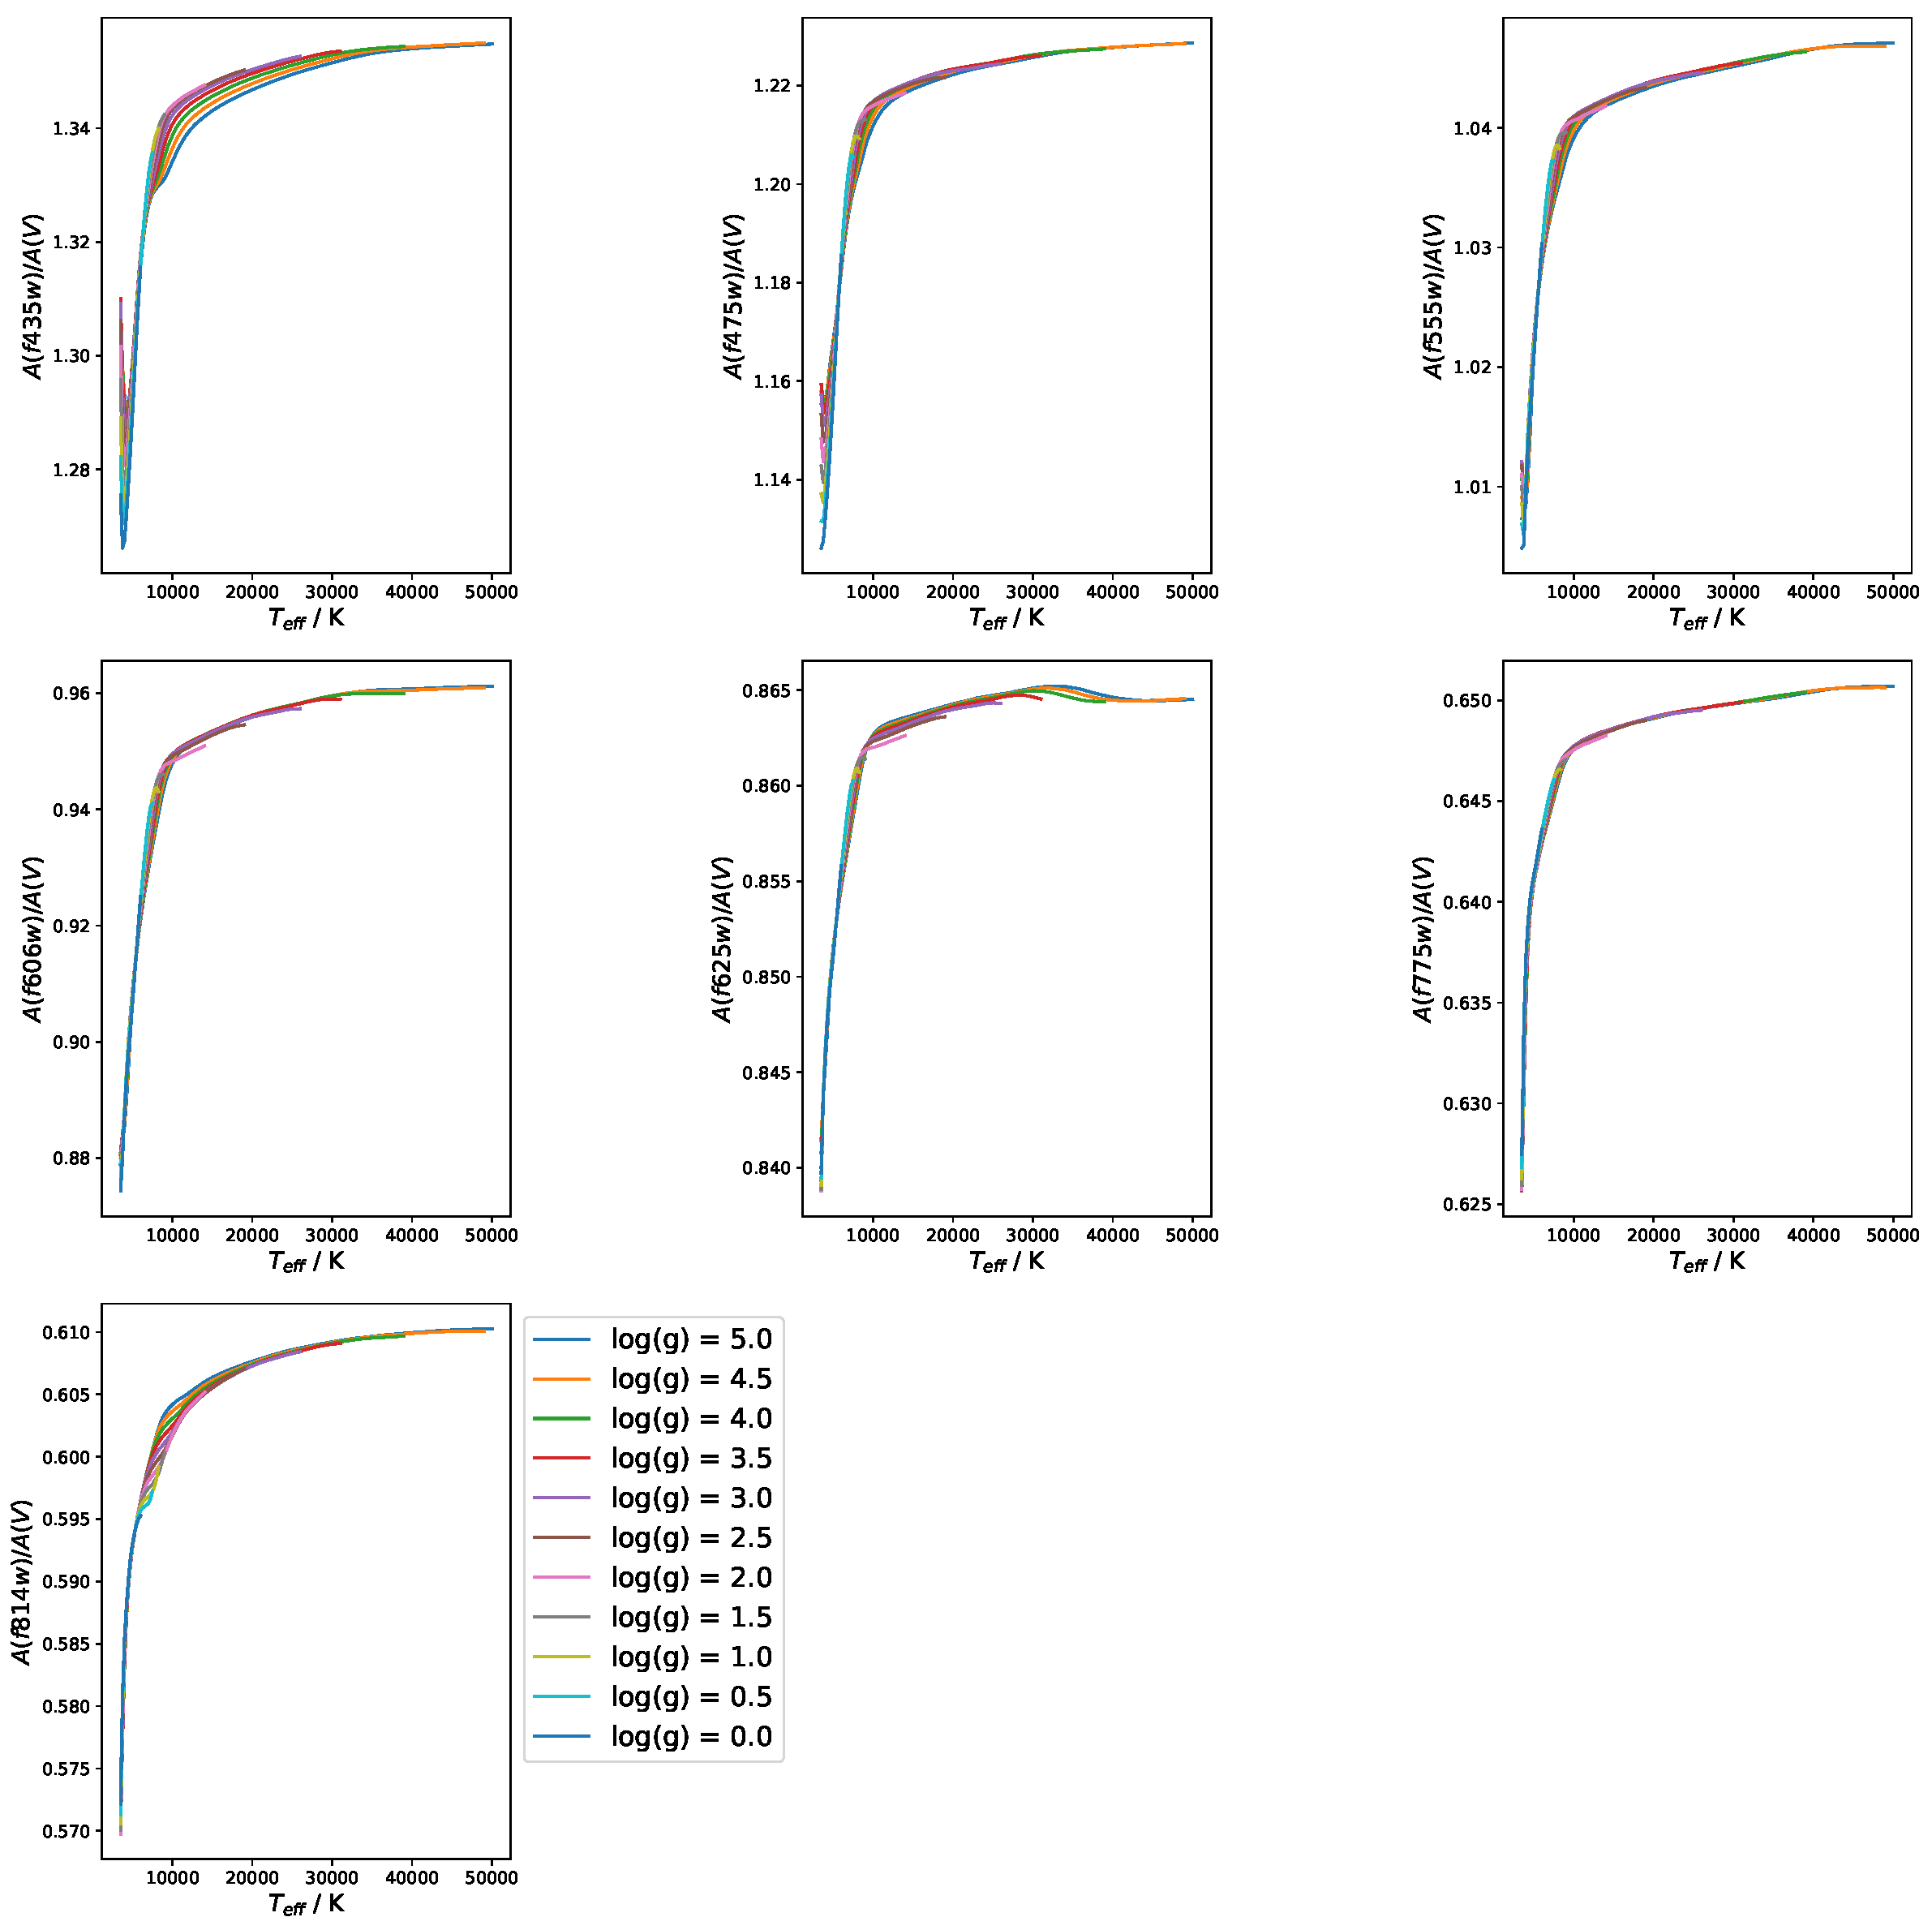
\includegraphics[width=1.0\textwidth]{../just_full_data/ACS/AHub_FeH0p0_just_Teff_plot_lines.pdf}
\caption{Same as Figure \ref{just_data_FeH0_WFC3gaia}, except the filters shown here are for the ACS system.}
\label{just_data_FeH0_ACS}
\end{center}
\end{figure}

A property found in the data for some filters, more pronounced at higher metallicity, is the tendency of the gradient of $A_{X}/A_{V}$ with increasing $T_{\textnormal{eff}}$ to become significantly less positive at the lowest temperatures in the data, typically around 4000K and below. The spread in $A_{X}/A_{V}$ values for different log($g$) is typically about 0.02-0.04, with a linear progression from log($g$) = 5.0 at the lowest end to log($g$) = 0.0 at the highest. In some filters, at the highest metallicity employed ([Fe/H] = 0.5), this phenomenon causes the gradient to invert and become significantly negative, reversing the trend everywhere else in the data, including for the same filters at lower metallicity. Due to the shape of the resulting point-to-point line in these axes, as plotted in both Figures \ref{just_data_FeH0_WFC3gaia} and \ref{just_data_FeH0_ACS}, it has been dubbed the ``tail-flick'' phenomenon. In the same figures, the phenomenon is particularly prominent in the plots for the ACS F435W, WFC3 F438W, F475W (both WFC3 and ACS) and Gaia $G_{\textnormal{bp}}$ filters.\\*

This gradient inversion was ignored as an artefact from the numerical integration required for Equation \ref{BC_extinc}. This was justified on the basis that it is physical infeasible for a cooler star to experience a higher extinction $A_{X}$ than a hotter star for a globally-constant $A_{V}$ value and metallicity, as was assumed for the $A_{X}/A_{V}$ data in this project. Therefore, only data for atmospheres with effective temperatures above those affected by the gradient inversion was used by the algorithm to fit the coefficients of the chosen functions in these filters.\\*

\section{Extinction ratio models} \label{ext_models}

In order to find suitable model functions without running into issues with degeneracy between coefficients in the same function, the relative magnitude of the variations of $A_{X}/A_{V}$ with each of the three stellar parameters became important. This allowed for simple functions expressed solely in terms of $T_{\textnormal{eff}}$, which caused the greatest variations, to be fitted first. The coefficients resulting from the fitting process were then incorporated into the function to form a predicted $A_{X}/A_{V}$ model of $T_{\textnormal{eff}}$. The residuals generated by the subtraction of this predicted model from the original data could then be examined for any significant disagreements between the data and these simple models and for any further variations with log($g$) or [Fe/H]. This allowed functions to be constructed incrementally, with a lower risk of becoming overly complex. Too many coefficients would create errors that were significantly greater in degenerate coefficients than in non-degenerate ones. This would obscure any useful information about the validity of the function form. \\*

The fitting operation for the initial functions of $T_{\textnormal{eff}}$ only was carried out on the dataset for solar metallicity ([Fe/H] = 0.0) ATLAS9 atmospheres and, because it gave the greatest number of $T_{\textnormal{eff}}$ data points, log($g$) = 5.0. Due to the difficulties posed by the tail-flick phenomenon in certain filters, when fitting for $A_{\textnormal{pow}}$ and $A_{\textnormal{exp}}$, the lower $T_{\textnormal{eff}}$ limit for the fitting data was set at 4500K for all filters. This dataset will be referred to as the basic fitting data (BFD). The first functions to be fitted to the BFD had the following forms:

\begin{equation}
A_{\textnormal{pow}} = \left(\frac{A_{X}}{A_{V}}\right)_{\textnormal{pow}}(T_{\textnormal{eff}}) = a (T_{4})^{b} + c
\label{Teff_pow}
\end{equation}

\begin{equation}
A_{\textnormal{exp}} = \left(\frac{A_{X}}{A_{V}}\right)_{\textnormal{exp}} (T_{\textnormal{eff}}) = a \exp(b T_{4}) + c
\label{Teff_exp}
\end{equation}

where $T_{4} = 10^{-4} \times T_{\textnormal{eff}}$. These functions were fitted separately to the BFD for each filter and compared both visually and via the size of the residuals. The most accurate function form was then selected as the final form. The results of this fitting process are detailed, for the cases where the either the $A_{\textnormal{exp}}$ or the $A_{\textnormal{pow}}$ fitting result was sufficiently accurate, in Table \ref{simpfunc_coeffs_table}. The table shows the filters and lists which of the two functions provided the best fit for the relevant data, followed by the respective coefficient values and the associated uncertainties. Due to the fitting data being restricted to atmospheres with $T_{\textnormal{eff}}$ values greater than 4500K, the models could not simply be assumed to apply to cooler atmospheres as well. The final column in Table \ref{simpfunc_coeffs_table} lists the lowest $T_{\textnormal{eff}}$ value for which the given combination of coefficient values is valid at all combinations of surface gravity and metallicity, denoted by $T_{\textnormal{min}}$, together with the maximum deviation of the extinction ratio model from the data, over all stellar atmospheres with $T_{\textnormal{eff}} \geq T_{\textnormal{min}}$, including those not in the BFD (i.e, at non-solar metallicities), in brackets. \\*

For the wide-field WFC3, ACS \citep{2014MNRAS.444..392C} and Gaia \citep{2018MNRAS.479L.102C} filters that were examined in the relevant studies, the opportunity was taken to compare the models for $R_{X} = (A_{X}/E(B-V))$ calculated in those studies, whose basic form is shown in Equation \ref{casagrande_ext_fit}, with the $A_{X}/A_{V}$ data calculated in this project for the same filters. To perform this comparison, it is necessary to define $A_{X}/A_{V}$ explicitly in terms of $R_{X}$. Using the definitions of $R_{X}$ and $R_{V}$, this can be done via the following equation:

\begin{equation}
\frac{A_{X}}{A_{V}} = \frac{R_{X}}{R_{V}} = \frac{R_{X}}{3.1}
\label{convert_Rx_to_Ax}
\end{equation}

The $R_{X}$ models, when modified in this way to produce predictions of $A_{X}/A_{V}$ values, consistently underestimate the $A_{X}/A_{V}$ values listed in the data for atmospheres at log($g$) = 4.0 (the $R_{X}$ models used atmospheric data with log($g$) = 4.1) in this project in almost all filters. However, within the metallicity and temperature ranges for which these $R_{X}$ models are applicable (detailed in Section \ref{empirical}), they remain in agreement with the data to within a $A_{X}/A_{V}$ deviation of 0.03, which is a similar level of accuracy to that achieved by the $A_{X}/A_{V}$ functions produced in this project for the same filters.\\*

There were filters, namely the four WFC3 filters with the shortest central wavelengths (F218W,F225W, F275W and F300X), for whose BFD neither $A_{\textnormal{pow}}$ nor $A_{\textnormal{exp}}$ was able to produce an accurate fit across all combinations of log($g$) and [Fe/H]. For these filters, more intricate functions were sought, including functions with explicit dependences on $g$ and [Fe/H]. Several unsuccessful methods were made before an acceptable function was found for these filters.\\*

The most successful approach for these filters involved plotting all the available $A_{X}/A_{V}$ data for each filter, in all possible 2D and 3D axis combinations, and analysing it visually. The trends seen in the data were analysed to determine both a basic overarching function for the extinction ratio, describing the greatest variations in $T_{\textnormal{eff}}$, and describing the parameters in this function using further mathematical functions (referred to hereafter as ``sub-functions'') within this main function. An example of a sub-function would be a decay coefficient described as a function of log($g$) and [Fe/H].\\*

The details of the final form of the template as a function of each stellar parameter were deduced by fitting a logistic function of $T_{\textnormal{eff}}$ to the $A_{X}/A_{V}$ data for each ([Fe/H],log($g$)) combination. This was decided on the basis that $A_{\textnormal{exp}}$ had been superior to $A_{\textnormal{pow}}$ in describing the data for these particular filters and because the low-$T_{\textnormal{eff}}$ change in gradient appeared to be more significant than for other filters. Furthermore, the gradient was not inverted, as can be seen in Figure \ref{just_data_FeH0_WFC3gaia}, thus avoiding any tail-flicks. Of particular importance was the additional fact that the $T_{\textnormal{eff}}$ gradient in the region between the shallow low-$T_{\textnormal{eff}}$ gradient and the plateau appears to lead to an asymptote at lower stellar effective temperatures, if the shallower low-$T_{\textnormal{eff}}$ gradient is ignored when constructing and fitting a function (as was done for both $A_{\textnormal{exp}}$ and $A_{\textnormal{pow}}$). In these four filters, this steep gradient was found to cause functions such as $A_{\textnormal{exp}}$ and $A_{\textnormal{pow}}$ to predict negative values of the extinction ratio at $T_{\textnormal{eff}}$ values that were still above the lowest values derived from observations of cool stars (excluding brown dwarfs). This issue is resolved by the logistic function's property of converging to a constant value for both high and low values of $T_{\textnormal{eff}}$. Therefore, for these filters, the data to which the functions were fitted encompassed all available $T_{\textnormal{eff}}$ values down to the ATLAS9 minimum of 3500K. For a general logistic function in $T_{\textnormal{eff}}$ (whose basic form is shown in Equation \ref{A_logis_UV}), there are four key parameters:

\begin{itemize}
\item The global maximum value, denoted in this case by $A_{max}$;
\item The global minimum value, $A_{min}$;
\item The exponential decay coefficient, $k$;
\item The $T_{\textnormal{eff}}$-coordinate of the sigmoid midpoint, in this case $T_{\textnormal{0}}$.
\end{itemize}

It was confirmed that this logistic function of $T_{\textnormal{eff}}$ could describe the $A_{X}/A_{V}$ variations accurately in each filter for every combination of atmospheric log($g$) and [Fe/H] values, using the four parameters listed above. This was done numerically by fitting the logistic function to the $A_{X}/A_{V}$ data for each (log($g$),[Fe/H]) combination individually. The values for the coefficients produced for each of these fits were tabulated along with the log($g$) and [Fe/H] values of their respective datasets. This table was then analysed for trends in the coefficient values as log($g$) and [Fe/H] were varied. This allowed for the incremental construction, where necessary, of sub-functions to describe the parameters of the main logistic function, itemised above, in terms of log($g$) and [Fe/H].\\*

Many different forms, of varying complexity, were tested for these sub-functions. With each new form, the sub-functions were incorporated into the main $T_{\textnormal{eff}}$-logistic function. In some cases, sub-functions with explicit $T_{\textnormal{eff}}$ dependences were included. The resulting function was then subjected to a fit on the entire $A_{X}/A_{V}$ dataset, covering the entire ($T_{\textnormal{eff}}$,  log($g$), [Fe/H]) parameter space available. The suitability of each function was influenced by both the size of the $A_{X}/A_{V}$ residuals and on the relative errors on the coefficients resulting from the fit. The importance of the latter was due to multiple factors:

\begin{itemize}
\item the possibility of degeneracies between coefficients being overlooked during the construction of either the sub-functions, the overall function or both, which would result in anomalously high errors for the relevant coefficients;
\item the possible occurrence of near-zero best-fit value for a given coefficient with a high associated error, indicating that the coefficient was describing a trend not actually present in the data and that, therefore, the overall function was overly complex;
\item the danger of coefficient values not departing from the initial value with zero error, indicating that, for that coefficient, the algorithm was unable to achieve convergence, even after a very large number of iterations.
\end{itemize}

The best form for the sub-functions were found to be simple functions of log($g$) and [Fe/H], independent of $T_{\textnormal{eff}}$ variations. This allowed them to be used as the definitions of $T_{0}$ and $k$, as shown in Equations \ref{T0_eq} and \ref{decay_const_eq}, respectively. The overall function, $A_{\textnormal{logis}}$, is therefore sensitive to all three input stellar atmosphere parameters, with effective temperature having the greatest effect and the other parameters having much smaller but still significant effects, with the relative magnitudes dependent on the values of the associated coefficients.\\*

This final form of $A_{\textnormal{logis}}$ was able to accurately reproduce the behaviour of almost the entire dataset. The coefficients for Equations \ref{T0_eq}-\ref{A_logis_UV} are given in Table \ref{UV_coeffs_table}. \\*

\begin{align}
T_{\textnormal{0}} &= a\log(g) + b\left(\frac{\left[\textnormal{Fe/H}\right]}{\left|\left[\textnormal{Fe/H}\right]\right|^{1/2}}\right) + c \label{T0_eq}\\
k &= d\log(g) + e\left[\textnormal{Fe/H}\right] + f \label{decay_const_eq}\\
A_{\textnormal{logis}} = \left(\frac{A_{X}}{A_{V}}\right)_{\textnormal{logis}}(T_{\textnormal{eff}},g,\left[\textnormal{Fe/H}\right]) &= \frac{(A_{max}-A_{min})}{( 1 + \exp{(-10^{-4} k(T_{\textnormal{eff}}-T_{\textnormal{0}})) ) )}} + A_{min} \label{A_logis_UV}
\end{align}


\begin{table}
\begin{center}
\resizebox{\textwidth}{!}{\begin{tabular}{ccccccc}
\hline
System & Filter &  Function & & Coefficients & & $T_{\textnormal{min}}$ / K \\
 & & ($A_{\textnormal{pow}}$ or $A_{\textnormal{exp}}$) & $a$ & $b$ & $c$ & (global maximum error margin) \\
\hline
& F435W & exp & -0.1436$\pm$0.0310 & -2.159$\pm$0.360 & 1.352$\pm$0.002 & 3500(0.03) \\
& F475W & exp & -0.2137$\pm$0.0469 & -2.660$\pm$0.380 & 1.226$\pm$0.002 & 4000(0.03) \\
& F555W & exp & -0.0914$\pm$0.0476 & -2.677$\pm$0.901 & 1.045$\pm$0.002 & 3500(0.01) \\
ACS & F606W & exp & -0.2183$\pm$0.0554 & -2.867$\pm$0.445 & 0.959$\pm$0.002 & 3500(0.01) \\
& F625W & exp & -0.0719$\pm$0.0798 & -3.332$\pm$2.000 & 0.865$\pm$0.002 & 3500(0.01) \\
& F775W & pow & -0.0035$\pm$0.0042 & -1.488$\pm$1.541 & 0.651$\pm$0.003 & 3500(0.01) \\
& F814W & pow & -0.0070$\pm$0.0046 & -1.374$\pm$0.830 & 0.611$\pm$0.003 & 3750(0.02) \\ \hline

& F336W & pow & -0.0074$\pm$0.0041 & -1.525$\pm$0.727 & 1.648$\pm$0.003 & 3500(0.03) \\
& F390W & exp & -0.0695$\pm$0.0057 & -0.644$\pm$0.177 & 1.489$\pm$0.005 & 4500(0.04) \\
& F438W & exp & -0.1132$\pm$0.0658 & -3.084$\pm$1.032 & 1.350$\pm$0.002 & 3750(0.02) \\
& F475W & pow & -0.0179$\pm$0.0037 & -1.718$\pm$0.275 & 1.220$\pm$0.003 & 4000(0.02) \\
WFC3 & F555W & pow & -0.0138$\pm$0.0033 & -1.887$\pm$0.333 & 1.080$\pm$0.003 & 3750(0.02) \\
& F606W & exp & -0.2131$\pm$0.0559 & -2.879$\pm$0.460 & 0.962$\pm$0.002 & 3500(0.02) \\
& F625W & pow & -0.0042$\pm$0.0031 & -2.063$\pm$1.025 & 0.879$\pm$0.002 & 3500(0.01) \\
& F775W & pow & -0.0033$\pm$0.0041 & -1.529$\pm$1.634 & 0.657$\pm$0.003 & 3750(0.01) \\
& F814W & pow & -0.0071$\pm$0.0046 & -1.391$\pm$0.803 & 0.616$\pm$0.004 & 4000(0.01) \\ \hline

& G & pow & -0.0888$\pm$0.0045 & -1.402$\pm$0.064 & 1.040$\pm$0.004 & 4000(0.02) \\
Gaia & G\textsubscript{bp} & pow & -0.1150$\pm$0.0081 & -0.900$\pm$0.070 & 1.247$\pm$0.007 & 3750(0.03) \\
& G\textsubscript{rp} & pow & -0.0159$\pm$0.0047 & -1.352$\pm$0.368 & 0.677$\pm$0.004 & 3750(0.02) \\ \hline

\end{tabular}}
\caption{Coefficient values produced for each filter via $A_{\textnormal{exp}}$ or $A_{\textnormal{pow}}$ fitting, as appropriately labelled. Any filters missing from this table are those with data that could not be accurately fitted using either function. The errors are calculated using an acceptable 1$\sigma$ margin, $\Delta(A_{X}/A_{V})$, of 0.01. The final column displays the lowest effective temperature, including for atmospheres outside the BFD, for which the given model and coefficients were able to describe the $A_{X}/A_{V}$ data across all values of log($g$) and [Fe/H].}
\label{simpfunc_coeffs_table}
\end{center}
\end{table}

\begin{table}
\begin{center}
\begin{tabular}{ccccc}
\hline
\multirow{2}{*}{Coefficient} & \multicolumn{4}{c}{Filter} \\
 & F218W & F225W & F275W & F300X \\
\hline
$a$ & -120.9$\pm$4.1 & -97.21$\pm$3.85 & -239.0$\pm$12.0 & -302.1$\pm$45.0 \\
$b$ & 467.6$\pm$7.9 & 357.2$\pm$7.9 & 236.0$\pm$20.4 & 350$\pm$125 \\
$c$ & 5673$\pm$16 & 4967$\pm$22 & 4161$\pm$79 & 4270$\pm$913 \\
$d$ & 1.435$\pm$0.209 & -0.174$\pm$0.136 & -2.117$\pm$0.326 & -0.176$\pm$0.087 \\
$e$ & -3.211$\pm$0.382 & -2.691$\pm$0.256  & -2.140$\pm$0.445 & -0.352$\pm$0.115 \\
$f$ & 19.19$\pm$0.62 & 18.62$\pm$0.55  & 22.20$\pm$1.48 & 4.315$\pm$0.529 \\
$A_{min}$ & 1.026$\pm$0.012 & 0.337$\pm$0.028 & 0.409$\pm$0.113 & 1.000$\pm$0.199 \\
$A_{max}$ & 2.909$\pm$0.003 & 2.581$\pm$0.003 & 2.030$\pm$0.003 & 2.015$\pm$0.004 \\
\hline
Max. deviation in $A_{X}/A_{V}$ & 0.25 & 0.3 & 0.2 & 0.15 \\
%($T_{\textnormal{eff}}$ / K, & & & None & None \\
%log($g$) / dex, & & & None & None \\
%$\textnormal{[Fe/H]}$) & & & None & None \\
%exceptions & & & & \\
\hline
\end{tabular}
\caption{Coefficient values for the non-trivial $A_{X}/A_{V}$ function $A_{\textnormal{logis}}$, described in Equations \ref{T0_eq}-\ref{A_logis_UV}, produced by fitting to UV filter data with The errors are calculated using an acceptable 1$\sigma$ margin, $\Delta(A_{X}/A_{V})$, of 0.1. The bottom row represents the maximum deviation from the data across the entire ($T_{\textnormal{eff}}$, log($g$), [Fe/H]) parameter space. All results are valid down to $T_{\textnormal{eff}}$ = 3500 K.}
\label{UV_coeffs_table}
\end{center}
\end{table}

All the functions are consistent with the general trends predicted by the physics in stellar atmospheres, since the effective temperature has the greatest effect upon the value of $A_{X}/A_{V}$, with relatively minor effects due to spectral absorption lines, via surface gravity and metallicity. In general stars with higher effective temperatures (and consequently stronger and bluer flux spectra) experience higher $A_{X}/A_{V}$ values in all filters than stars with low effective temperatures. The maximum $A_{X}/A_{V}$ value in a given filter decreases as the filter's central wavelength increases. This is expected for black-body analogues (see Equation \ref{planck_bb} and Figure \ref{planck_curve}). Both trends are also consistent with the known short-wavelength preference of physical mechanisms causing interstellar extinction.\\*

In summary, these functions are sufficiently accurate to replicate the results that would be obtained by using a combination of stellar atmosphere data tables and interpolations between the ($T_{\textnormal{eff}}$, log($g$), [Fe/H]) points in the tables. The accuracy of these relatively simple functions is important because the $A_{X}/A_{V}$ dataset for each filter is now reduced to a much smaller number of degrees of freedom, equal to the number of coefficients in the relevant function. The input parameters ($T_{\textnormal{eff}}$, log($g$) and [Fe/H]) are required regardless of whether interpolation of the tables of $A_{X}/A_{V}$ data or the functions are being employed, and so they make no difference in comparing the information complexity of the tables versus the functions.\\*


\section{Effect on isochrones} \label{result_CMDs}
Once the $A_{X}/A_{V}$ functions and the values of their associated coefficients were produced, the effect of using these functions to model extinction in CMDs for stellar populations was studied at a given isochrone age and compared with the effect of the standard method of using constant $A_{X}/A_{V}$ values for isochrones of similar ages in the same CMDs. During this comparison of the methods, particular focus was given to any differences in the CMD position of the MSTO for a given isochrone age and differences in age estimates for a given MSTO position.  \\*

To be able to apply extinction ratios calculated using the functions derived in the previous section to the model stars which constitute the BaSTI isochrones, the models' log($g$) values first had to be explicitly determined. The equations detailed in Section \ref{isoc_fit} were applied to the BaSTI data to do this. The $A_{X}/A_{V}$ functions created in this project could then be applied to the resulting data tables. \\*

When calculating the fixed-extinction $A_{X}/A_{V}$ values to be applied to a given isochrone, the metallicity of the isochrone first had to be accounted for, particularly for UV filters. Therefore, the $A_{X}/A_{V}$ value chosen was taken from the ATLAS9 model whose metallicity best matched that of the isochrone. This ATLAS9 value will be denoted [Fe/H]$_{CM}$, where `$CM$' stands for `closest matching'. The first value was equal to $(A_{X}/A_{V})_{plat} = (A_{X}/A_{V})(T_{\textnormal{eff}} = 50,000\textnormal{K},\log(g) = 5.0,\textnormal{[Fe/H]}_{CM})$, and the second was equal to $(A_{X}/A_{V})_{MS} = (A_{X}/A_{V})(T_{\textnormal{eff}} = 5,000\textnormal{K},\log(g) = 5.0,\textnormal{[Fe/H]}_{CM})$. This was done to reflect the fact that, for the first case, the assumption of a constant extinction value is valid in the plateau region and, for the second, the fact that, given the position of the MSTO in terms of stellar $T_{\textnormal{eff}}$ values, it would be more prudent to ensure that the upper main sequences below the MSTO resulting from both extinction-calculation methods to coincide in the CMD, making it easier to see any disagreements in the turn-off ages. For each of these plots, $A_{V}$ was fixed at a value of 1.0.\\*

In each of the CMDs, the extinction ratio functions have been applied to a solar-metallicity ([Fe/H] = 0), 500 Myr isochrone, which is shown as a solid orange line. A fixed extinction ratio has been applied to three solar-metallicity isochrones with ages of 400 (solid green), 500 (solid blue) and 600 (solid red) Myr, respectively. A solar-metallicity, 500 Myr isochrone with zero extinction is added for illustration purposes as a solid purple line.\\*

\subsection{ACS} \label{ACS_isoc}
The F435W-(F435W-F814W) CMD was chosen for the ACS. This CMD is useful as it pairs the bluest and reddest wide-field filters for the ACS in its colour index, which is the index most likely to distinguish between objects in a given dataset with a large range of effective temperatures, making it useful for modelling the main sequence and MSTO, the two most important CMD components for calculating cluster isochrone ages. This CMD corresponds, by design, to the pre-existing Johnson-Cousins $B$-($B-I$) CMD \citep{2005PASP..117.1049S}, which allows direct comparison of observed data with archive data obtained before the creation of the ACS filters.\\*

\begin{figure}[h]
\begin{center}
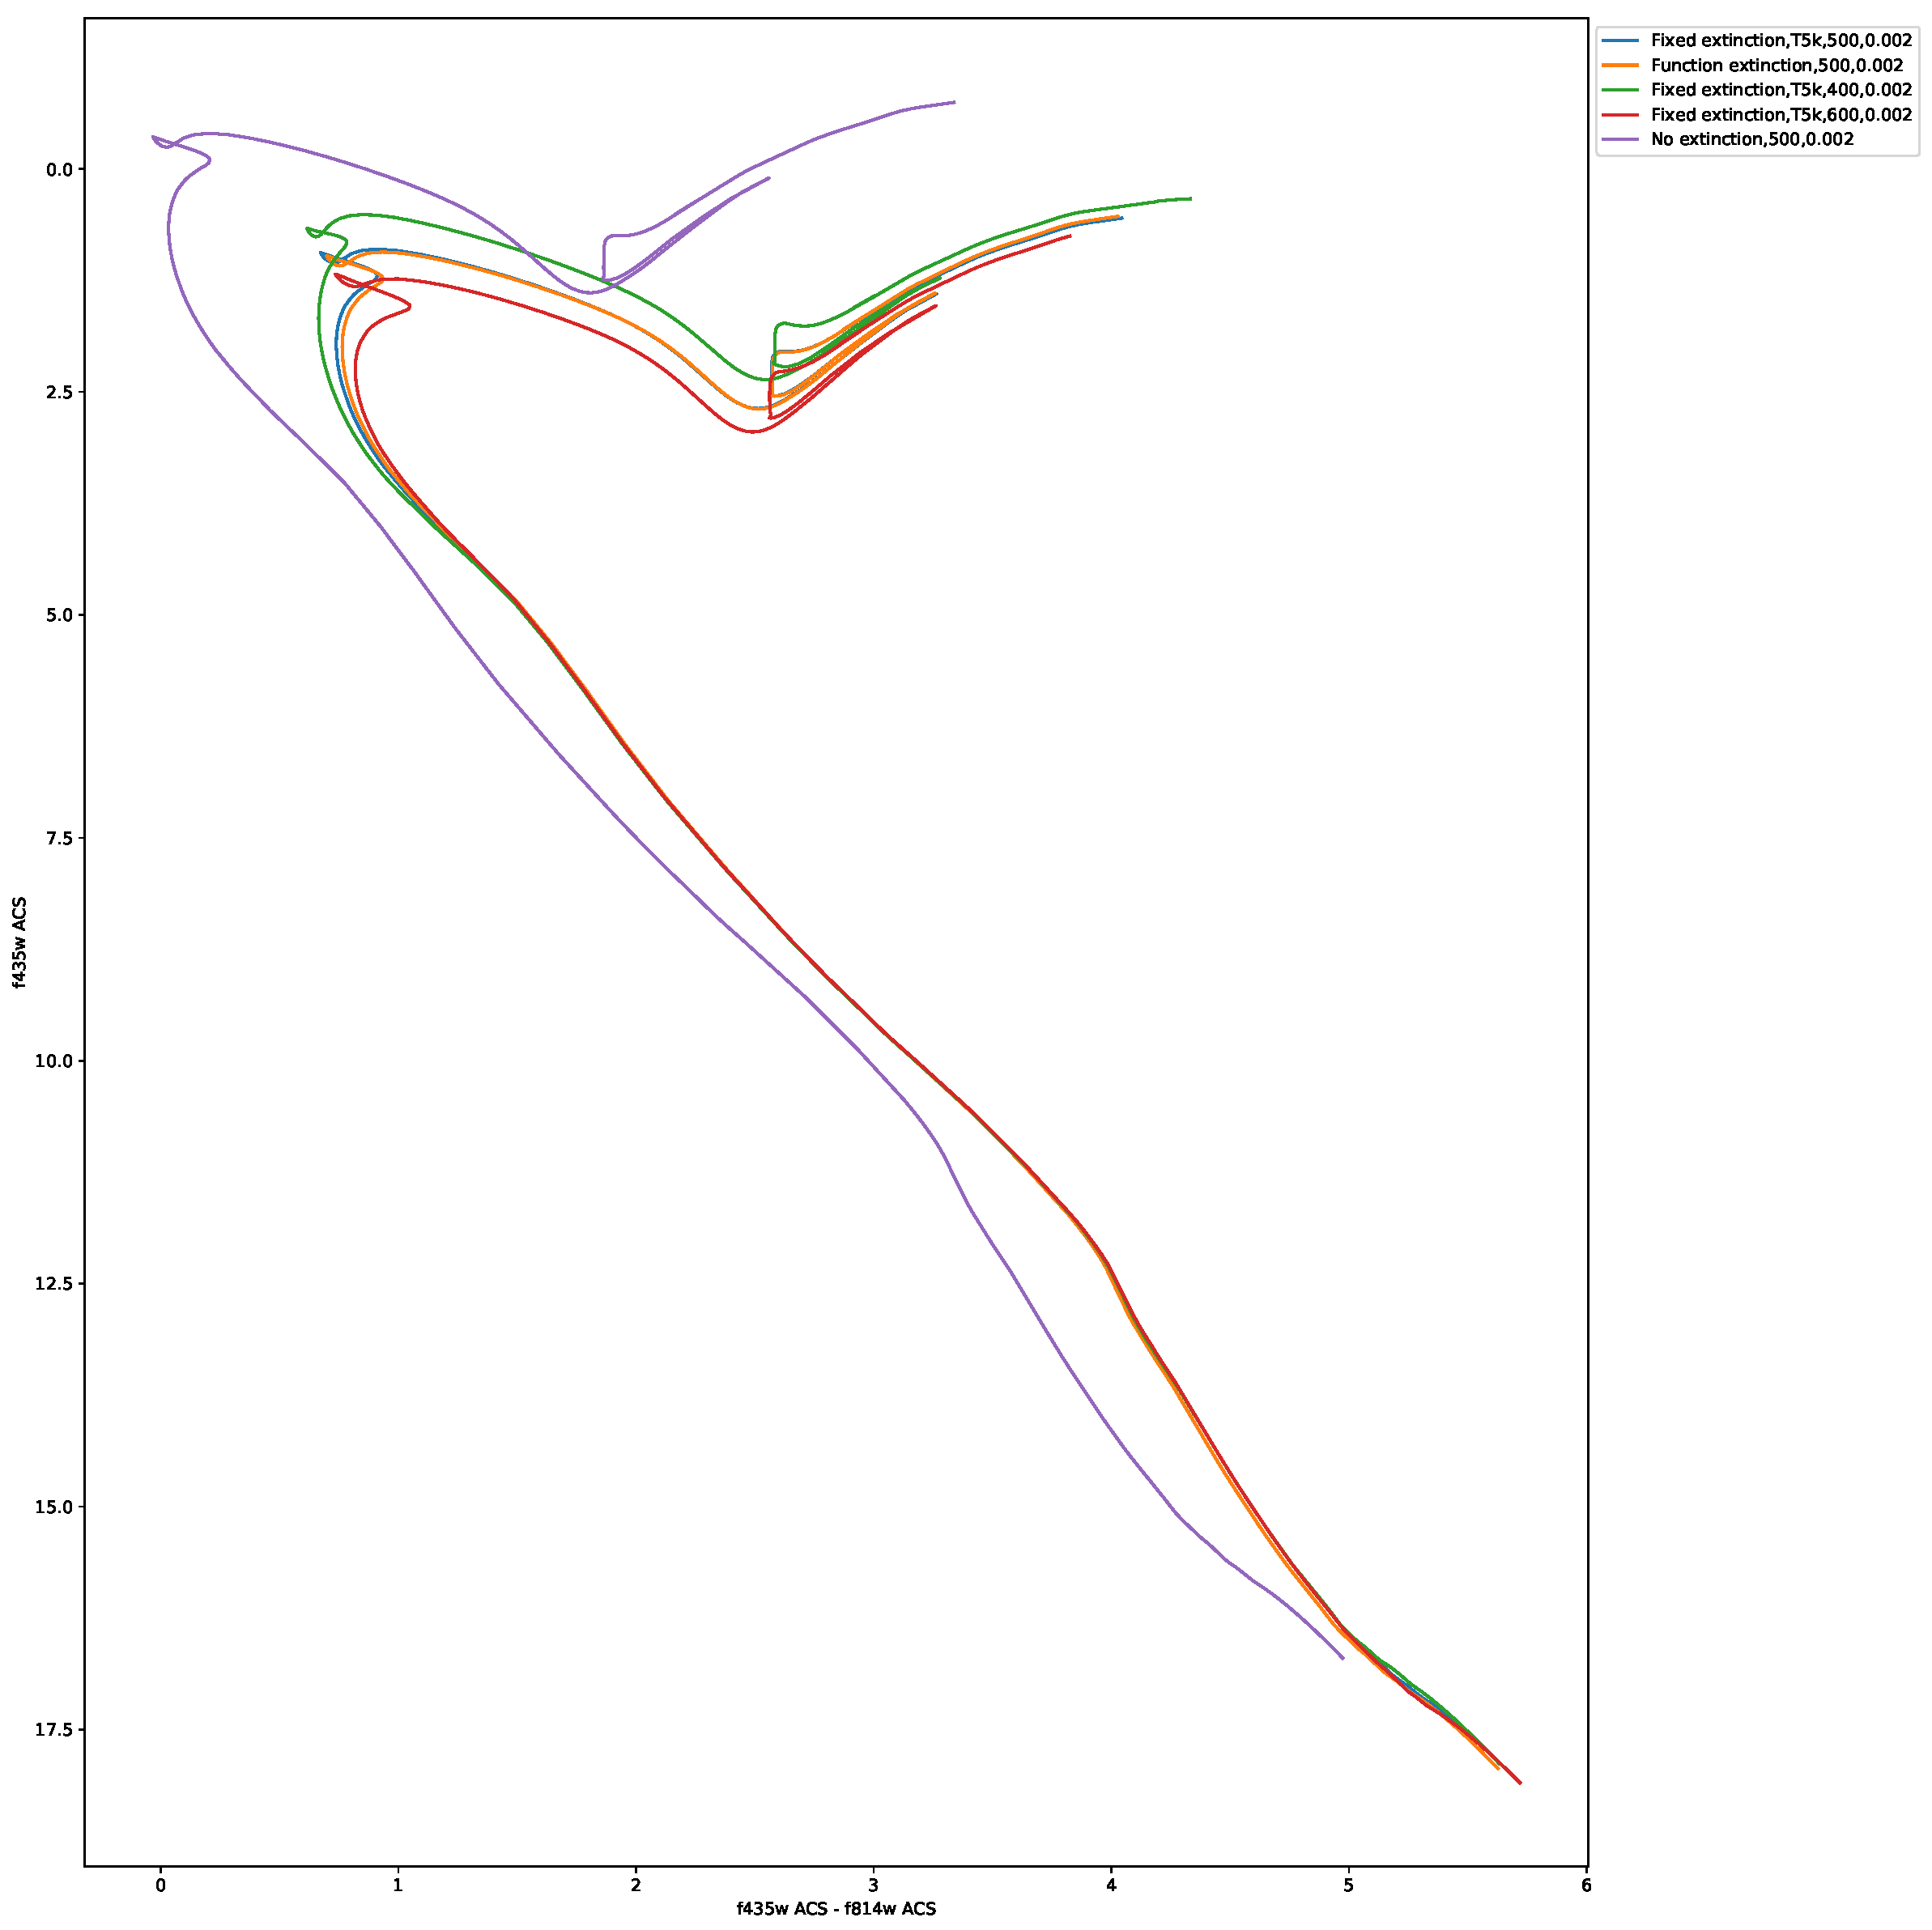
\includegraphics[width=1.0\textwidth]{../basti_isochrones_10_13Gyr/Extinction_T5k_FeH0fix_func_f435wACS_f435wACSmf814wACS_500_400_600_Myr_FeH_0p002_ref_noext_Av_1p0.pdf}
\caption{ACS F435W-(F435W-F814W) CMD with a fixed extinction ratio equal to $(A_{X}/A_{V})_{MS}$ for each filter}
\label{acs_isoc_T5k}
\end{center}
\end{figure}

\begin{figure}[h]
\begin{center}
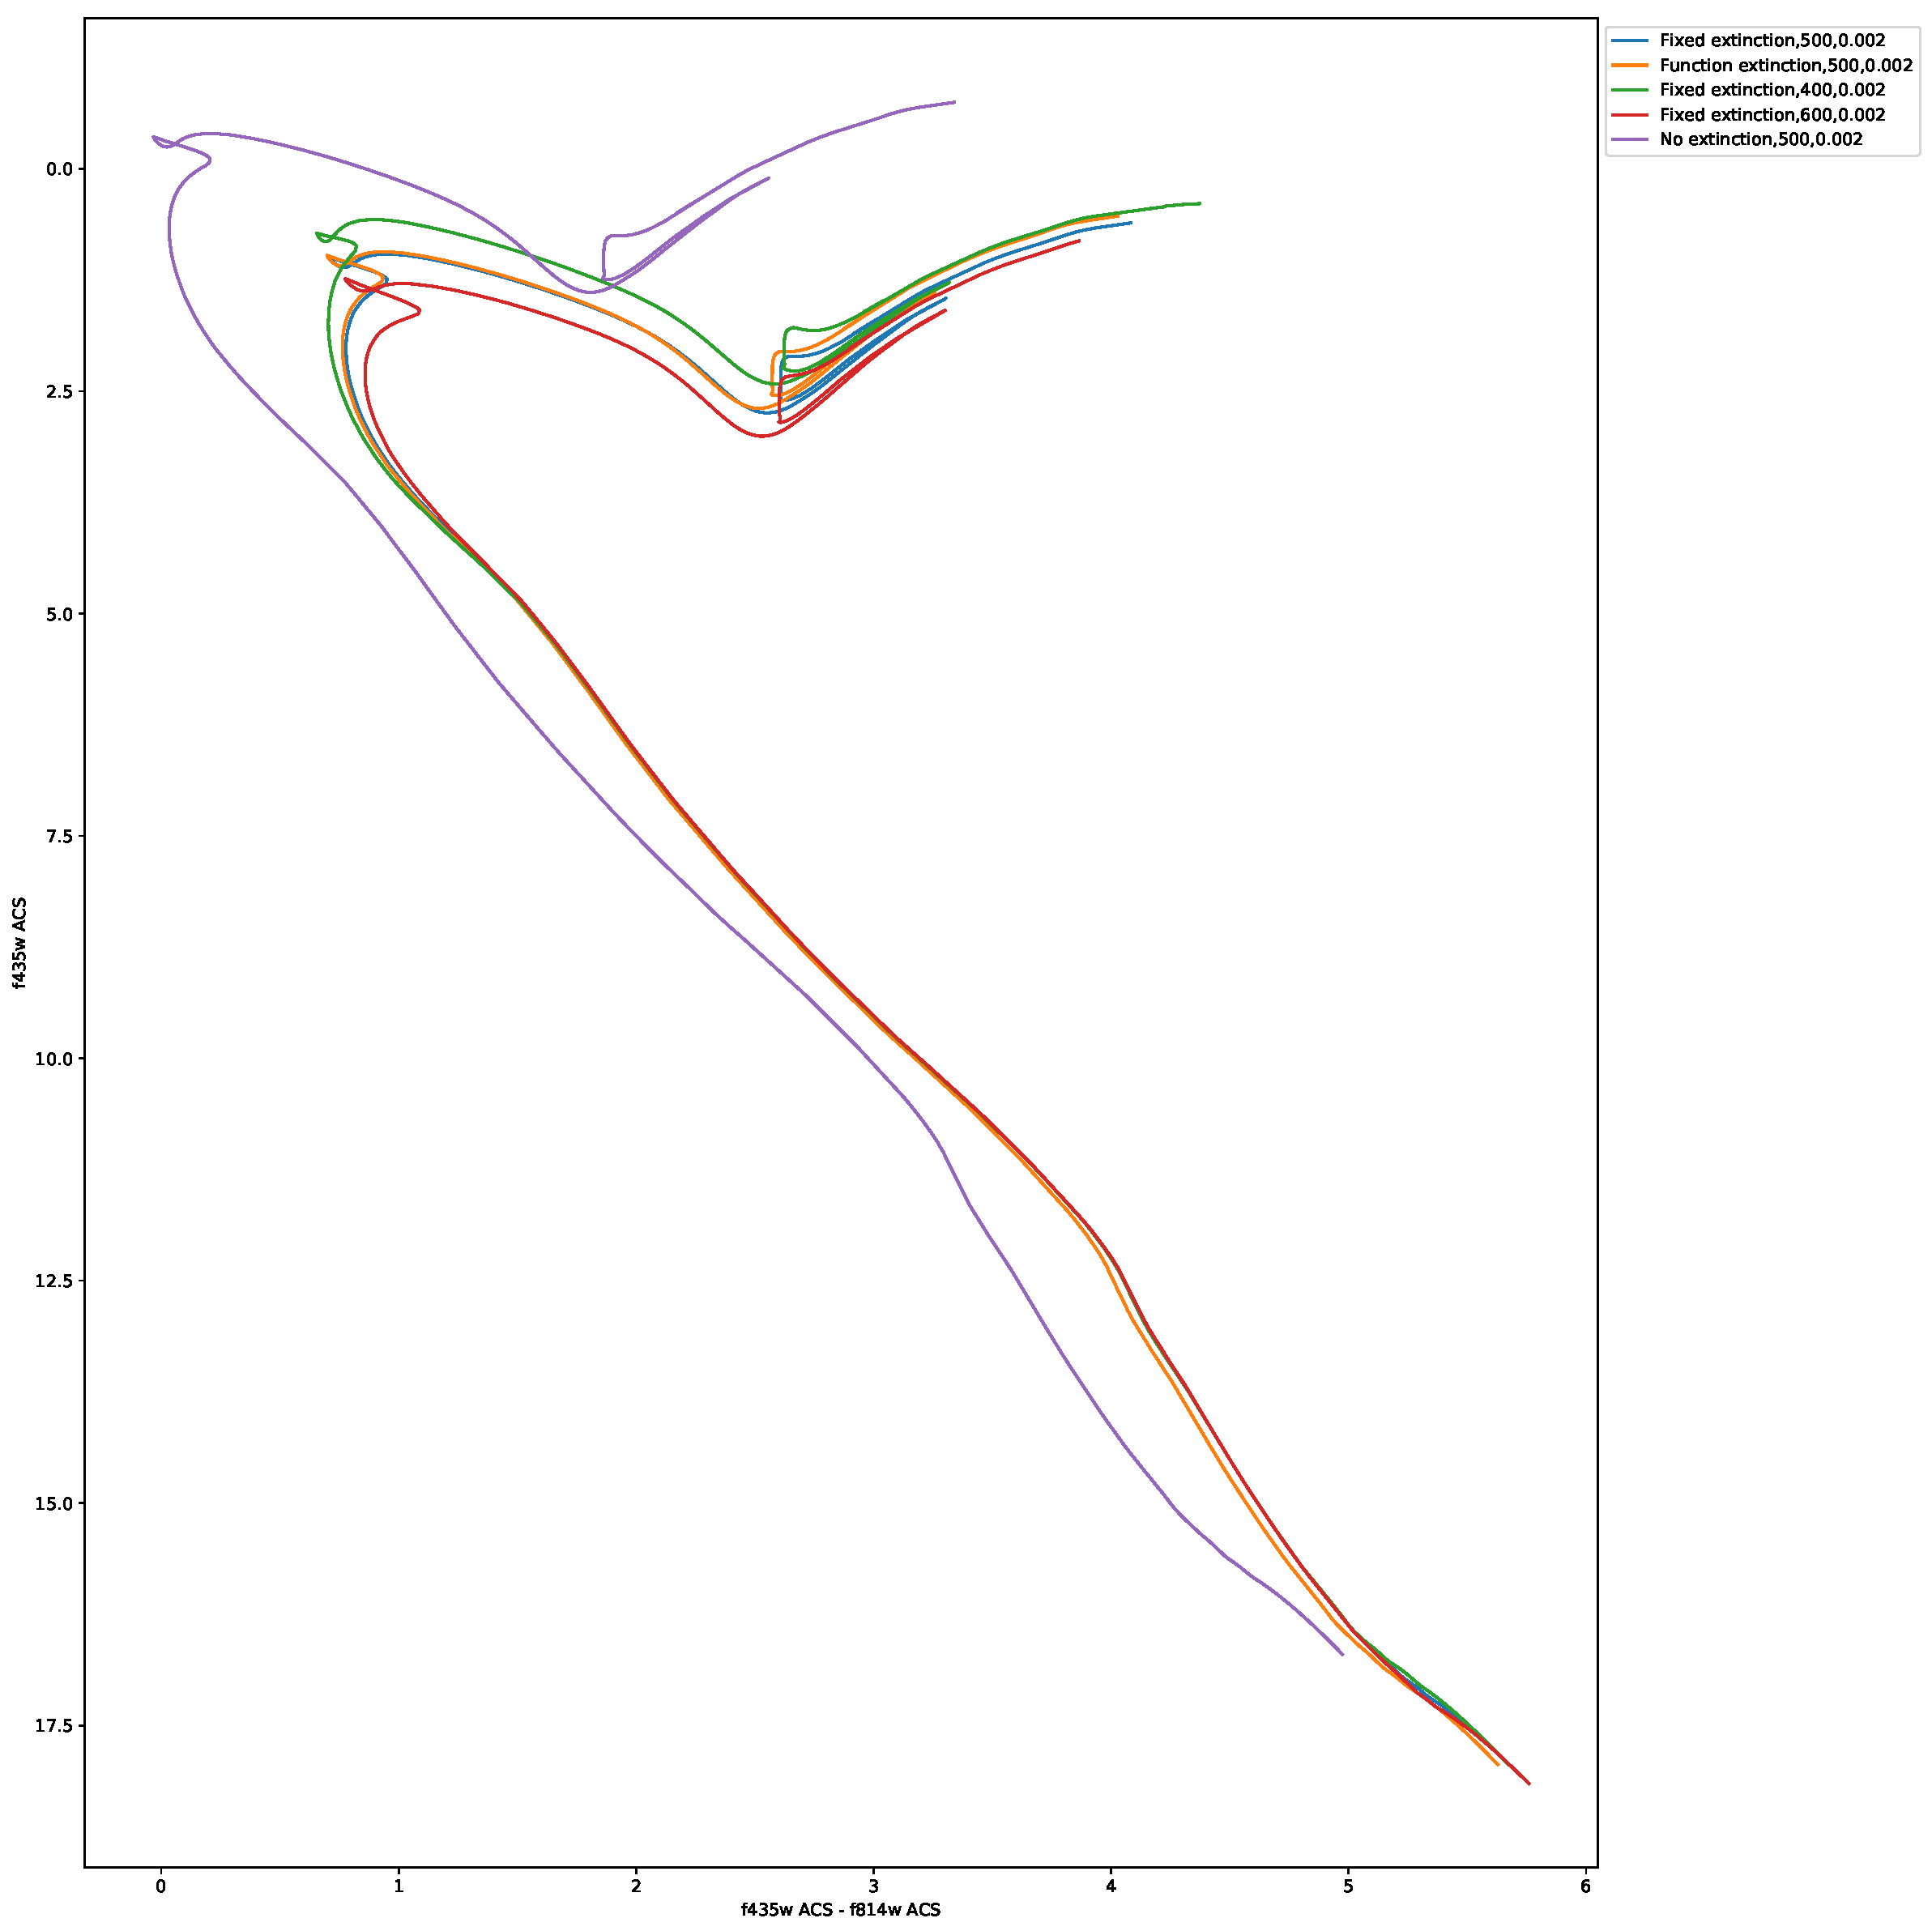
\includegraphics[width=1.0\textwidth]{../basti_isochrones_10_13Gyr/Extinction_T50k_FeH0fix_func_f435wACS_f435wACSmf814wACS_500_400_600_Myr_FeH_0p002_ref_noext_Av_1p0.pdf}
\caption{ACS F435W-(F435W-F814W) CMD with a fixed extinction ratio equal to $(A_{X}/A_{V})_{plat}$ for each filter}
\label{acs_isoc_T50k}
\end{center}
\end{figure}

It can be seen in Figure \ref{acs_isoc_T5k}, by comparing the position of the blue and orange isochrones, that the impact of changing between the FBER and fixed-extinction methods in this CMD is insignificant. Although there are some larger differences in the position of the isochrone in the post-sub-giant branch (SGB) evolutionary stages, this is irrelevant when determining the isochrone age of an observed stellar population.\\*

The result of using $(A_{X}/A_{V})_{plat}$ is not significantly different from that of using $(A_{X}/A_{V})_{MS}$ for this CMD. By comparing Figures \ref{acs_isoc_T5k} and \ref{acs_isoc_T50k}, it is clear that any changes in $A_{X}/A_{V}$ values in the F435W and F814W ACS filters at different temperatures (see Figure \ref{just_data_FeH0_ACS}) are insignificant in the context of these isochrones.\\*

\subsection{WFC3} \label{WFC3_isoc}

Two different CMDs were chosen whose filters are part of the WFC3 system. The first is the F555W-(F555W-F814W) CMD. This CMD pairs a wide yellow filter (F555W) with the WFC3's reddest IR wide-field filter. This CMD mimics the pre-existing and widely-used Johnson-Cousins $V$-($V-I$) CMD \citep{2014wfc..rept...16S}, which allows direct comparison of observed data with archive data obtained before the creation of the WFC3 filters.\\*

As with the previous ACS CMD, this CMD shows no significant changes in isochrone position resulting from either employing a FBER model or changing the extinction ratio value used for the fixed-value extinction model from $(A_{X}/A_{V})_{plat}$ to $(A_{X}/A_{V})_{MS}$ or vice versa.\\*

\begin{figure}[h]
\begin{center}
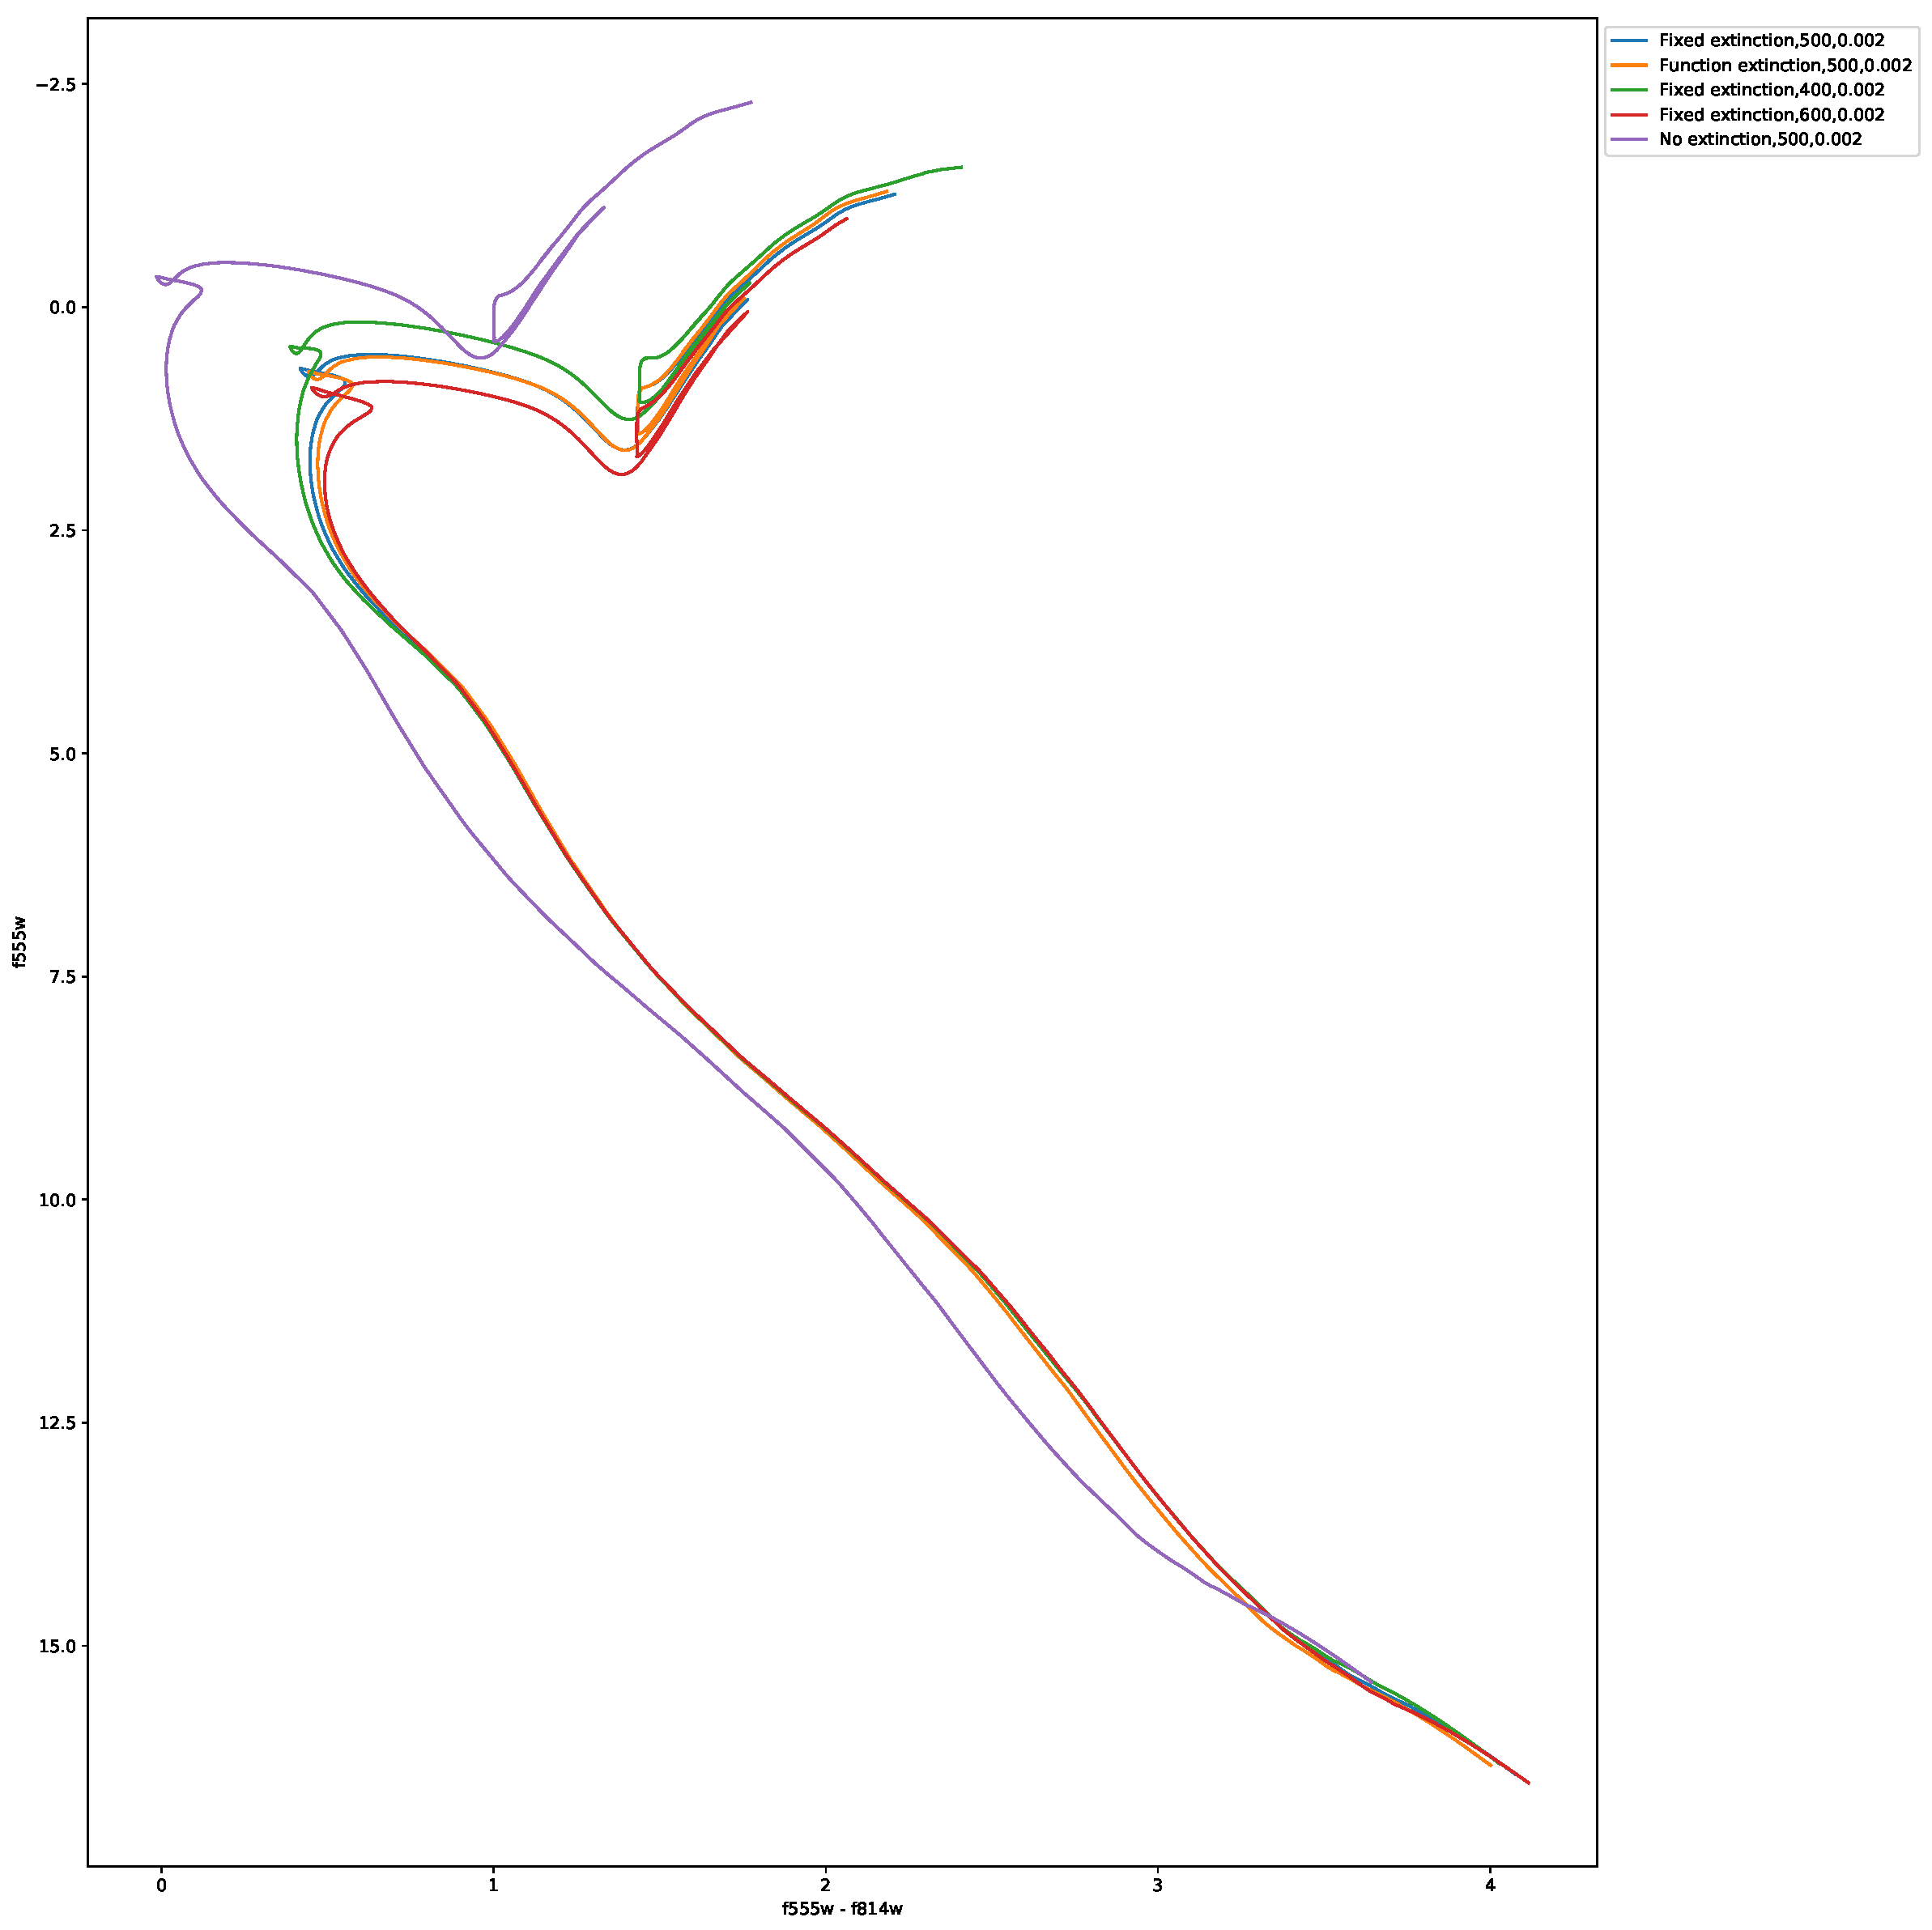
\includegraphics[width=1.0\textwidth]{../basti_isochrones_10_13Gyr/Extinction_T5k_FeH0fix_func_f555w_f555wmf814w_500_400_600_Myr_FeH_0p002_ref_noext_Av_1p0.pdf}
\caption{WFC3 F555W-(F555W-F814W) CMD with a fixed extinction value equal to $(A_{X}/A_{V})_{MS}$ for each filter}
\label{wfc3_isoc1_T5k}
\end{center}
\end{figure}

\begin{figure}[h]
\begin{center}
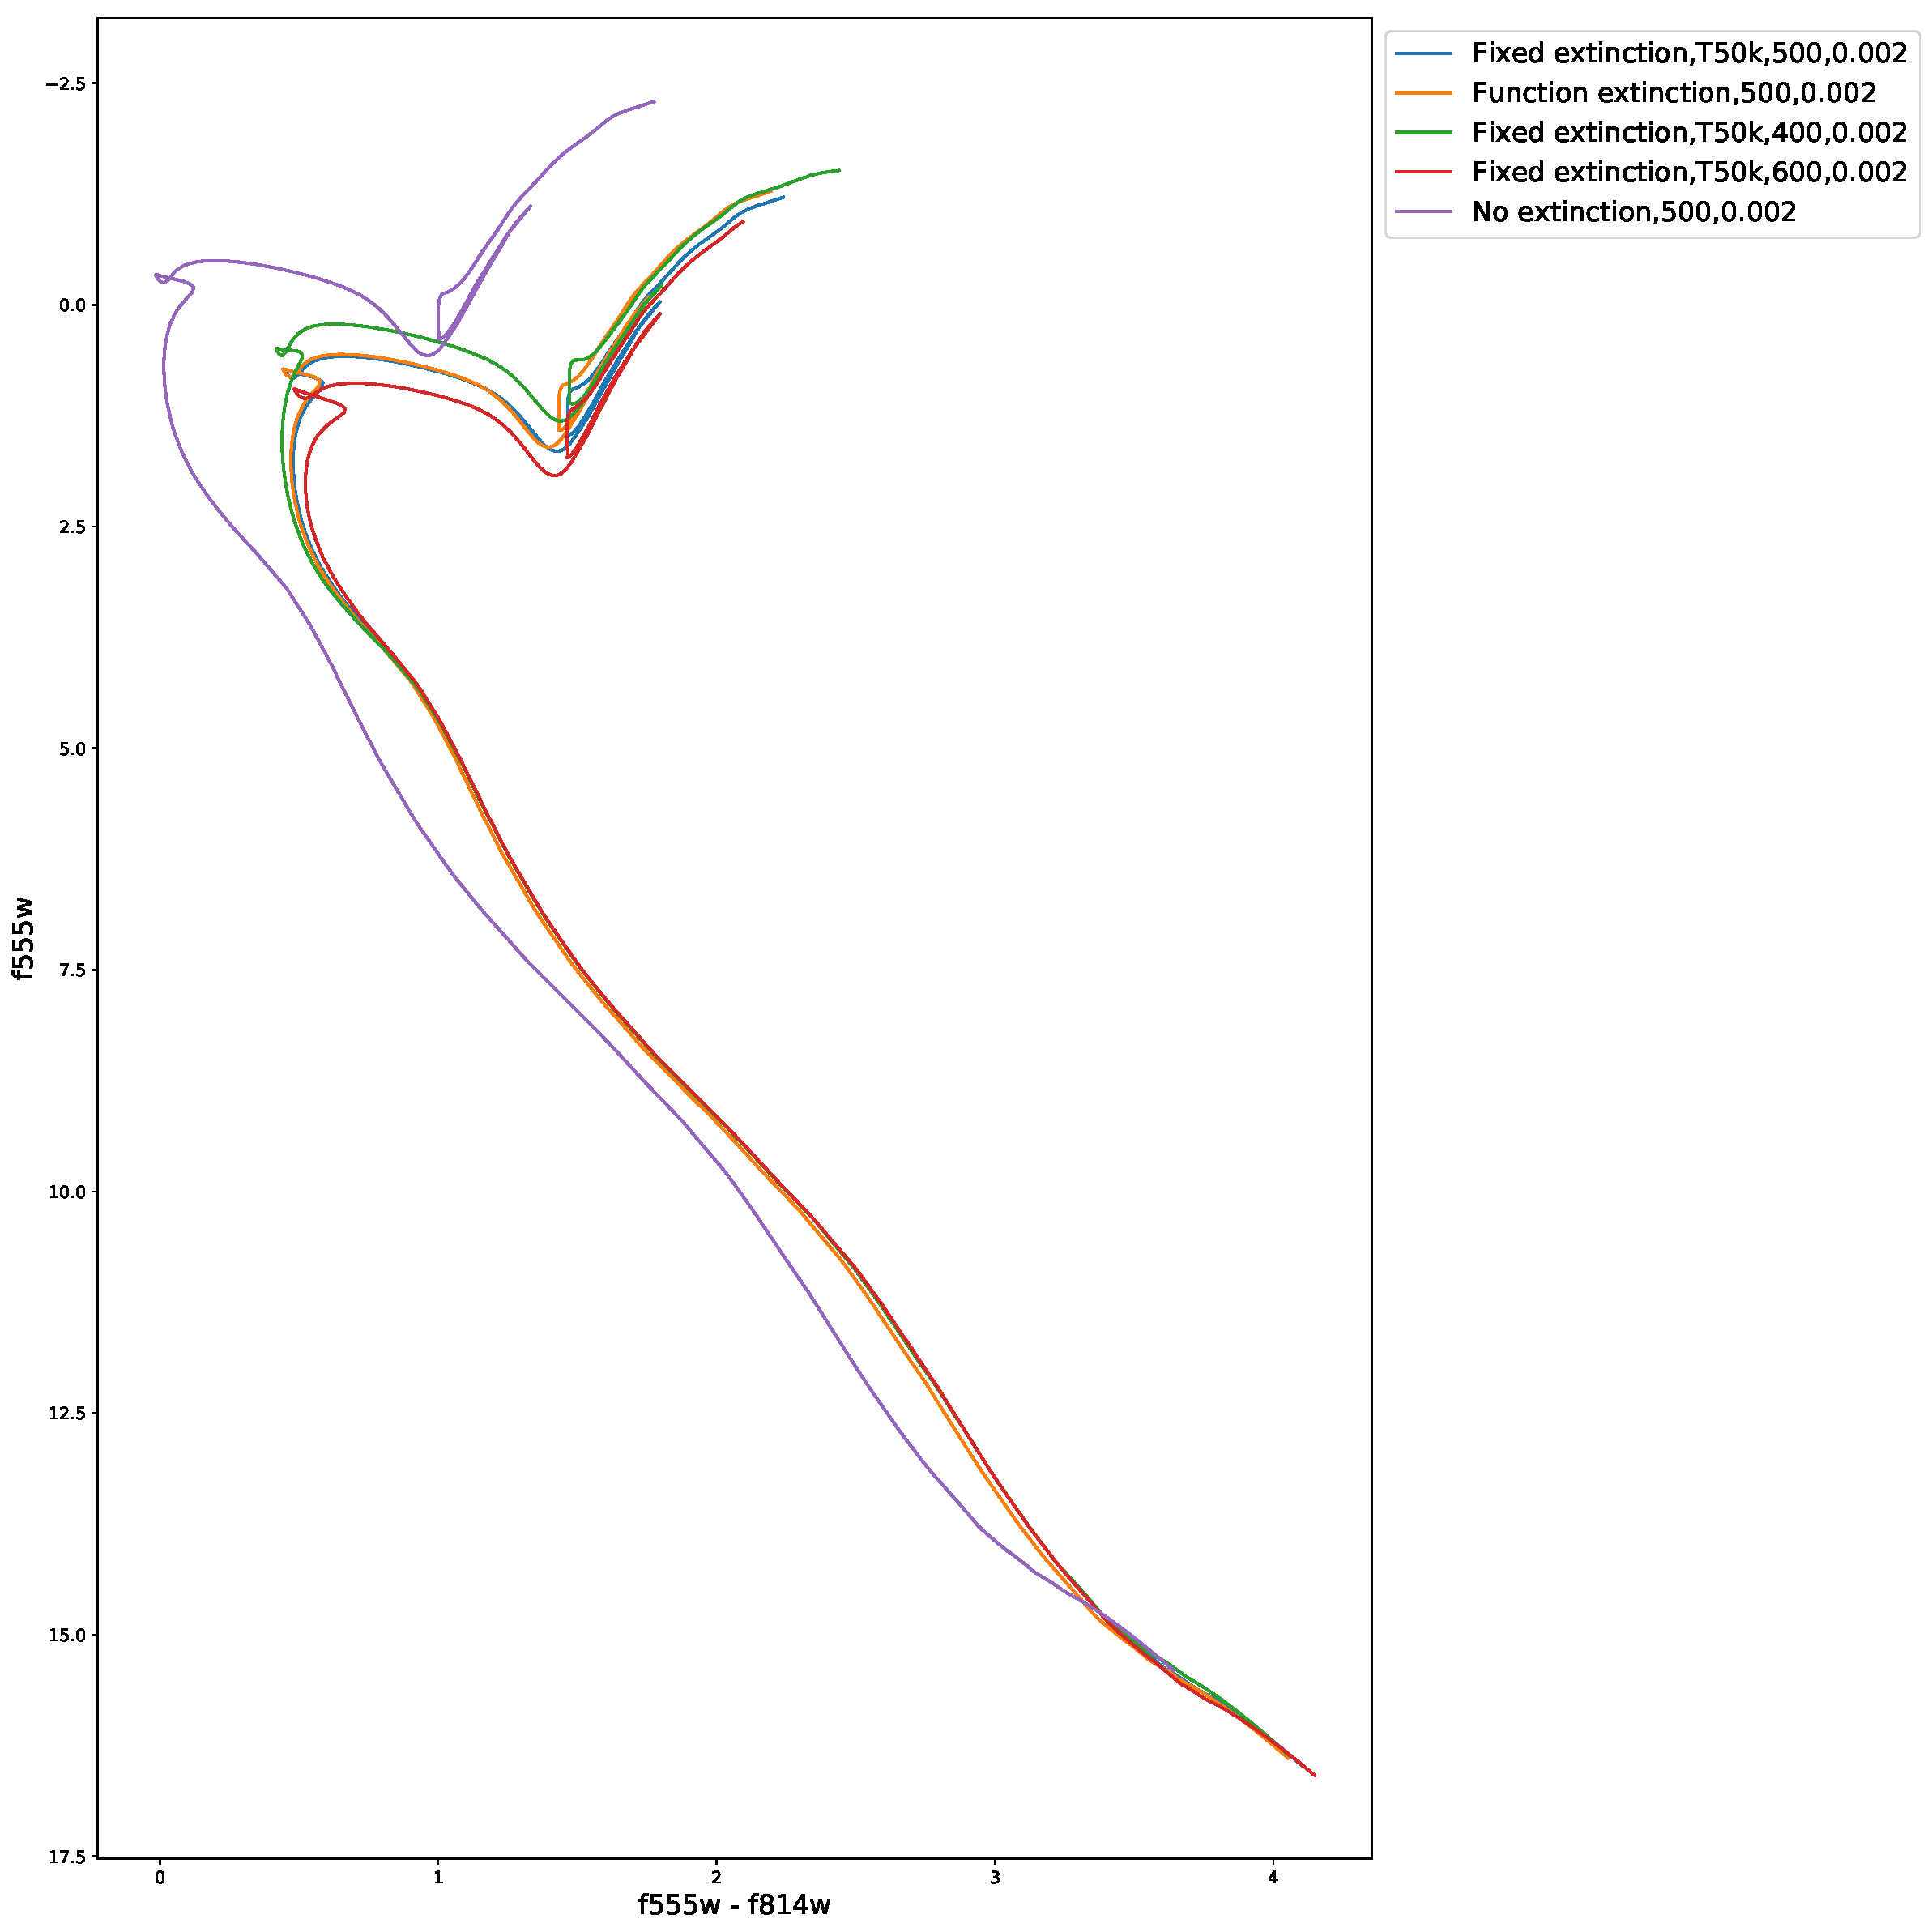
\includegraphics[width=1.0\textwidth]{../basti_isochrones_10_13Gyr/Extinction_T50k_FeH0fix_func_f555w_f555wmf814w_500_400_600_Myr_FeH_0p002_ref_noext_Av_1p0.pdf}
\caption{WFC3 F555W-(F555W-F814W) CMD with a fixed extinction value equal to $(A_{X}/A_{V})_{plat}$ for each filter}
\label{wfc3_isoc1_T50k}
\end{center}
\end{figure}

The second WFC3 CMD that was studied is the F814W-(F275W-F814W) CMD. The filters that form this CMD cover the soft-UV and near-IR spectral regions. The high baseline wavelength coverage of this combination of filters makes the colour index more sensitive to differences in $T_{\textnormal{eff}}$ in hot horizontal branch (HB) stars. These objects are important due to direct helium abundance measurements (from absorption lines) being available in globular clusters only for HB stars with 8000 $\lesssim T_{\textnormal{eff}}$ / K $\lesssim$ 11500 \citep{2018MNRAS.475.4088L}.

\begin{figure}[h]
\begin{center}
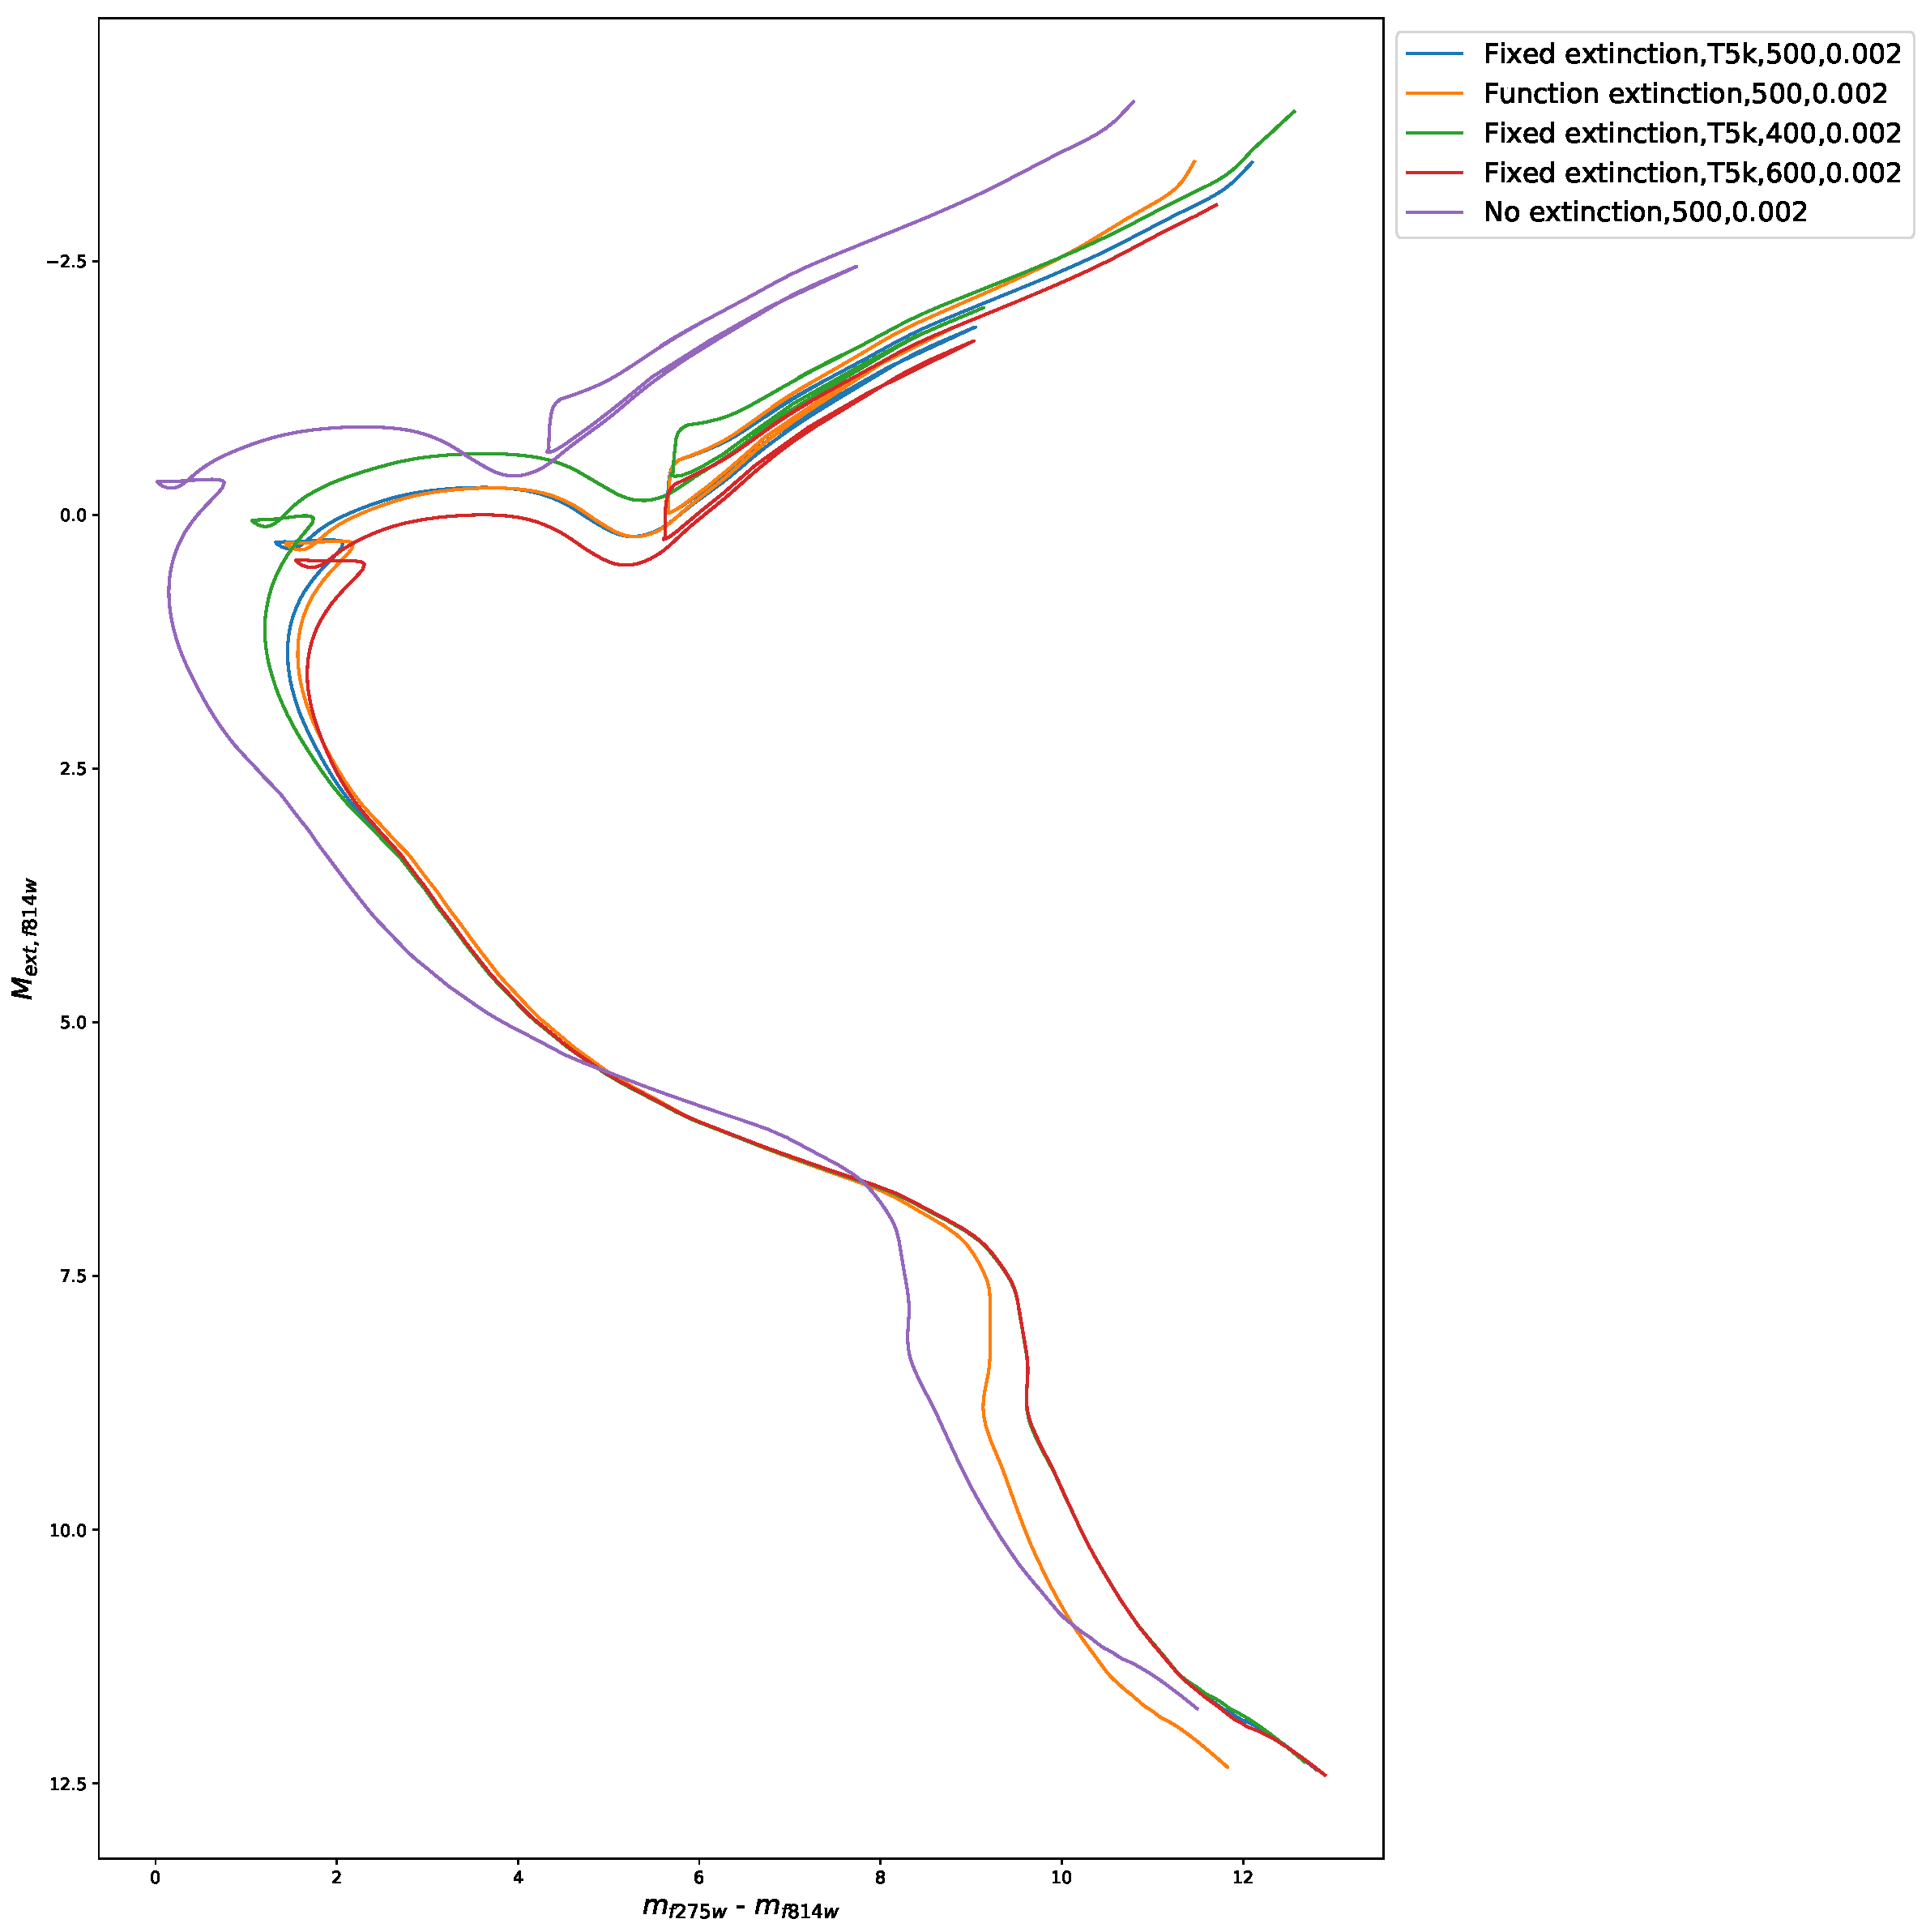
\includegraphics[width=1.0\textwidth]{../basti_isochrones_10_13Gyr/Extinction_T5k_FeH0fix_func_f814w_f275wmf814w_500_400_600_Myr_FeH_0p002_ref_noext_Av_1p0.pdf}
\caption{WFC3 F814W-(F275W-F814W) CMD with a fixed extinction value equal to $(A_{X}/A_{V})_{MS}$ for each filter.}
\label{wfc3_isoc2_T5k}
\end{center}
\end{figure}

\begin{figure}[h]
\begin{center}
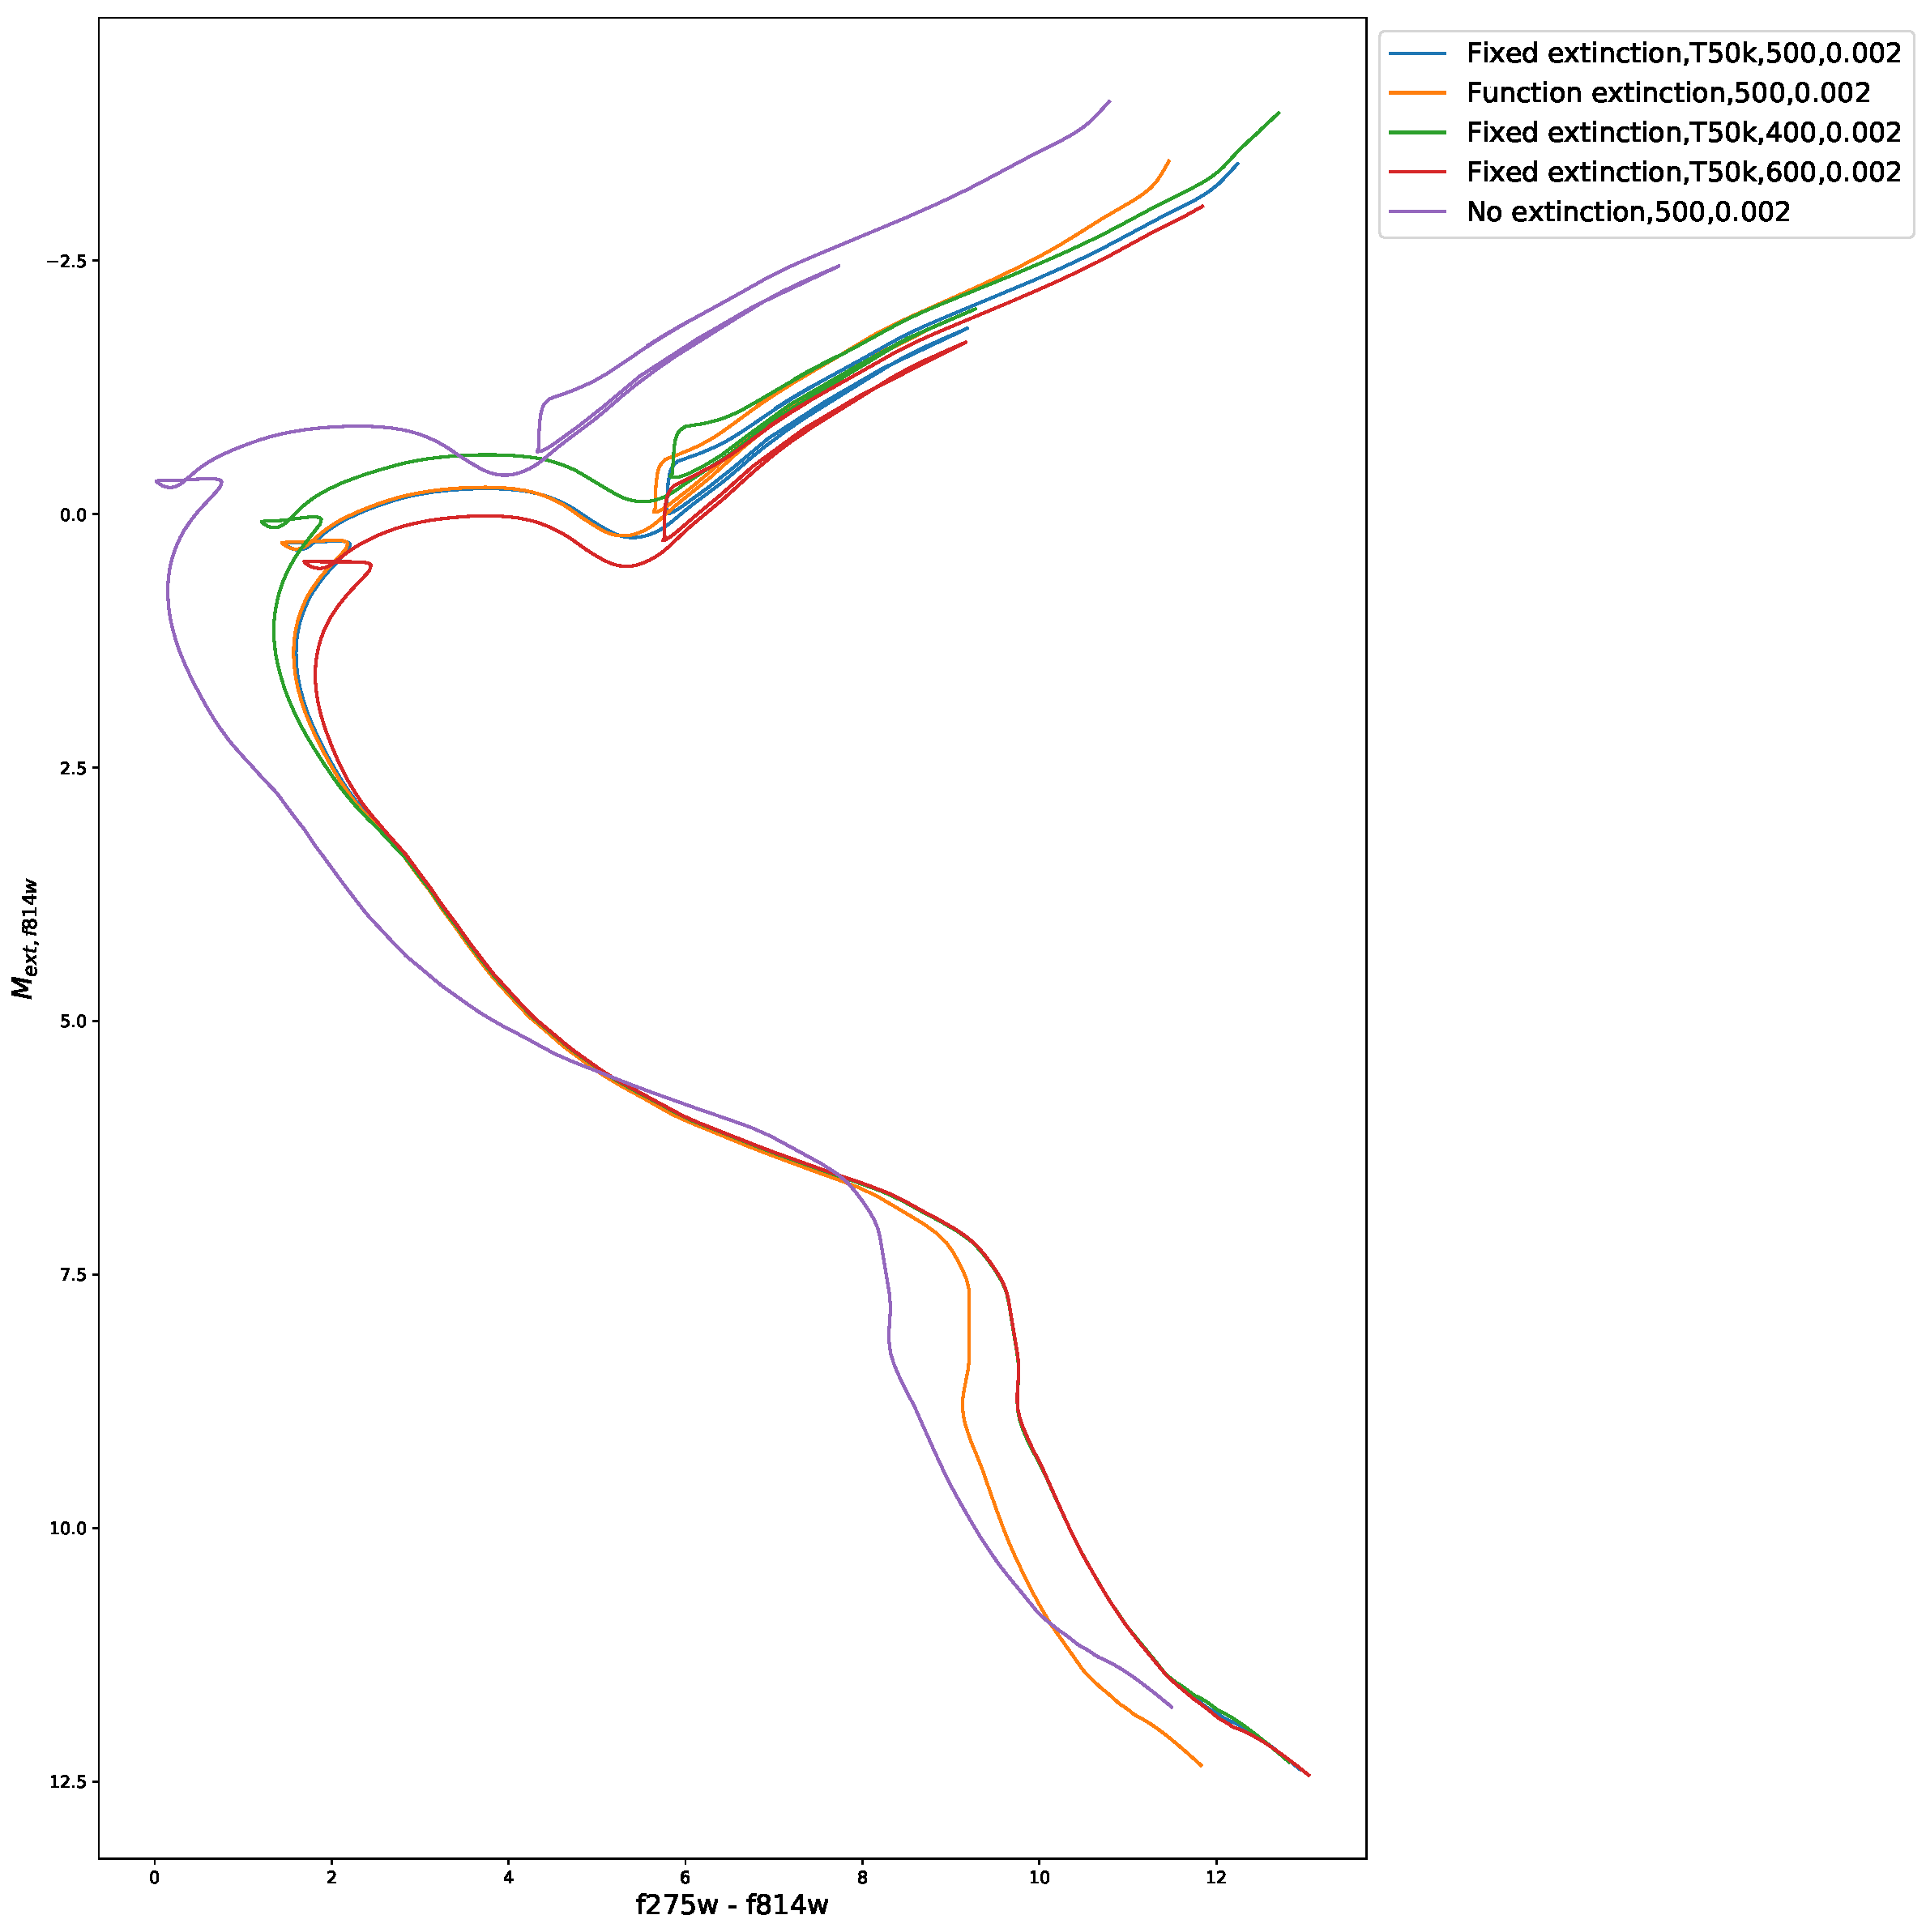
\includegraphics[width=1.0\textwidth]{../basti_isochrones_10_13Gyr/Extinction_T50k_FeH0fix_func_f814w_f275wmf814w_500_400_600_Myr_FeH_0p002_ref_noext_Av_1p0.pdf}
\caption{WFC3 F814W-(F275W-F814W) CMD with a fixed extinction value equal to $(A_{X}/A_{V})_{plat}$ for each filter}
\label{wfc3_isoc2_T50k}
\end{center}
\end{figure}

In Figure \ref{wfc3_isoc2_T5k}, it can be seen that, when $(A_{X}/A_{V})_{MS}$ fixed model is being used as a reference (i.e., the models' upper main sequences below the MSTO are aligned), the position of the MSTO of the FBER 500 Myr isochrone aligns with that of the 600 Myr fixed-ratio isochrone. By the point at which the MS hook \citep{1998MNRAS.298..525P} appears, the FBER isochrone has almost realigned with the 500 Myr fixed-ratio isochrone. There are significant differences between the two 500 Myr isochrones after the lower portion of the RGB. In the lower main sequence, all isochrones with fixed extinction ratios appear significantly redder, while the infrared F814W magnitudes appear to be more or less unchanged from the FBER case. This can only be the result of significant differences in $A_{F275W}/A_{V}$ values between models in the upper main sequence (higher $T_{\textnormal{eff}}$ values) and in the lower main sequence (lower $T_{\textnormal{eff}}$ values), as these differences are not reflected in the fixed-extinction models. \\*

In Figure \ref{wfc3_isoc2_T50k}, choosing $(A_{X}/A_{V})_{plat}$ for the fixed-extinction isochrones leads to those isochrones shifting down and to the right. Ironically, the higher $T_{\textnormal{eff}}$ value of 50,000 K used, which is far greater than any $T_{\textnormal{eff}}$ values present in the isochrone data, brings the MSTO positions of the two 500 Myr isochrones back into alignment. However, the use of $(A_{X}/A_{V})_{plat}$ increases the lower main sequence gap between the fixed-extinction and FBER isochrones. Beyond the lower main sequence, the misalignment between the 500 Myr isochrones now begins at a later stage in the evolutionary cycle, at the base of the RGB. \\*

Furthermore, there is a possibility of the extinction-related lower main sequence discrepancy causing a further discrepancy in the estimated metallicity when an isochrone is fitted to the observed CMD of a cluster, as the CMD position of this part of the isochrone is the most sensitive to changes in isochrone metallicity.\\*

\subsection{Gaia} \label{Gaia_isoc}

The photometric filters in Gaia, as shown by their respective response functions in Figure \ref{Gaia_response_funcs}, are designed such that the only useful colour index is the ($G_{\textnormal{bp}}-G_{\textnormal{rp}}$) index, with the widest filter ($G$) being on the vertical axis.\\*

\begin{figure}[h]
\begin{center}
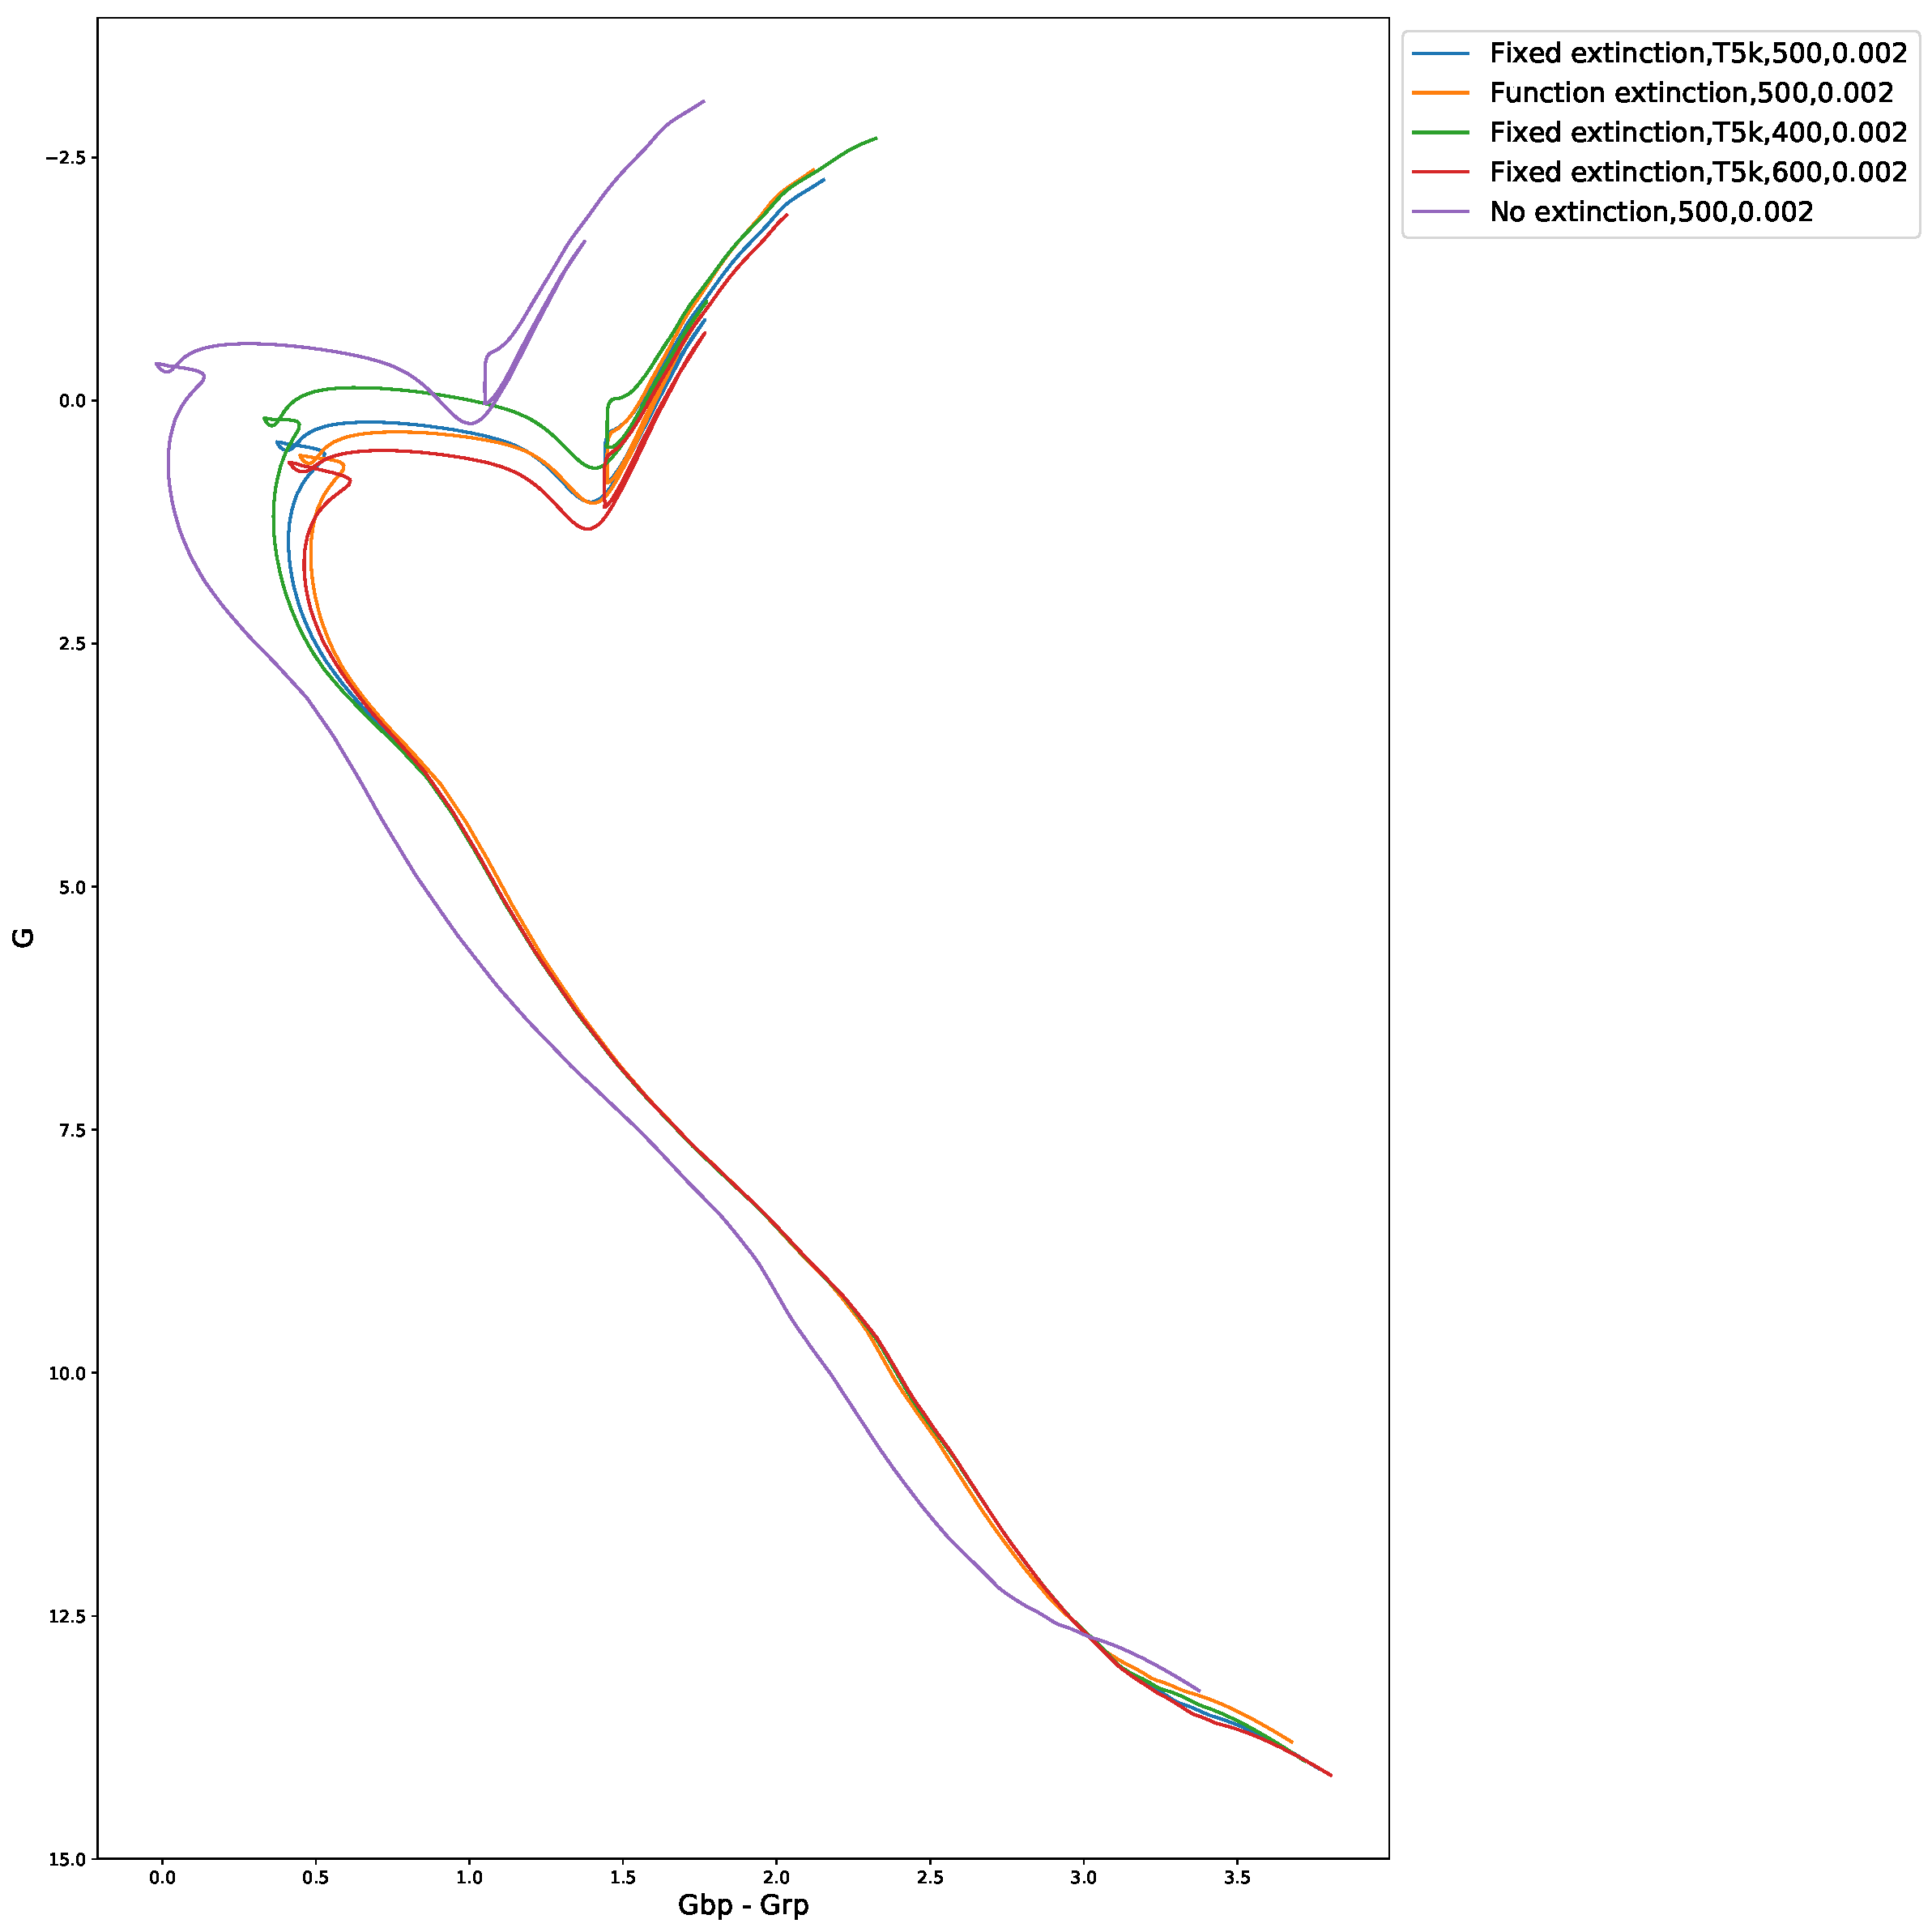
\includegraphics[width=1.0\textwidth]{../basti_isochrones_10_13Gyr/Extinction_T5k_FeH0fix_func_G_GbpmGrp_500_400_600_Myr_FeH_0p002_ref_noext_Av_1p0.pdf}
\caption{Gaia $G$-($G_{\textnormal{bp}}$-$G_{\textnormal{rp}}$) CMD with a fixed extinction value equal to $(A_{X}/A_{V})_{MS}$ for each filter}
\label{gaia_isoc_T5k}
\end{center}
\end{figure}

\begin{figure}[h]
\begin{center}
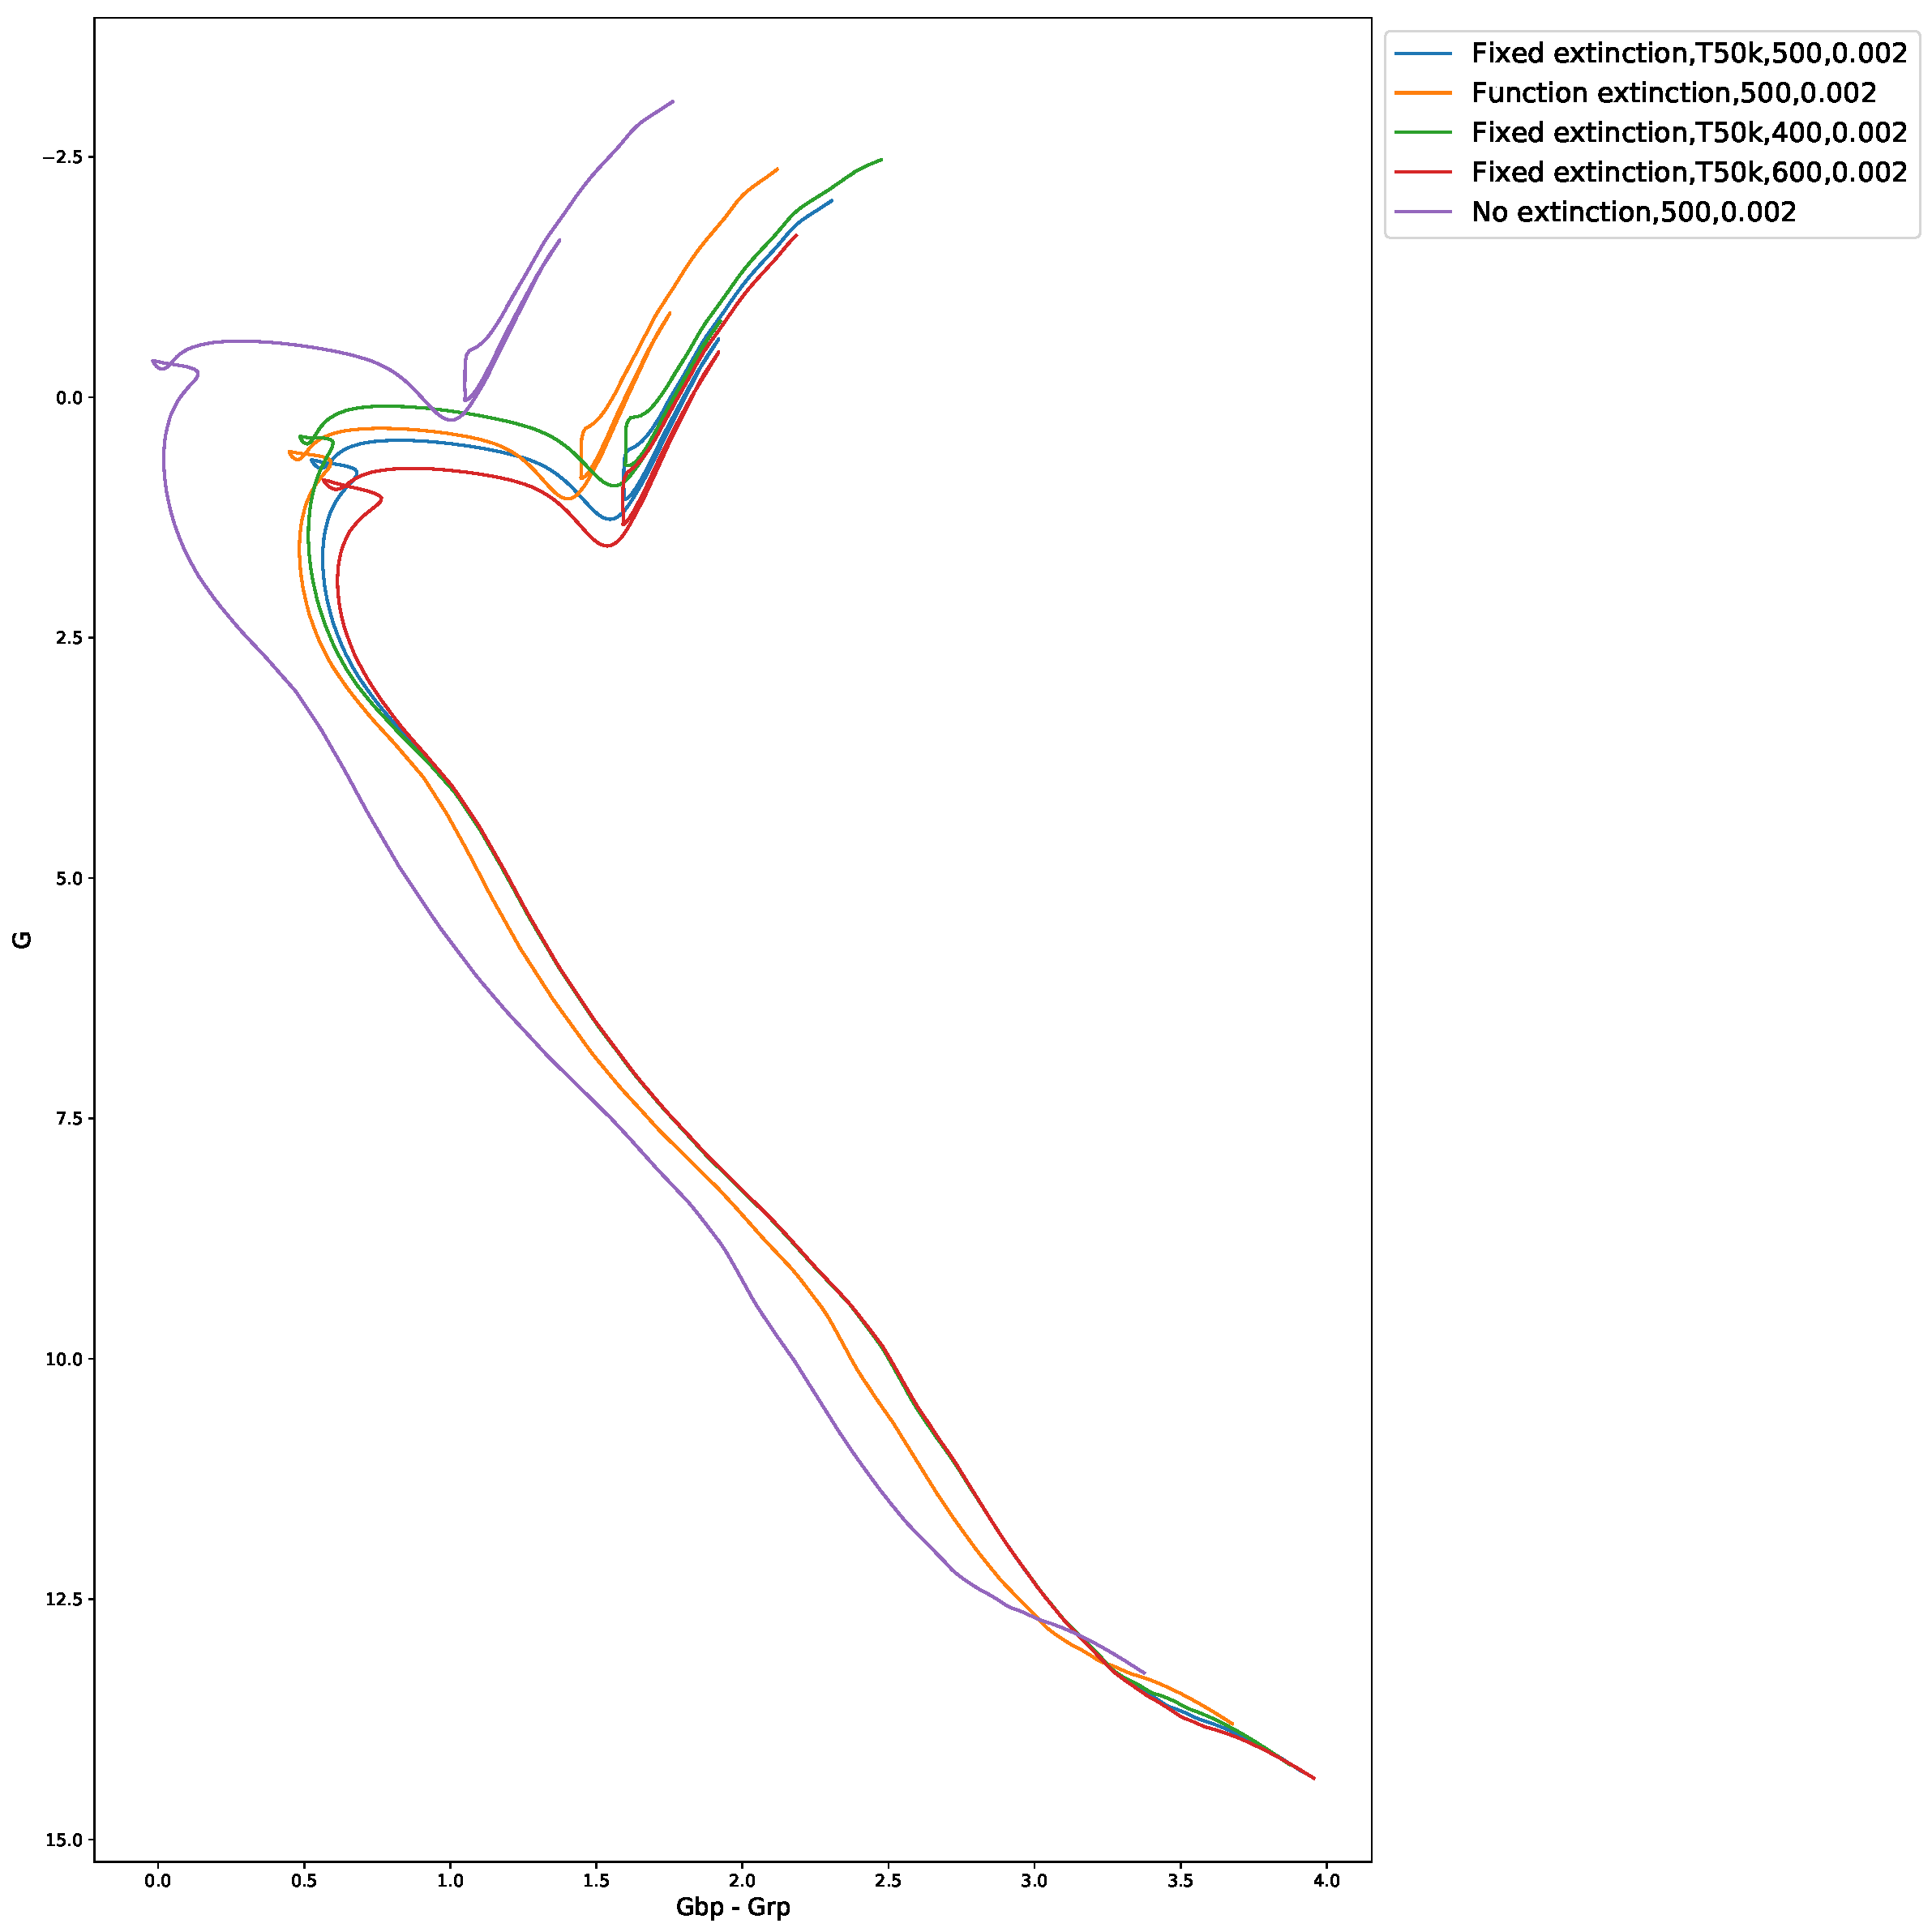
\includegraphics[width=1.0\textwidth]{../basti_isochrones_10_13Gyr/Extinction_T50k_FeH0fix_func_G_GbpmGrp_500_400_600_Myr_FeH_0p002_ref_noext_Av_1p0.pdf}
\caption{Gaia $G$-($G_{\textnormal{bp}}$-$G_{\textnormal{rp}}$) CMD with a fixed extinction value equal to $(A_{X}/A_{V})_{plat}$ for each filter}
\label{gaia_isoc_T50k}
\end{center}
\end{figure}

For the Gaia CMD, when $(A_{X}/A_{V})_{MS}$ is used for the fixed-extinction ratio isochrones, as shown in Figure \ref{gaia_isoc_T5k}, the turnoff position of the 500 Myr FBER isochrone appears to be lower on the main sequence than even the 600 Myr fixed-extinction case, suggesting that using the fixed-extinction treatment significantly and consistently over-estimates the isochrone age for an observed cluster. However, unlike the F814W-(F275W-F814W) CMD, the alignment of the main sequence continues almost along the  entire MS length. \\*

When using $(A_{X}/A_{V})_{plat}$ for the fixed-extinction isochrone, the whole isochrone is shifted down and to the right when moving from the FBER isochrone to the fixed-extinction isochrone, as can be seen in Figure \ref{gaia_isoc_T50k}. Since all four isochrones with added extinction in this figure assume that $A_{V} = 1.0$, alignment of the upper main sequences when using $(A_{X}/A_{V})_{plat}$ can only be achieved by having a lower value of $A_{V}$ for the fixed-extinction isochrones than for the function-based case. Depending on the exact value of the fixed $A_{X}/A_{V}$ used for fitting an isochrone to a given observed cluster, the resulting value calculated for $A_{V}$ and, subsequently, $E(B-V)$ could be significantly underestimated. \\*


\section{NGC 6793}
\subsection{Uncertainties in observational data}

\begin{figure}[h!]
\begin{center}
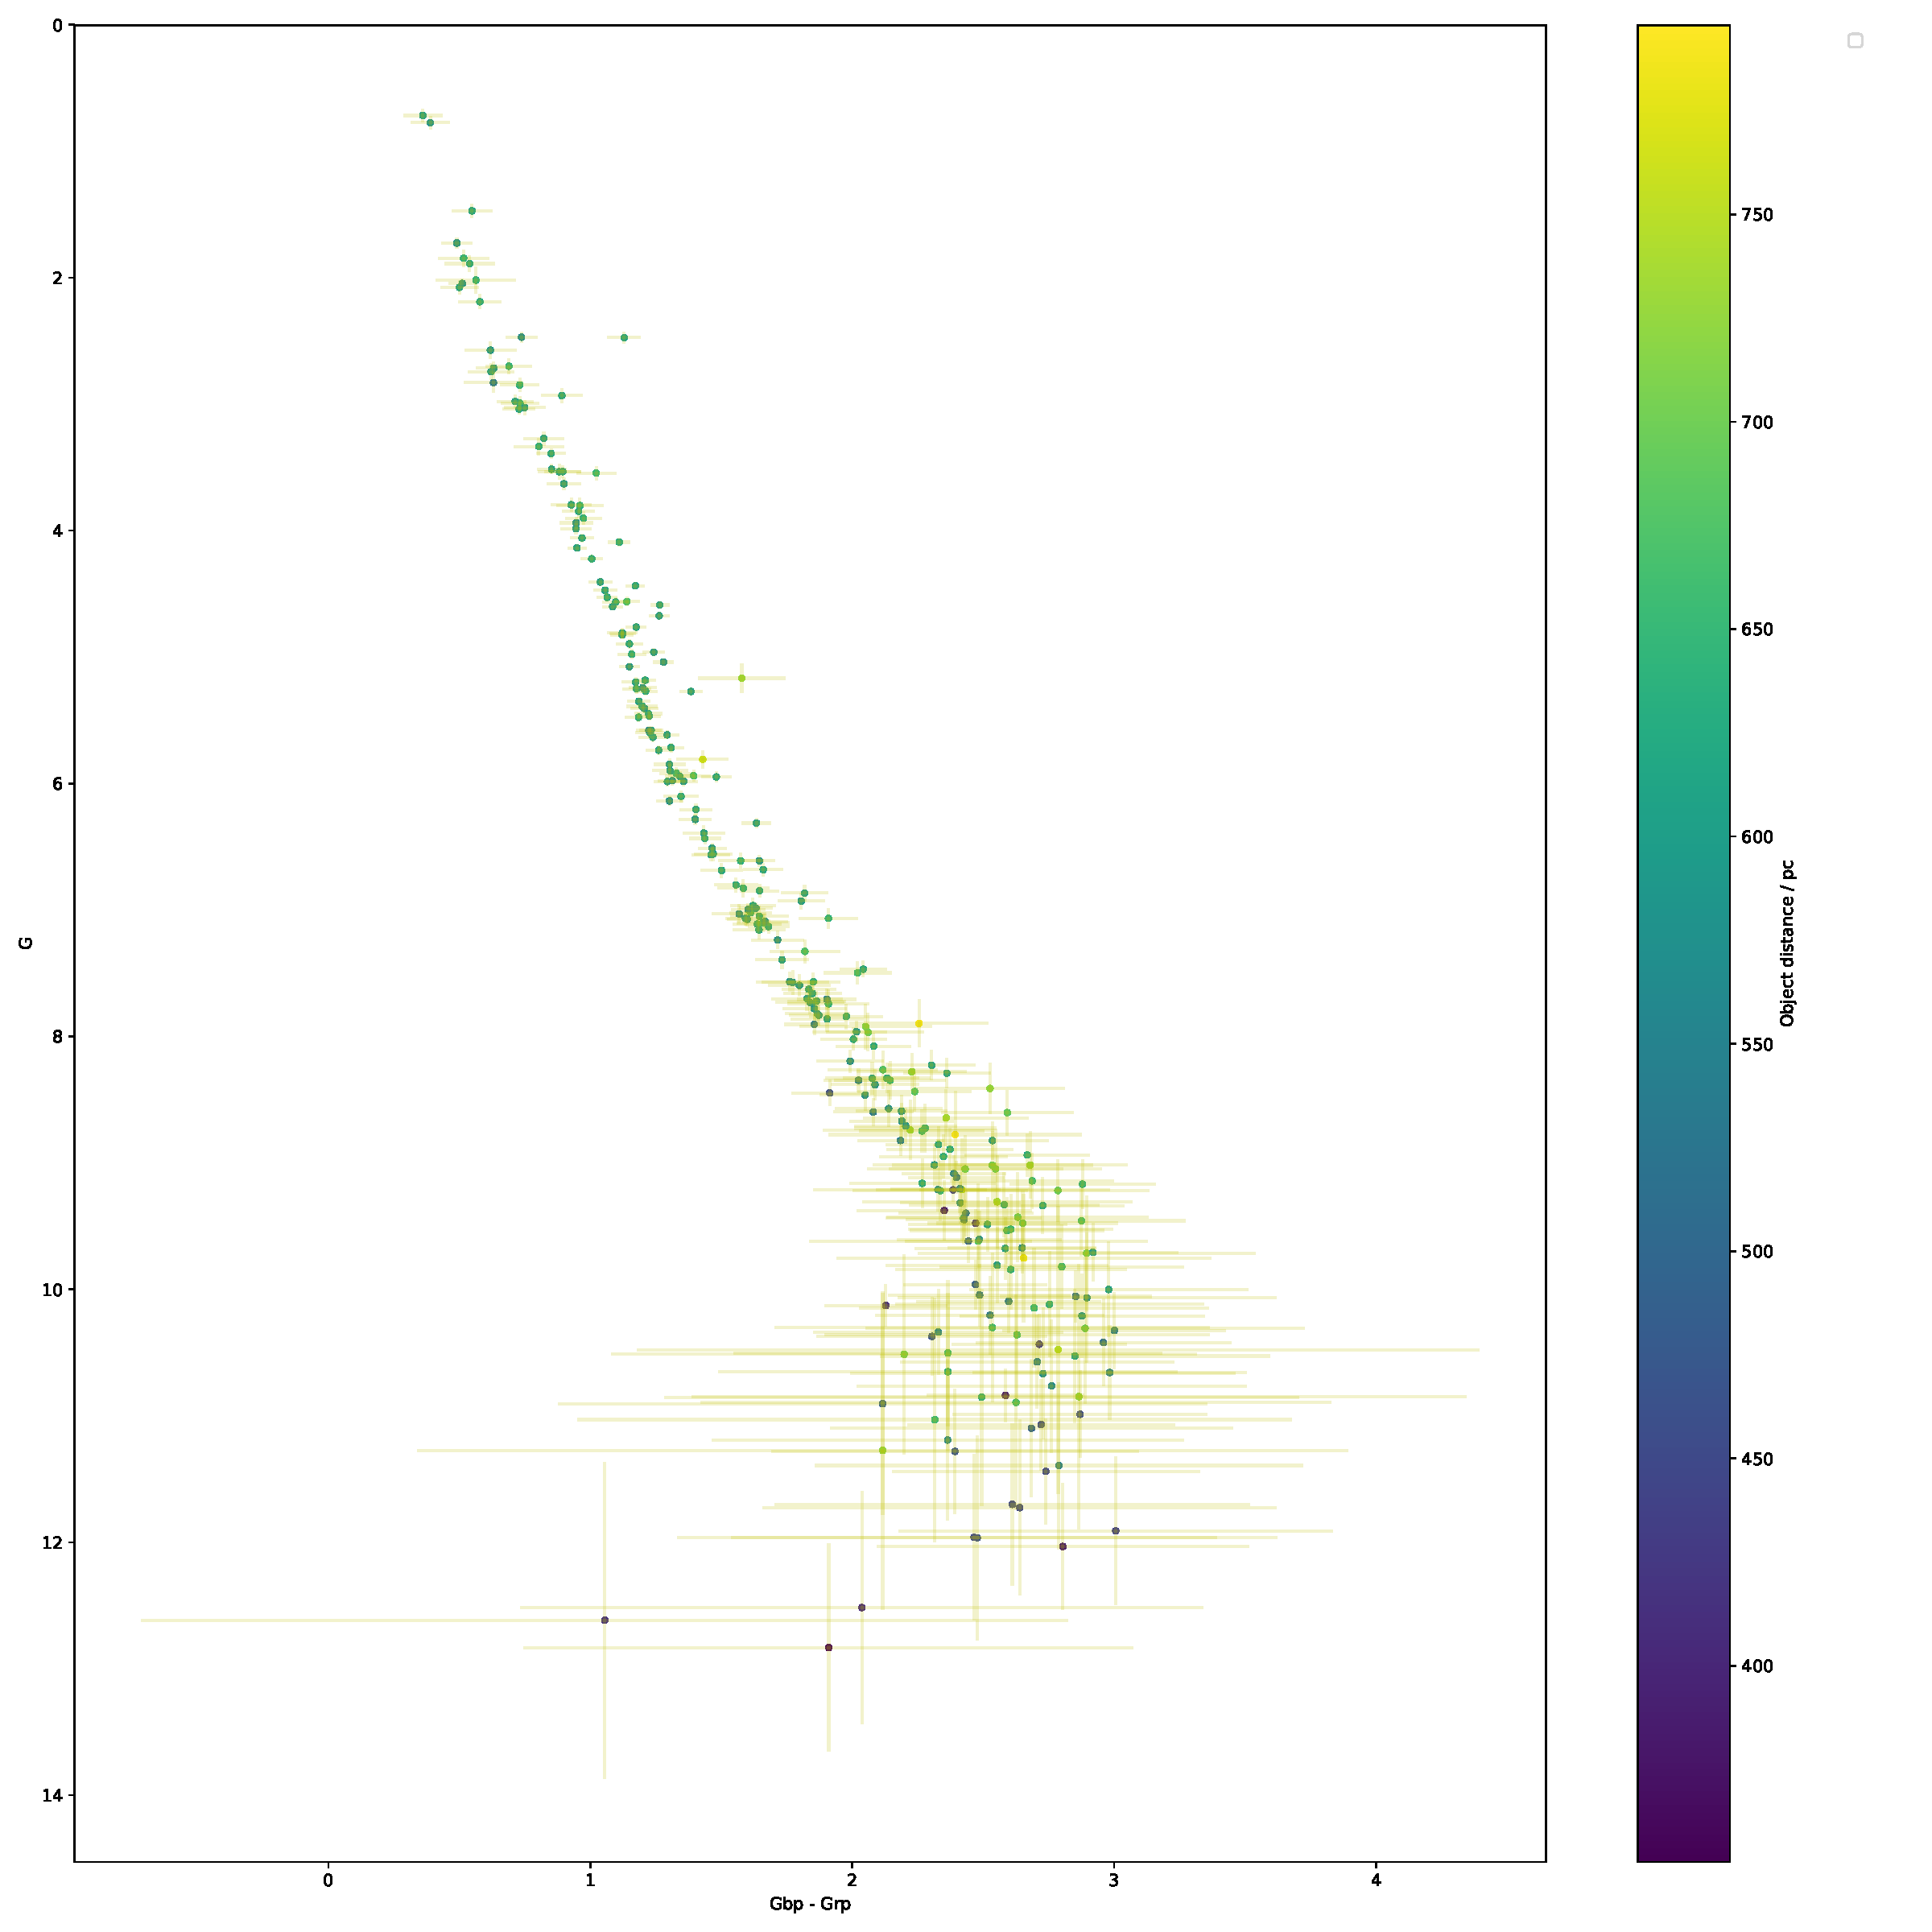
\includegraphics[width=1.0\textwidth]{../NGC_6793_CMD_observational_errorbars.pdf}
\caption{Gaia $G$-($G_{\textnormal{bp}}$-$G_{\textnormal{rp}}$) CMD of NGC 6793, showing the 274 cluster members in the final dataset, corrected for their individual distances with errorbars shown. The color of each object is determined by its parallax-derived distance.}
\label{NGC_6793_obs_only}
\end{center}
\end{figure}

\begin{figure}[h]
\begin{center}
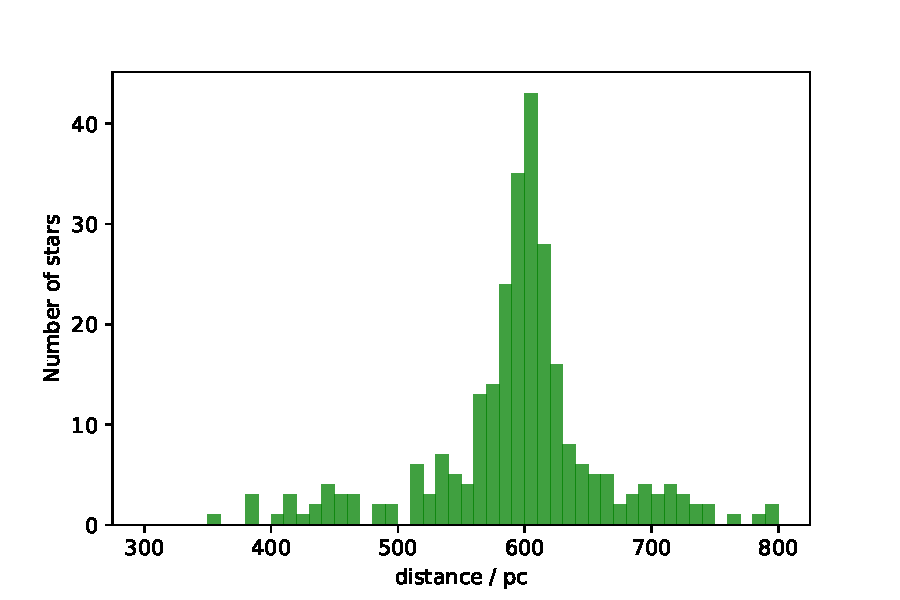
\includegraphics[width=1.0\textwidth]{../NGC_6793_distances_hist.pdf}
\caption{Histogram of distances for the 274 stars in the final observational dataset. The bins are set to a fixed width of 10 pc.}
\label{NGC_6793_dist_hist}
\end{center}
\end{figure}

The final Gaia observational sample of stars in NGC 6793 is shown as a distance-corrected CMD in Figure \ref{NGC_6793_obs_only}, with distances and photometric errors propagated directly from parallax measurements.\\*

However, the uncertainties in the parallax data for objects assigned to NGC 6793 were significant, as shown in Figure \ref{NGC_6793_obs_only}, for stars in the lower main sequence. This is trend is to be expected, since stars in the lower main sequence are the faintest objects in the data and therefore are the most difficult to track against background sources. The significance of the uncertainties persists despite this project assuming that the only sources of photometric error are the parallax measurements. This leads to uncertainties in the predicted $M_{\textnormal{ext},X}$ magnitudes, which are calculated by rearranging Equation \ref{ext_def_app_mag}.\\*

Since the table of photometric magnitudes did not include photometric errors, the parallax errors alone accounted for the total error in the calculated $M_{\textnormal{ext},X}$ values. Therefore, the propagated errors for the $M_{\textnormal{ext},X}$ values were fully independent of the value of the absolute magnitude of a given star. The parallax-derived errors on the ($G_{\textnormal{bp}}-G_{\textnormal{rp}}$) colour index are zero, as an object's colour index can simply be calculated as the difference between its apparent magnitudes in both filters, and is therefore independent of the object's parallax.\\*

Looking at the distances to the objects in the final sample shown in Figure \ref{NGC_6793_dist_hist}, it is clear that there are significant variations in the observed parallaxes of individual stars, far beyond the maximum cluster radii expected for the largest open clusters, given as 16.8$\pm$2.4 pc by \cite{2006A&A...456..523S} or even radii of compact stellar associations, given as 33.2$\pm$21.7 pc in the same paper. Some objects in the original dataset (which contains 338 members in total) were even assigned negative parallax values, which are physically impossible, as a result of measurement errors. Figure \ref{NGC_6793_dist_hist} shows a histogram of stars in the final NGC 6793 sample, binned by the parallax-derived distance. It is clear that a substantial fraction of this sample have measured parallax distances which put them outside the physical limits determined from other, better-studied open clusters, even after the distance limits outlined in Section \ref{obs_ngc_section} were imposed. On the other hand, applying stricter distance limits, in line with those given by \cite{2006A&A...456..523S}, produced a dataset with too few stars remaining for . This led to the decision to impose limits resulting in a dataset of similar size to that used by GC18. In summary, therefore, there are additional uncertainties from the data due to selection of questionable sources as cluster members. \\*

\subsection{Isochrones}

\begin{figure}[h]
\begin{center}
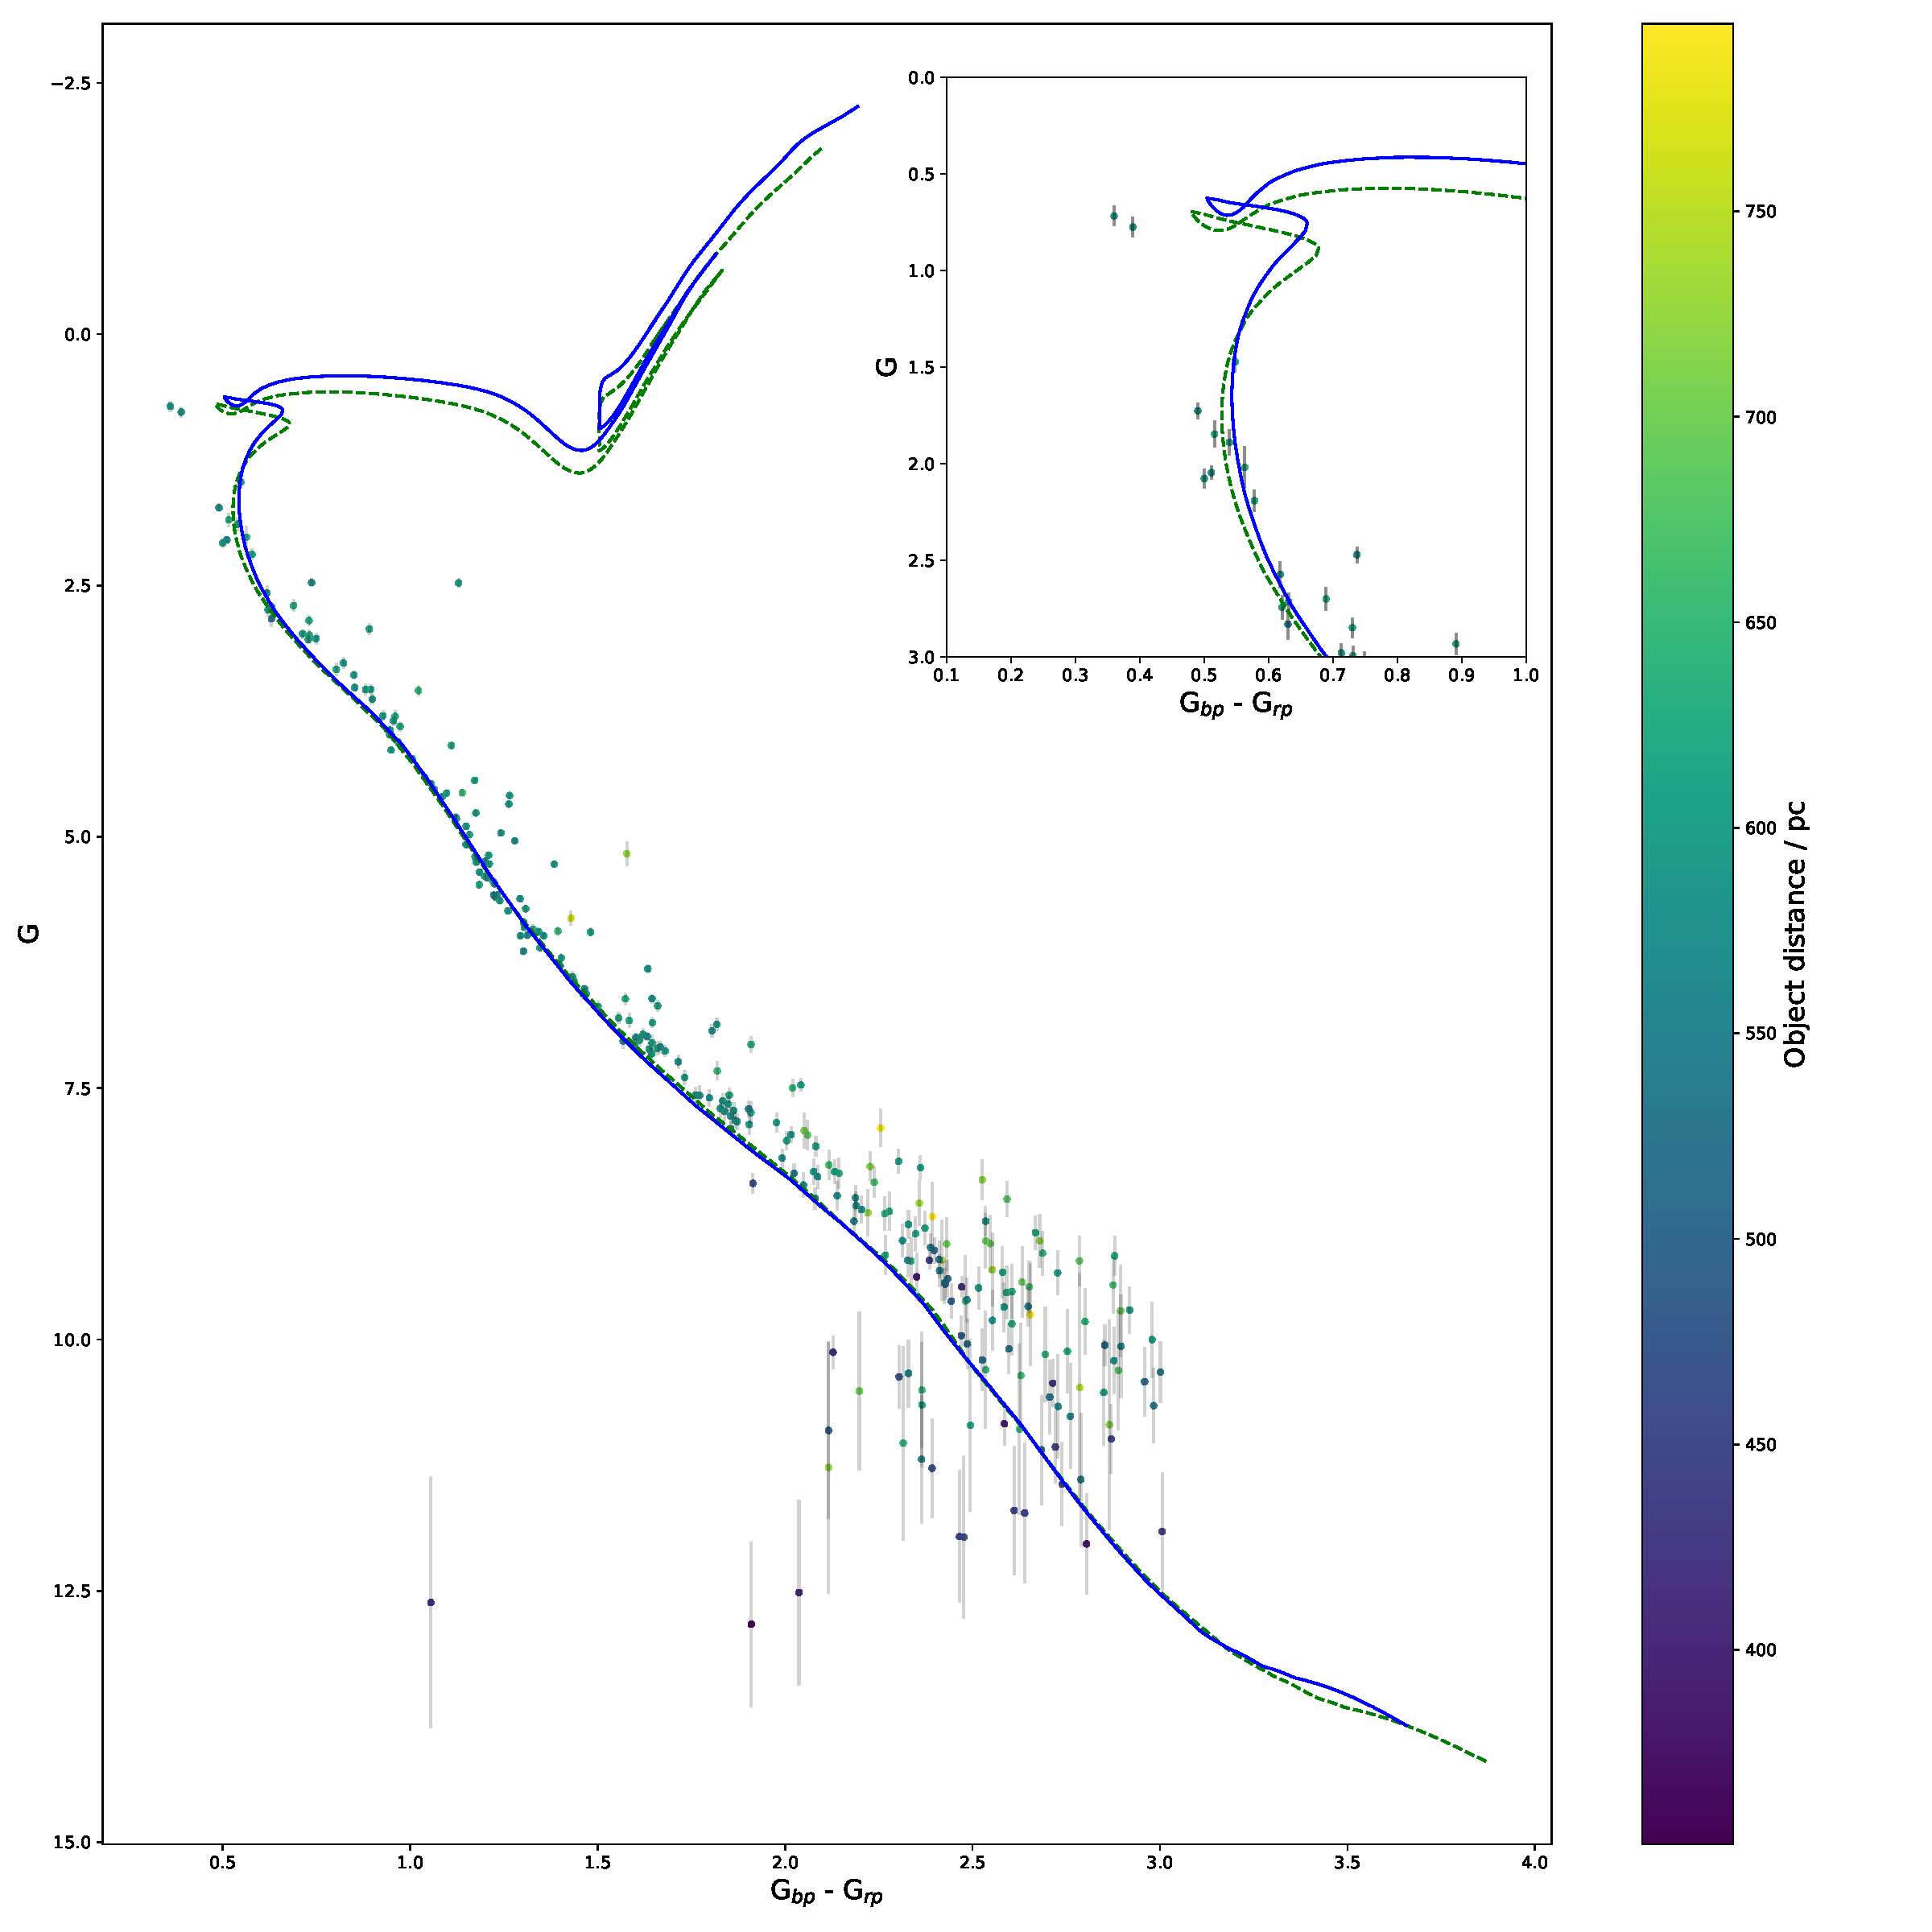
\includegraphics[width=1.0\textwidth]{../NGC_6793_CMD_FeH_0p062_Av_1p1_500Myr_all_xloge_correction_no_xerr_isochrones_summary_errorbars.pdf}
\caption{Gaia $G$-($G_{\textnormal{bp}}$-$G_{\textnormal{rp}}$) CMD of NGC 6793, showing the 274 distance-corrected cluster members in the final dataset overlaid with a isochrone treated with a fixed extinction-ratio value of $(A_{X}/A_{V})_{plat}$ and age, $A_{V}$ and [Fe/H] values taken from the GC18 results in Table \ref{NGC6793_obs} and a 500-Myr FBER isochrone (solid blue) with an $A_{V}$ value of 1.1 and a metallicity of [Fe/H] = 0.062, with the parallax-derived errorbars added. The inset panel shows a zoomed-in view of the MSTO region.}
\label{NGC_6793_isoc_inset_1.1_500_0.062}
\end{center}
\end{figure}

Before comparisons between the GC18 results and those for a FBER-based fit can be made, a reference isochrone, with a globally-fixed $A_{V}$ value of 0.843 and age of 600 Myr (in accordance with the GC18 values in Table \ref{NGC6793_obs}), was created. This was done to test whether or not the GC18 resultsThe $A_{X}/A_{V}$ values required for this isochrone to achieve alignment with the upper main sequence below the MSTO were equal to the $(A_{X}/A_{V})_{plat}$ values for each Gaia filter. While the results from GC18 do not include a metallicity estimate for NGC 6793, it can be estimated from its age that a solar-like metallicity is likely. Therefore, the relevant isochrone has a metallicity of [Fe/H] = 0. Due to the overall red-ward shift of an isochrone when treated with an extinction ratio of $(A_{X}/A_{V})_{plat}$, rather than the physically more-realistic $(A_{X}/A_{V})_{MS}$, as demonstrated in Figure \ref{gaia_isoc_T50k}, the GC18 parameter values, in particular the listed $A_{V}$ value of 0.843, do not produce an accurate fit when using the FBER treatment in the isochrones for the NGC 6793 observational data.\\*

Before making an age estimate, the main sequence of the FBER isochrone had to align with the MS of NGC 6793. It was found that the positions of MS objects in the region $1.0 \lesssim (G_{\textnormal{bp}}-G_{\textnormal{rp}}) \lesssim 1.5$, well below the MSTO, varied the least with changes in metallicity for the FBER isochrone. By contrast, changing the $A_{V}$ value applied to the isochrone produced a more homogeneous shift in positions along the entire isochrone, as would be expected. Therefore, the initial alignment of this region was achieved by placing greater importance on the isochrone $A_{V}$ value than on the metallicity. The metallicity variations were then used to align the remaining regions of the MS with the observed data. Finally, isochrones of different ages were plotted to determine the best-fit cluster age. \\*

The alignment of this MS region for a FBER treatment was achieved using a value of $A_{V} = 1.1$. To better align the FBER isochrones to the lower main sequence, an increase in isochrone metallicity was required. The best-fit metallicity value was found to be [Fe/H] = 0.062. However, the magnitudes of the observational errorbars in $M_{\textnormal{ext},G}$ for lower MS stars (see Figure \ref{NGC_6793_obs_only}) dwarf any isochrone position changes due to changing extinction treatments in the main sequence. Once these parameters were determined, the isochrone with best-fitting MSTO position had an age of 500 Myr. In addition, there are significant uncertainties due to a lack of errors for the photometric measurements. Having such errors included would not only increase the $M_{\textnormal{ext},G}$ errorbar sizes, but also add in another set of errorbars for the colour axis, increasing the overall uncertainties in the best-fit values of the isochrone parameters. \\*


\begin{table}
\begin{center}
\begin{tabular}{ccccc}
\hline
Cluster property & K05 & K13 & GC18 & This project \\
\hline
Age / Myr & 437 & 495 & 603 & 500 \\
$A_{V}$ / mag & 0.53 & 0.967 & 0.843 & 1.1 \\
$\textnormal{[Fe/H]}$ & ? & ? & ? & 0.062 \\
Members & ? & 133 & 271 (photometric) & 274 \\
\hline
\end{tabular}
\caption{Comparison of results from this project with results of previous studies of NGC 6793.}
\label{NGC6793_result}
\end{center}
\end{table}

The wide range of distances determined for the individual stars included in the final sample, as mentioned earlier, is orders of magnitude greater than is the case for the largest better-known clusters. Stars whose distances place them furthest from the projected cluster centre make up a significant portion of the objects which are widely scattered from the expected position of the main sequence. Therefore, between this and the magnitude of the errorbars in the lower main sequence in particular, the isochrone fits shown in Figure \ref{NGC_6793_isoc_inset_1.1_500_0.062} can be considered accurate. \\*

A potential source of uncertainty when comparing the best-fit isochrone results of this project for NGC 6793 with those from GC18 comes from the fact that this project employs the latest BaSTI isochrone database \citep{2018ApJ...856..125H}, while GC18 uses the PARSEC isochrone database \citep{2017ApJ...835...77M}. This project's use of ischrones generated by a different model stellar evolution code from that used by GC18 for their isochrones could impact the validity of comparing the $A_{V}$ values, ages and metallicities arising from both extinction treatments.\\*

A recent comparison of isochrones, including those generated using BaSTI and PARSEC, was made by \cite{2019MNRAS.483.4949G}. The authors carried out a detailed set of observations of the Galactic globular cluster NGC 5904 in 29 photometric bands. The CMDs created from this data were used to fit isochrones from five different databases, including PARSEC and BaSTI. They adopted the \cite{1989ApJ...345..245C} extinction law with the parameters having values of $R_{V} = 3.60\pm0.05$ and $A_{V} = 0.20\pm0.02$. As shown in Table \ref{NGC5904_obs_gontcharov}, the Gaia colour excess $E(G_{\textnormal{bp}} - G_{\textnormal{rp}})$ for NGC 5904 differs significantly between the best-fits from the two databases, which in turn causes disagreements for the projected cluster age and (photometric) distance. Across all filter systems and isochrone databases, the authors calculated mean estimates of the cluster properties and found that the resulting photometric distance to be in agreement with the cluster distance calculated from the Gaia parallaxes of the cluster members.\\*

\begin{table}
\begin{center}
\begin{tabular}{ccc}
\hline
Cluster property & PARSEC & BaSTI \\
\hline
$E(G_{\textnormal{bp}} - G_{\textnormal{rp}})$ / mag & 0.080$\pm$0.02 & 0.013$\pm$0.03 \\
Age / Gyr & 11.5 & 12.5 \\
Distance / pc & 7600 & 8400 \\
\hline
\end{tabular}
\caption{Comparison of best-fit parameter results for NGC 5904 using PARSEC and BaSTI. Data taken from \cite{2019MNRAS.483.4949G}.}
\label{NGC5904_obs_gontcharov}
\end{center}
\end{table}

In the case of the analysis of NGC 6793 carried out in this project, the distance measurements are derived from Gaia parallax measurements and so are unaffected by the choice of model stellar evolution code used to generate isochrones, allowing the GC18 cluster distance to be validly assumed here (as 600 pc to the cluster centre). Furthermore, using the PARSEC-derived parameters from GC18, an accurate BaSTI model isochrone for NGC 6793 was calculated successfully for a fixed $A_{X}/A_{V}$ extinction model. Therefore, it was concluded that the validity of comparing the respective $A_{X}$, [Fe/H] and age values from GC18 and this project was not endangered by the use of different isochrone databases by each study.\\*

As predicted by the comparisons made for isochrones in the Gaia CMD in Section \ref{Gaia_isoc}, the isochrone with a FBER at the GC18 estimated value of $A_{V} = 0.843$ is systematically too blue and too bright to fit to the observed CMD of NGC 6793. This remains the case regardless of changes in age and metallicity. Therefore, as predicted, there is significant disagreement between the best-fitting $A_{V}$ values for the two extinction-calculation methods.\\*

There are considerable uncertainties for the parameters in both of the isochrones plotted in Figure \ref{NGC_6793_isoc_inset_1.1_500_0.062}. Most fundamentally, the position of the MSTO is reliant only on the position of the four brightest cluster members, of which the brightest two, if the positions of the isochrones are taken to be accurate, appear to be part of part of the cluster's MS hook. The objects' parallax errors, as shown in Figure \ref{NGC_6793_obs_only}, are large enough to make the effect of any changes in metallicity for either isochrone insignificant. On the other hand, any significant changes in $A_{V}$ and age cause misalignment of the main sequence and MSTO, respectively, with the observational data, making analysis of their impact on the MS hook region unnecessary.\\*

In summary, the use of different stellar models for isochrones in GC18 and this project was found to have no significant impact when comparing the resulting parameter values for the NGC 6793 Gaia data. The use of the FBER treatment on isochrones, when applied to the Gaia CMD for NGC 6793, required significant changes in the values of $A_{V}$, metallicity and age for the best-fitting isochrone, compared with those derived by GC18, to align with the observed sample of stars in the cluster (see Table \ref{NGC6793_result} for details). Using the FBER treatment results in an observed sample requiring higher $A_{V}$ extinction, higher metallicity and, most importantly, a younger age in its best-fitting isochrone, compared to the standard fixed-extinction ratio treatment. Furthermore, the best-fit isochrones for both treatments have a similar level of accuracy to the observational data. However, the significance of the results is impacted by the lack of photometric errors in the Gaia data used in this project. The age difference in particular is important, as this project has shown that it occurs in other CMDs and instruments, so there is the potential for this difference to occur for a large number of observations for different star clusters. \\*

\chapter{Conclusion \& future work}

This project aimed to use theoretical stellar atmosphere data to map variations in the extinction ratios $A_{X}/A_{V}$ in three different photometric filter systems as the atmospheric effective temperature, surface gravity and metallicity were varied. The greatest variations in $A_{X}/A_{V}$ for all filters were found to occur with variations in effective temperature, with variations due to changes in metallicity and surface gravity found to be much smaller, as expected. Within individual filters, the greatest range of $A_{X}/A_{V}$ values occurred for UV filters, with the range decreasing with increasing filter wavelength, again in line with previous predictions and observational evidence. Mathematical functions were constructed and their coefficients fitted to the $A_{X}/A_{V}$ data in each filter. The resulting functions were able to describe the data to a reasonable degree of accuracy, and are therefore a suitable, and much simpler, substitute for performing interpolation on the $A_{X}/A_{V}$ data. \\* 

The $A_{X}/A_{V}$ values generated by applying these functions to objects in an isochrone were then added to those objects (the FBER method). The isochrone was then plotted in selected CMDs alongside the same isochrone to which a fixed value of $A_{X}/A_{V}$ was applied to all objects. This allowed the effects of the FBER and fixed extinction ratio methods on the isochrone position in the CMD to be compared. \\*

In all the CMDs studied in this project, applying a fixed value of $A_{X}/A_{V}$ to the entire isochrone causes the main-sequence turn-off to occur at a more luminous, bluer point in a given CMD than the MSTO point for an isochrone with extinction values for every star described using an function fitted to empirically-derived data for each filter. The significance of this position change is dependent on the filters used to construct the particular CMD in question. The position changes in two of the four CMDs studied are insignificant.\\*

The WFC3 F814W-(F275W-F814W) CMD shows significant differences between the positions of certain sections of isochrones treated under different extinction-calculation methods, particularly for the lower main sequence but also for the MSTO, depending on the value of $A_{X}/A_{V}$ used in the fixed-extinction case. This is a consequence of the much larger variation of extinction between different stellar types in the UV spectral range.\\*

The Gaia photometric CMD is highly sensitive to both the choice of extinction-calculation method and the choice between $(A_{X}/A_{V})_{plat}$ and $(A_{X}/A_{V})_{MS}$ for the fixed-extinction ratio method. This underscores the substantial risk of incorrect assumptions being made when fitting isochrones to observational data with a single globally-fixed $A_{X}/A_{V}$ value across all constituent stellar model objects, which in turn leads to incorrect estimates of important cluster parameters.\\*

\section{Future work}
There are multiple ways to extend the applicability of the work done in this project. The most obvious examples are to utilise photometric data with known errors to better understand the significance of the choice of extinction treatment quantitatively, to study more CMDs in the filter systems used in this project and to utilise the response functions of more filter systems, particularly for more modern and more sensitive instruments, such as the James Webb Space Telescope (JWST) and the proposed WFIRST and PLATO space telescopes, to create FBER models for observations made with these instruments.\\*

Another extension would be to apply the FBER method to observed clusters with isochrone ages determined using the fixed-extinction ratio method. If, as predicted for the limited examples studied in this project, the isochrone ages of a given cluster CMD are greater when employing a fixed-extinction method, there is the possibility of a systematic decrease in the predicted ages of these observed after comparison with ages derived using an FBER method.\\*

Regarding the case of NGC 6793, follow-up observations with Johnson-Cousins filters, if feasible, could resolve the $A_{V}$ disagreement between extinction-calculation methods by providing a direct measured value upon which the Gaia extinction ratios can be calculated.\\*

Finally, the limits on the accuracy of the model functions presented here require investigation, particularly the accuracy limit at the lowest $T_{\textnormal{eff}}$ values available from ATLAS9. This could be done using the same approach as that used by \cite{2008PASP..120..583G}, who use SEDs generated from sources other than ATLAS9 to extend their bolometric correction database to a minimum $T_{\textnormal{eff}}$ of $\sim$1000 K. The coolest known stellar objects (excluding brown dwarfs) have $T_{\textnormal{eff}} \sim 2500$ K. Extending the dataset would constrain the allowed behaviour of the model functions in the lowest ATLAS9 metallicities. The lack of data below 3500 K for this project prevents investigation of the significance of the tail-flick phenomenon, since the phenomenon, at present, extends to (and possibly beyond) the lower-$T_{\textnormal{eff}}$ limit for the affected filters.

%\bibliographystyle{ieeetr}
\bibliographystyle{mnras} % unsrtnat
\bibliography{mphil_thesis}

\end{document}